\documentclass[10pt]{book}   	 
\usepackage{geometry}                		 
\geometry{a4paper}  
 
%\usepackage{draftwatermark}
%\SetWatermarkAngle{45}
%\SetWatermarkLightness{0.8}
%\SetWatermarkFontSize{4cm}
%\SetWatermarkScale{2}
%\SetWatermarkText{DRAFT  - NO DISTRIBUTION }
               		
\usepackage{graphicx}	
\usepackage{hyperref}			
\hypersetup{
    colorlinks,
    citecolor=black,
    filecolor=black,
    linkcolor=black,
    urlcolor=black
}
\usepackage{amssymb}
\usepackage{longtable}
\usepackage{listings} \lstset{numbers=left, numberstyle=\tiny, numbersep=5pt} \lstset{language=C}
\usepackage{marginnote}
\usepackage{color}
\newcommand{\todo}[1]{\marginpar{\color{red}#1}}
\newcommand{\zwave}{Z-Wave \raise0.8ex\hbox{\tiny TM} }
\title{Z-Way Developers Documentation}
\author{(c) Z-Wave.Me Team, based on Version 2.0.1}
\date{}							 

\begin{document}
\maketitle
\tableofcontents


TODOs: check cap 2,2.1,2.2, describe Restore Function 

\chapter{Introduction}
\label{cap1}
\index{Z-Wave Basics}
\index{Z-Wave Literature}


\section{Structure of the book}

This book describes all aspects of the \zway controller software solution. This include 
both the \zway software solution and the hardware \zway runs on. The book is structured as follows:

\vspace{10mm}
	{\fontsize{14}{16}\selectfont
		\menu{Start > Use > Extend > Manage > Customize > Contribute}
	}
\vspace{10mm}

The start section provides the necessary information to fire up a \zway-based controller. 
This is followed by the explanation of the daily user interface --- called \zwshui ---
both for standard web browser and as native app for mobile devices. The next section cover 
the options to extend the system by supporting 
more radio technologies, third-party solutions, and other applications.

\begin{figure}
\begin{center}
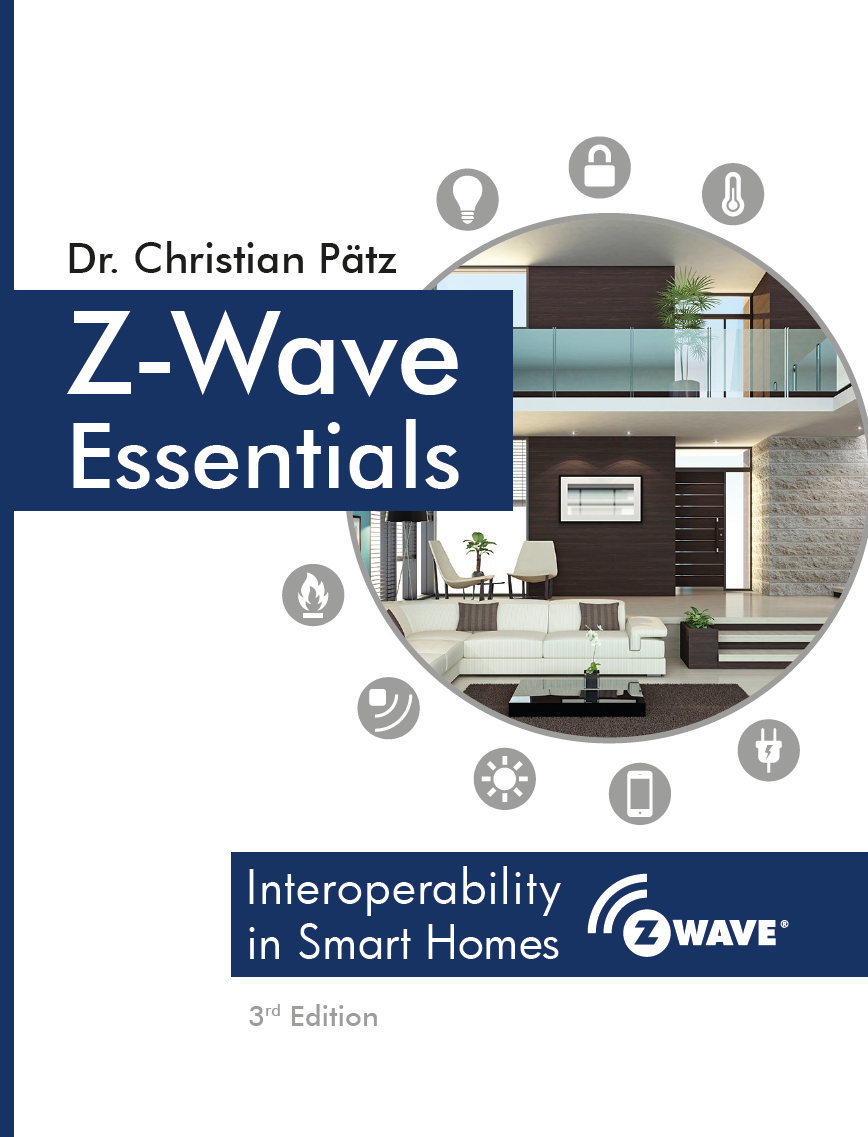
\includegraphics[width=0.4\textwidth]{pngs/cap1/zwbook.png}
\caption{Z-Wave Essentials}
\label{zwbook}
\end{center}
\end{figure}

The next chapter explains tools and processes to manage and troubleshoot \zwave networks, 
followed by explanations of how to customize the user interface to your specific needs.

The final section of the book is dedicated to developers and programmers who can, and are 
willing to, contribute to the project and/or design their own solutions based on \zway.

The need for technical understanding and knowledge increases from chapter to chapter.

Please note that this book will not provide any basic knowledge about the \zwave technology
as such. Please
refer to the book 'Z-Wave Essentials' as shown in figure \ref{zwbook} for an comprehensive
explanation of the \zwave technology. The book is available at amazon.com and many other 
book sellers. The ISBN number is 978-1545394640.


\section{History of Z-Way}

The history of \zway dates back into the year of 2008. Two developers had done their own
private \zwave controller written in Python. When they got engaged they realized that
they should combine their solutions and create a second generation \zwave controller.
The work on this merger started in May 2009 and the result - a complete \zwave controller 
written in python was certified by the Z-Wave Alliance in March 2011.

\murl{http://products.z-wavealliance.org/products/85}

To allow porting of this code to small memory platforms the whole software was rewritten
in C and Javascript was used as scripting engine. The same time the code was updated according 
the new \zwave Plus certification process and finally certified as first \zwave Plus 
compatible controller in Fall of 2014.
 
\murl{http://products.z-wavealliance.org/products/1150}
 
After many improvements the year of 2017 brought the next major change. As first software 
again \zway in Version 3.0 supports the new innovative security architecture of \zwave 
called S2.

\section{Status of the document}

The manual is based on \zway software release >= 2.3.6. Some functions marked in blue text
text require \zway v3.0.0 rc9 and up.
 
\chapter{\zway enabled Hardware}
\index{Hardware}

\zway is  a complete software solution that is ported on various hardware. In order to run 
it on a certain hardware platform, the following requirements have to be met:

\begin{enumerate}

\item There must be a binary \zway distribution available for this platform. At 
\murl{http://razberry.wave.me/z-way-server} you will find the most recent releases 
of \zway binary distributions for the various platforms supported:
	\begin{enumerate}
	\item Dune HD:  ARM Linux
	\item Alix-x86:  Intel CPU 32 Bit Linux
	\item Contactless
	\item Debian:  Intel CPU 64 Bit Linux Debian distribution
	\item Popp:  For Popp Hub, Mediatek CPU, OpenWRT
	\item Raspberry Pi: for the famous Raspberry Pi, ARM based
	\item Ubuntu: Intel CPU 64 Bit Linux Ubuntu distribution
	\item Windows: For Windows Operating System
	\end{enumerate}
Other platforms may be supported as well by one of these binary distributions.
\item \zwave transceiver connected to the platform containing a \zway license. Currently, 
the 'RaZberry Shield' always comes with an internal license enabled, while the USB Stick called UZB
needs an additional license applied. \zway may also run on platforms with embedded \zwave 
transceivers (such as Popp HUB, Dune HD set-top box), but this requires special 
arrangement with the manufacturer. Please refer to the section \ref{otherhardware} for 
more information.
\end{enumerate}

Please note that \zway will start on a certain platform without having a \zwave transceiver 
or a licensing key. However, in this case is no support for \zwave. Still, this may be a good 
starting point to test the software free of charge. Please refer to the section \ref{apps} 
for possible applications usable without having \zwave enabled.

\zwaveme currents support two basic hardware platforms with \zway licensing:

	\begin{enumerate}
	\item The RaZberry shield board for Raspberry Pi and compatible platforms
	\item The USB Stick 'UZB' for PCs, set-top boxes, NAS, etc.	
	\end{enumerate}
	
\section{RaZberry shield board for Raspberry Pi}
\index{Raspberry Pi}
\index{RaZberry}

\subsection{Compatibility}

The RaZberry shield consists of a single PCBA with a connector to the standard GPIO pin 
header connector of the Raspberry Pi minicomputer. This 25-pin header connector is 
available on all contemporary Raspberry Pi versions, such as:

\begin{itemize}
\itemsep0em
\item Version A
\item Version B
\item Version B+
\item Version 2B
\item Zero
\item Version 3
\end{itemize}

Even if your Raspberry Pi version is not on the list above, there is a very high chance 
that the shield board will work as long as your Pi has the 25-pin GPIO connector. You will 
find more information about the pinout of this 25-pin connector on various websites
\footnote{e.g. http://www.raspberry-pi-geek.de/Magazin/2015/05/Raspberry-Pi-und-Arduino-via-UART-koppeln}.

You can use other pins of the connector for other purposes as long as they do not 
physically conflict with the board.

\subsection{Pinout and options on board}

The RaZberry board use only four pins of this header connector:

\begin{itemize}
\item Gnd
\item VCC (3.3V)
\item Serial TX
\item Serial RX
\end{itemize}

Figure \ref{q1} shows how the board connects to the 25-pin header on a Raspberry Pi 2

\begin{figure}
\begin{center}
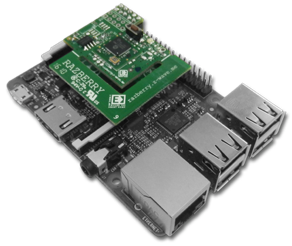
\includegraphics[width=0.4\textwidth]{pngs/cap2/q1.png}
\caption{RazBerry on top of a Raspberry Pi}
\label{q1}
\end{center}
\end{figure}

The board itself offers a few connection options as shown in Figure \ref{q2}:
\begin{enumerate}
\item Raspberry Pi Connector, used GPIO pins 1-10
\item Second open connector, identical to (1)
\item Reset button
\item Open hole for a PigTail antenna. You need to break off the PCBA antenna or unsolder 
resistor S1 to make this work.
\item Pads to solder a uFL connector for external antenna. See 
\murl{https://www.adafruit.com/products/1661} for component details. You need to break 
off the PCBA antenna to make this work.
\item Two LEDs for status information
\end{enumerate}

\begin{figure}
\begin{center}
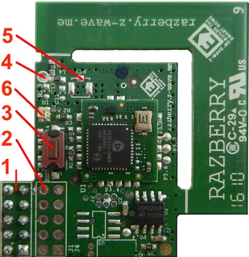
\includegraphics[width=0.4\textwidth]{pngs/cap2/q2.png}
\caption{Components on RaZberry Hardware}
\label{q2}
\end{center}
\end{figure}

The two LEDs are used to indicate the success of the boot-up self-testing and as status 
indicators during normal operation.

\subsection{Boot-Up Self-Test}

When powered up, the two LEDs light up, indicating that the self-testing has started. 
After about two seconds, they are supposed to go off indicating that that self-testing 
has been passed successfully. If they remain lit, this is a clear indication that the 
self-test failed or the device is not booting up. You will need to replace the hardware 
in such a case.

\subsection{LEDs during Operation}

During normal operation, the two LEDs remain turned off except:

\begin{itemize}
\item Green LED will light up when data is transmitted.
\item Red LED will light up when the \zwave transceiver is either in Inclusion or in 
Exclusion mode. Please note that these are special modes of the transceiver that block 
normal data communication with other nodes in the network.
\end{itemize}

\subsection{Frequencies}
\index{Frequency}

The RaZberry shield itself can be tuned into every frequency used by \zwave. However, 
to protect the transceiver and \zwave from high energy emissions on nearby frequencies 
(primarily 4G/LTE cellular radios using the 852 MHz frequency band), an external 
antenna filter is used. This limits the frequency changes to countries that share 
the same antenna filter. Currently, there are three antenna filter versions 
identified by their SKU codes.

\begin{itemize}
\item SKU: ZMEEUZB2 (865…869 MHz):
\begin{itemize}
\item Europe (EU)[default]
\item India (IN)
\item Russia (RU)
\item PR China (CN)
\item RSA (EU)
\item Middle East(EU)
\end{itemize}
\item SKU: ZMEUUZB2 (908 ... 917 MHz):
\begin{itemize}
\item All the Americas except Brazil and Peru (US) [default]
\item Israel (ISL)
\end{itemize}
\item SKU: ZMEAUZB2 (919 ... 921 MHz):
\begin{itemize}
\item Australia/New Zealand/Brazil/Peru/Malaysia (ANZ) [default]
\item Hongkong (HK)
\item Japan/Taiwan (JP)
\item Korea (KR)
\end{itemize}
\end{itemize}

There are two options to change the RaZberry operating frequency:

\begin{enumerate}
\item If you use \zweui, just choose the frontend on \menu{Network > Management} as shown in 
the figure \ref{freqchange}. For more information about this \zweui, please refer to chapter \ref{eui}.
\item There is a shell script available at
\murl{http://www.z-wave.me/fileadmin/download/changezwf.sh} 
Just execute the script with
\begin{quote}
\cmdline{changezwf.sh [COM Port] [US|EU|ANZ|…]}
\end{quote}
\end{enumerate}

\begin{figure}
\begin{center}
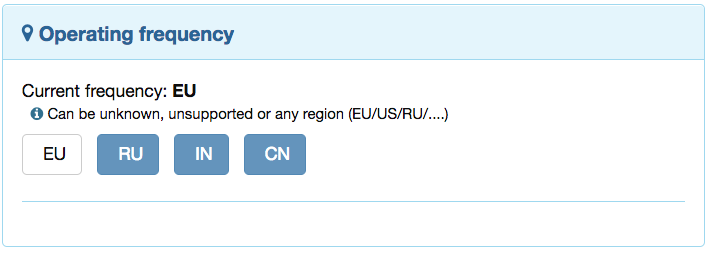
\includegraphics[width=0.6\textwidth]{pngs/cap2/freqchange.png}
\caption{Frequency Change Option in \zweui}
\label{freqchange}
\end{center}
\end{figure}

\subsection{Certifications}
\index{CE}

RaZberry is certified for use in different countries.

\subsubsection {CE / Europe}

RaZberry complies with the new Radio Equipment Directive of the European Union in general 
and the EN 300 220 version 3.1.1 in particular. The device also complies with the European ROHs and REACH regulations.

\subsubsection {FCC / North America}
\index{FCC}

The RaZberry shield was successfully tested for FCC. The FCC identifier is

\begin{quote}
\textbf{2AAYUZMEURAZ}.
\end{quote}

\subsubsection {\zwave Plus}

The RaZberry shield is a certified hardware platform and a complete solution according to 
\zwave Plus. Please refer to the certification database 
\murl{http://products.z-wavealliance.org} for more details.


\section{The USB Stick UZB}
\index{UZB}
\index{USB Stick}

The USB Stick 'UZB' allows enabling \zway on various platforms. Figure \ref{uzb} shows the device.

\begin{figure}
\begin{center}
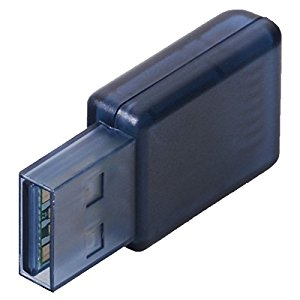
\includegraphics[width=0.3\textwidth]{pngs/cap2/uzb.jpg}
\caption{USB Stick UZB}
\label{uzb}
\end{center}
\end{figure}

It is plugged into a free standard USB port. UNIX-based operating systems will recognize 
the stick and generate a virtual serial device named
\cmdline{/dev/ttyACM0} or \cmdline{/dev/cu.usbmodem} or similar.
Windows will generate one virtual serial port \cmdline{COM XX}.

Once \zway is started, it will connect to the \zwave hardware using this virtual serial device.

The USB stick is very small (presently the smallest \zwave device in the world) and will stick quite 
close to the enclosure of the PC or NAS. This may interfere with the wireless range. 
If you experience problems with the wireless range, please use a standard USB extender 
cable to get the UZB antenna further away from the PC.

In case the UZB is not loaded with a \zway license (the stick is generally sold in two 
versions, one with a license and one without for use with 3rd party software), the 
license can be loaded once \zway is 
up and running. Please use the \zweui as described in Section \ref{eui} to apply 
the license. The license is a simple string that usually comes printed in a scratch 
card. Go to \menu{Network > Controller Info} and click on the button 
\keystroke{License Upgrade}. You will see a dialog as shown in Figure \ref{license}.


\begin{figure}
\begin{center}
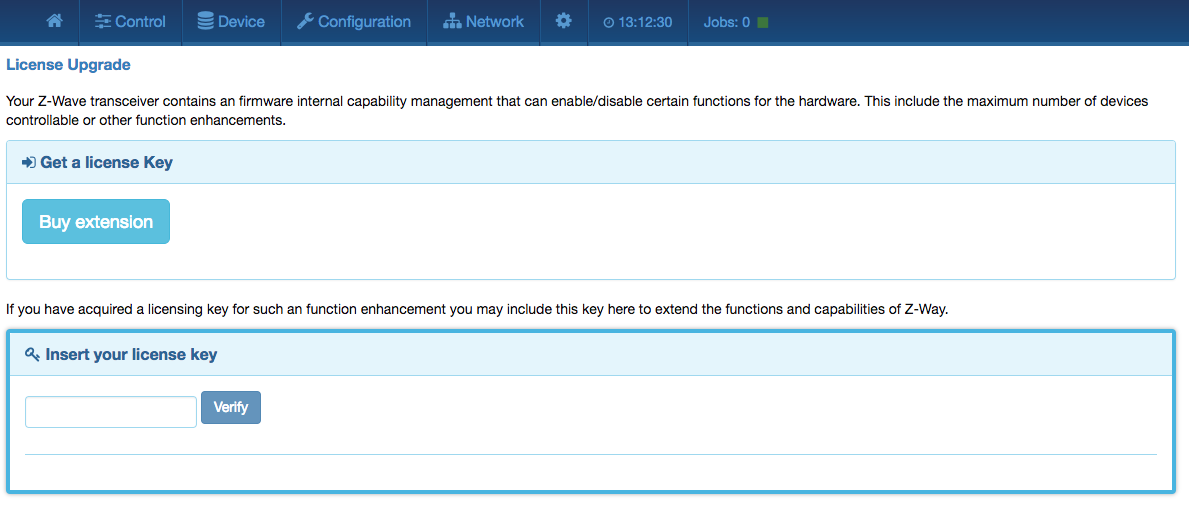
\includegraphics[width=0.9\textwidth]{pngs/cap2/licensefile.png}
\caption{UZB license upgrade}
\label{license}
\end{center}
\end{figure}

The \keystroke{Buy extension} button leads you to instructions about how to extend the 
capabilities of the UZB stick by buying extra licensing files. The input field below 
allows inserting and applying the license key manually. Please note that:

\begin{itemize}
\item You must be connected to the internet to activate the license key.
\item Every license key can only be used once (like scratch cards for prepaid phones).
\item It is possible to apply various license files to the same hardware.
\item The license is stored in the hardware. You can do a complete reinstallation of \zway on 
your platform or connect the UZB to a totally new platform without losing the license. 
However, loosing or damaging the UZB key means loosing the license!
\end{itemize}
It is possible to run multiple UZBs on one single hardware platform or even combine a 
RaZberry shield with a UZB on the same Raspberry Pi. Each piece of hardware will then 
manage its own network of \zwave devices having its own Home ID. However, \zway allows 
using devices of different \zwave networks together. This can be used to use products 
with different frequencies in one controller.

In order to enable a second \zwave transceiver (dedicated onboard, UZB or RaZberry), 
please use the standard user interface as described in Chapter \ref{shui}. 
Go to the app management section and start another instance of the app \app{\zwave Network Access}. 
Choose the new virtual serial device created by the new hardware.

Please note that the standard user interface will support devices from two networks, but 
you need to use the \zweui to manage the second network. The inclusion and exclusion 
functions of the standard user interface will always use the first \zwave network.

\subsection{Boot-Up Self-Test}

On being powered up, the blue LED will light up, indicating that the self-testing has started. 
After about two seconds, the LED goes off, indicating that that self-testing has been 
done successfully. If the LED remains lit, it means that the self-testing has failed or 
the device is not booting up. You will need to replace the hardware in such a scenario.


\subsection{Frequencies}

The \zwave transceiver itself can be tuned into every frequency used by \zwave. However, 
to protect the transceiver and \zwave from high energy emissions on nearby frequencies 
(primarily 4G/LTE cellular radios using the 852 MHz frequency band), an external antenna 
filter is used. This limits the frequency changes to countries that share the same 
antenna filter. As of now, there are three antenna filter versions identified by 
their SKU codes.

\begin{itemize}
\item SKU: ZMEEUZB2 (865…869 MHz):
\begin{itemize}
\item Europe (EU)[default]
\item India (IN)
\item Russia (RU)
\item PR China (CN)
\item RSA (EU)
\item Middle East(EU)
\end{itemize}
\item SKU: ZMEUUZB2 (908 ... 917 MHz):
\begin{itemize}
\item All the Americas except Brazil and Peru (US) [default]
\item Israel (ISL)
\end{itemize}
\item SKU: ZMEAUZB2 (919 ... 921 MHz):
\begin{itemize}
\item Australia/New Zealand/Brazil/Peru/Malaysia (ANZ) [default]
\item Hongkong (HK)
\item Japan/Taiwan (JP)
\item Korea (KR)
\end{itemize}
\end{itemize}

There are two options to change the UZB operating frequency:

\begin{enumerate}
\item If you use \zweui, just choose the frontend on \menu{Network > Management} as shown in the figure.
\ref{freqchange}. For more information about this \zweui, please refer to Chapter \ref{eui}.
\item There is a shell script available at 

\murl{http://www.z-wave.me/fileadmin/download/changezwf.sh} 
Just execute the script with

\begin{quote}
\cmdline{changezwf.sh [COM Port] [US|EU|ANZ|…]}
\end{quote}

\end{enumerate}

\subsection{Certifications}

The UZB is certified for use in different countries.

\subsubsection {CE / Europe}

The UZB complies with the new Radio Equipment Directive of the European Union in general 
and the EN 300 220 version 3.1.1 in particular. Full CE declaration can be found in
Annex \ref{annexdeclarations}.
The device also complies with the European ROHS and REACH regulations.

\subsubsection {FCC / North America}

The UZB stick shield was successfully tested for FCC. The FCC identifier is

\begin{quote}
\textbf{2AAYUZMEUUZB}.
\end{quote}

\subsubsection {\zwave Plus}

The UZB USB stick is a certified hardware platform and a complete solution according to 
\zwave Plus. Please refer to the certification database 
\murl{http://products.z-wavealliance.org} for more details.

\section {Other hardware platforms}
\label{otherhardware}

It is possible to port \zway to other hardware platforms beyond what is supported by 
binary distributions. Before contacting the \zwaveme team, you can check if your platform 
meets the requirements for \zway to run on. The general requirements are:
\begin{itemize}
\item min. 200 MHz CPU clock speed,
\item CPU architecture based on ARM, Intel or MIPS, as well as a GNU-based development tool chain,
\item min. 16 MB Flash memory and 12 MB RAM,
\item Operating system supports POSIX-compatible API.
\end{itemize}

There is a simple test to check if certain hardware on a platform is capable of running \zway.
Follow the instructions given on

\begin{quote}
\textbf{http://razberry.z-wave.me/index.php?id=28}.
\end{quote}

Only after you have double-checked that a binary distribution runs on your system or that 
the compatibility test has been passed, you may want to contact the \zwaveme team for 
further discussions about porting and licensing fees.
 % Z-Wave Device API korrigiert
\section{Executing a command from the GUI to the device and back}

\textbf{Please note that all status variables accessible on the Z-Wave Device APIs
are only are proxy of the real value in the network.}

To transport data between the real wireless device and the GUI multiple communication 
instances are involved. The complexity of this communication chain shall be 
explained in the following example:

\begin{figure} 
\begin{center}
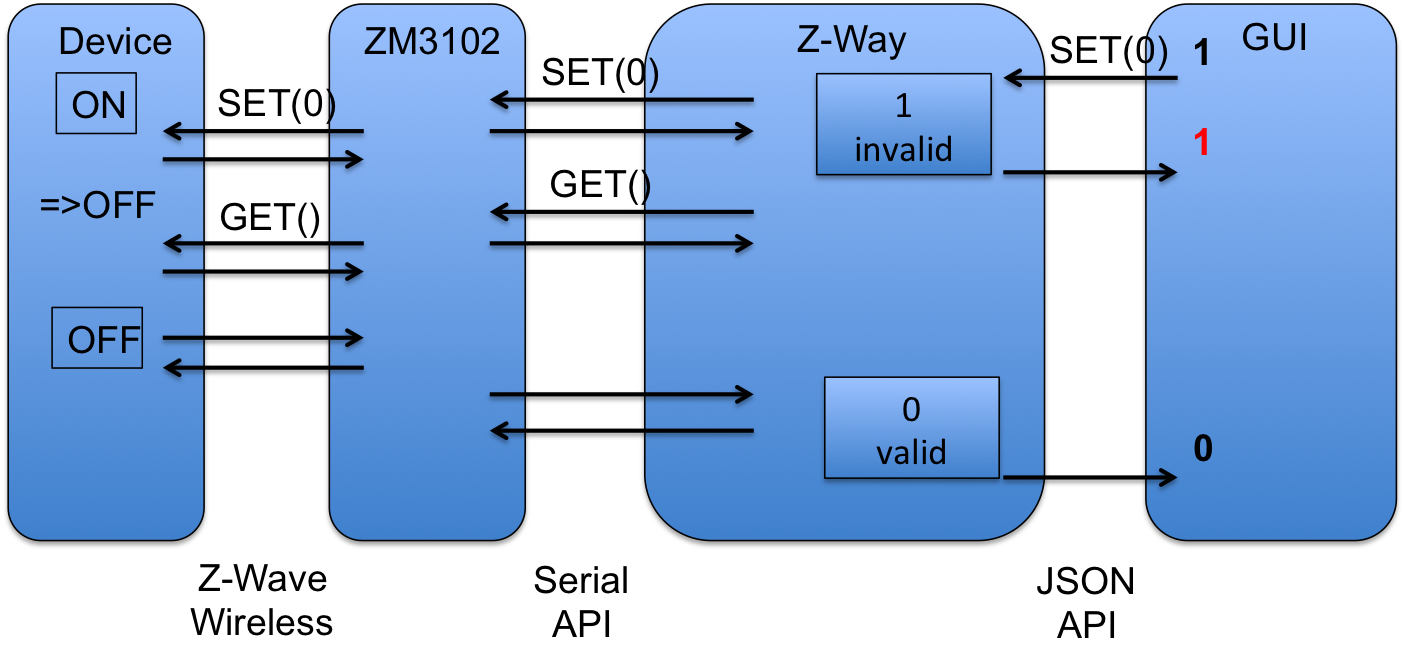
\includegraphics[scale=0.6]{pics/zway2en.png}
\caption{Z-Way Timings}
\label{zwaytimings} 
\end{center} 
\end{figure}

Assuming the GUI shows the status of a remote switch and allows to change the switching 
state of this device. When the user hits the switching button he expects to 
see the result of his action as a changing status of the device in the GUI. The first 
step is to hand over the command (SET)  from the GUI to Z-Way using the JSON interface.
Z-Way receives the command and will confirm the reception to the GUI. Z-Way recognizes 
that the execution of the switching common will likely result in a change 
of the status variable However Z-Way will not immediately change the status variable but 
invalidate the actual value. This is the correct action because at the moment
when the command was received the status is the remote device has not been changed yet 
but the status of the switch is now unknown.
If the GUI polls the value it will still see the old value but marked as invalid.
Z-Way will not hand over the switching command to the Z-Wave transceiver chip. Since it 
is possible that there are other command waiting for execution (sending) by 
the Z-Wave transceiver chip the job queue is queuing them and will handle certain 
priorities if needed. Z-Way has recognized that the command will likely change the status
of the remote device and is therefore adding another command to call the actual status 
after the switching command was issued.
The transceiver is confirming the reception of the command and this confirmation is noted 
in the job queue. This confirmation however only means that the transceiver 
has accepted the command and does neither indicate that the remote device has receives 
it nor even confirming that the remote device has executed accordingly.
The transceiver will now try to send the commend wirelessly to the remote device. A 
successful confirmation of the reception from the remote device is the only valid 
indicator that the remote device has received the command (again, not that it was executed!).
The second command (GET) is now transmitted the very same way and confirmed by the remote 
device. This device will now sent a REPORT command back to Z-Way
reporting the new status of the switching device. Now the transceiver of Z-Way has to 
confirm the reception. The transceiver will then send the new value to the Z-Way 
engine by issuing a commas via the serial interface. Z-Way receives the report and will 
update the switching state and validate the value.
From now on the GUI will receive a new state when polling.
 % Timings korrigiert
\section{The Z-Wave Device API Data model}
\label{datamodel} 
 
Z-Way holds all data of the Z-Way network  in a data holder structure. The data holder 
structure is a hierarchical tree of data elements.  

Following the object-oriented software paradigm the different commands targeting the 
network or individual devices are also embedded into the data objects as object methods.
 
Each data element is handled in a data object that contains the data element and some contextual data.

\subsection{The Data object}
 
Each Data element such as devices[nodeID].data.nodeId is an object with the following child elements:
\begin{itemize}
\item value: the value itself
\item name: the name of the data object
\item updateTime: timestamp of the last update of this particular value
\item invalidateTime: timestamp when the value was invalidated by issuing a Get command 
to a device and expecting a Report command from the device
\end{itemize}

Every time a command is issued that will have impact on a certain data holder value the 
time of the request is stored in "invalidateTime" and the "updated" flag is set to "False". 
This allows to track when a new data value was requested from the network when this new 
data value was provided by the network.

This is particularly true if Z-Way is sending a SET command. In this case the data value 
is invalidated with the "SET" commands and gets validated back when the 
result of the GET command was finally stored in the data model.

To maintain compatibility with Javascript the data object has the following methods implemented

\begin{itemize}
\item valueOf(): this allows to obmit .value in JS code, hence write as an example data.level = 255
\item updated(): alias to updateTime
\item invalidated(): alias to invalidateTime
\end{itemize}

These aliases are not enumerated if the dataholder is requested (data.level returns 
{value: 255, name: "level", 
updatedTime: 12345678, invalidatedTime: 12345678}).


\begin{figure} 
\begin{center}
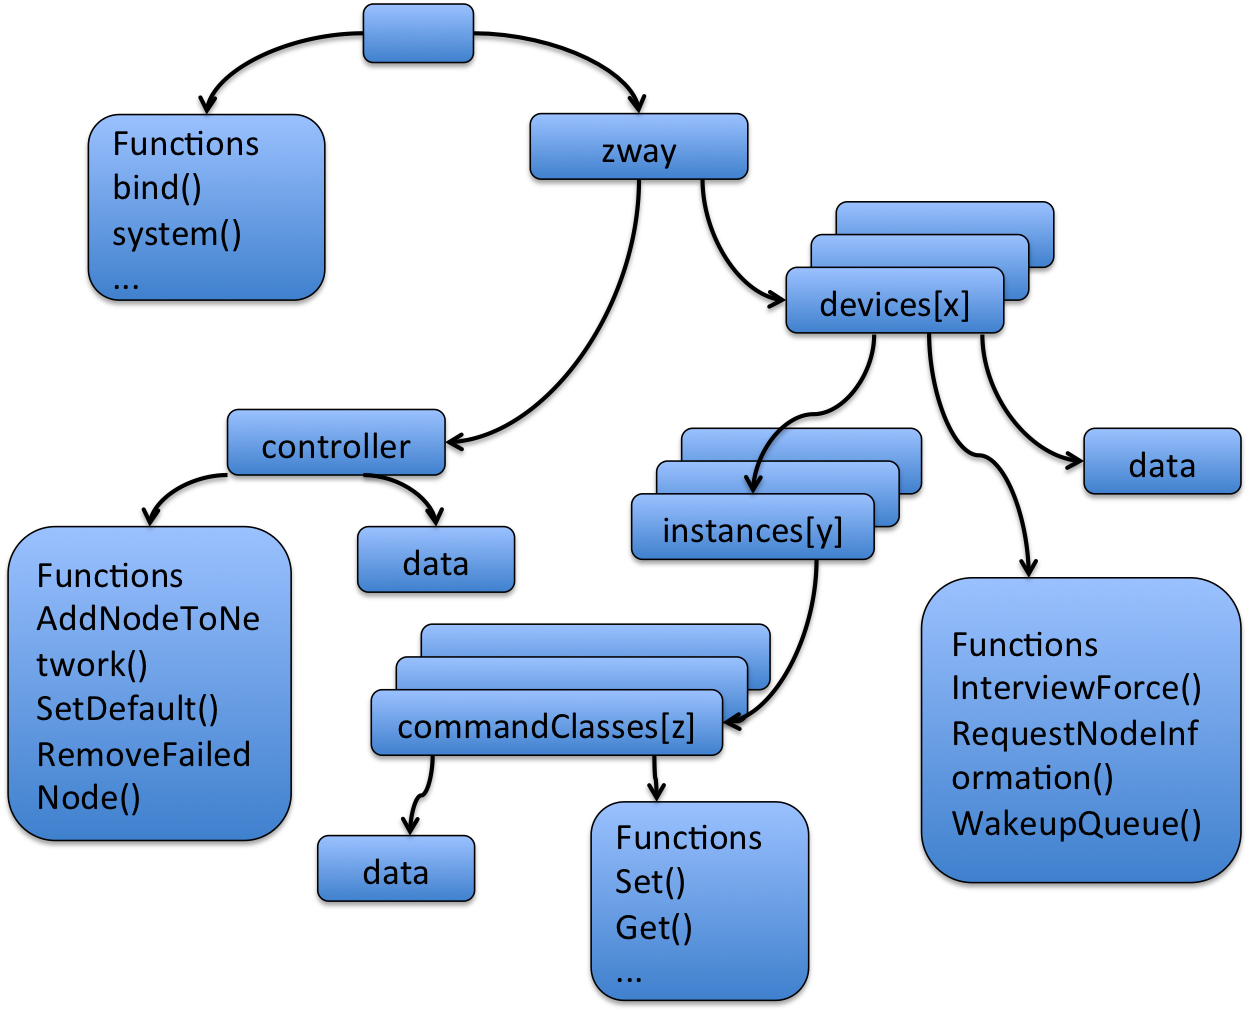
\includegraphics[scale=0.6]{pics/zwayblocks.png}
\caption{Z-Way Object Tree Structure}
\label{zwaystructure} 
\end{center} 
\end{figure} 
 
\subsection {The Data and Method Tree}
 
The root of the data tree has two important child objects:
\begin{itemize}
\item controller, this is the data object that holds all data and methods (commands,  mainly function classes) 
related to the Z-Way controller as such
\item devices array, this is the object array that holds the device specific data and methods (commands, 
mainly command classes). 
\end {itemize}

Chapter \ref{datamodel} gives a complete overview of the data and method tree.

\subsection {Device Data Visualization}

\begin{figure} 
\begin{center}
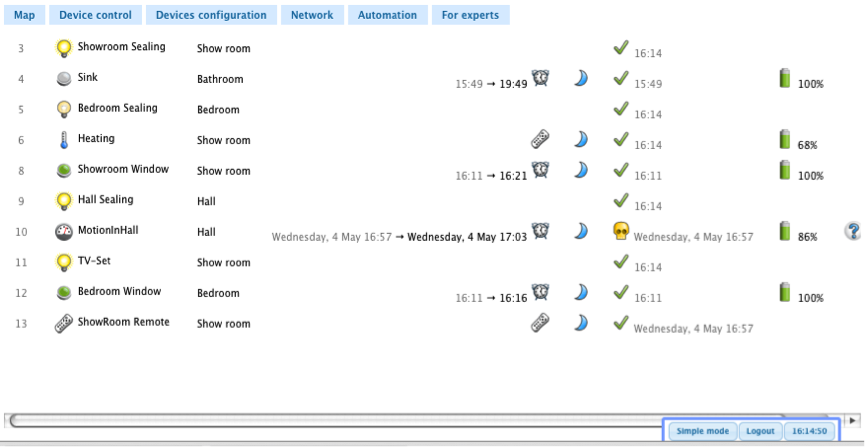
\includegraphics[scale=0.8]{pics/devicestatus.png}
\caption{Demo UI Dialog for Device Status}
\label{c4:demostatus} 
\end{center}
 \end{figure}
 
One example how to use the Data in the object tree is the device status page provided by 
the demo user interface in tab "Device Control" of the Expert UI.

 This tab gives an overview of the network status and the availability of each device. It shows the time stamp of the 
 last interaction between the controller  and the device. For battery powered devices the battery charging status, 
 the time of the last wakeup and the estimated time for the next wakeup is shown.
An info icon indicates when the interview of a device was not completed. Clicking on this device opens a window 
showing the interface status by command class. 
Please refer to the manual section “Interview” for more information about the interview process.

\begin{figure} 
\begin{center}
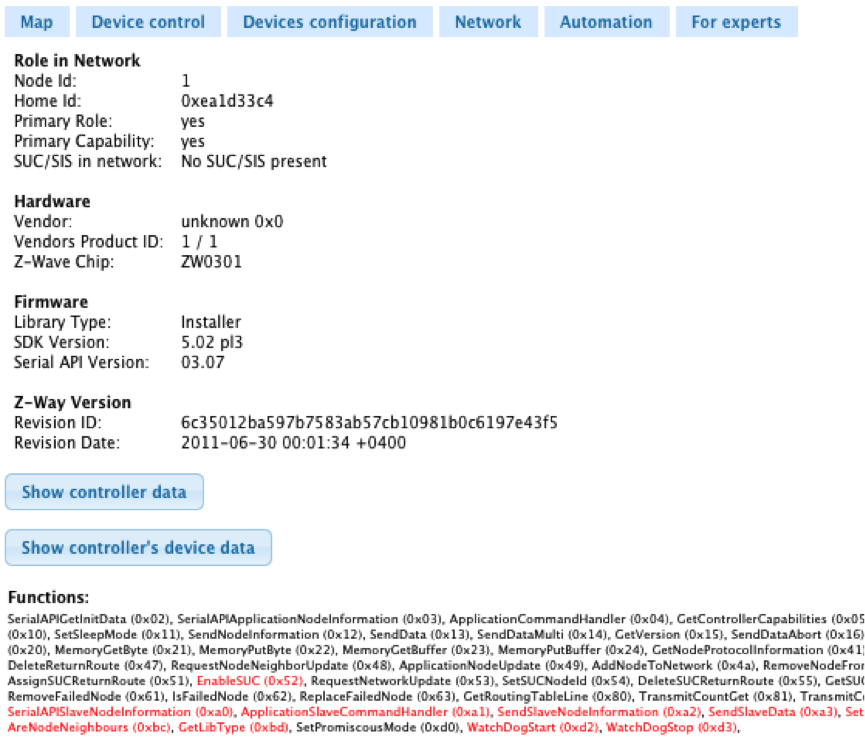
\includegraphics[scale=0.8]{pics/controllerstatus.png}
\caption{Demo UI Dialog for Controller information}
\label{c4:democontroller} 
\end{center}
 \end{figure}
  
The controller information tab shows all controller information. The buttons “Show Controller Data” shows the 
internal Z-Way data structure related to the specific controller function of the controller device. The button 
“Show controller device data” show the generic device related data of the controller device.

The information given on this page is only relevant for advanced Z-Wave developers and for debugging.

\subsection{Commands to control Z-Way itself} 
 
The last set of commands and values are not related to the Z-Wave network or the Z-Wave devices but to Z-Way itself.  
Chapter \ref{datamodel} lists all the commands and the values.

\subsection{Job Queue Handling}

The Job handling system is the core and heart of Z-Way. It is managing the different Function class and command class calls 
to the Z-Wave network and dispatches incoming messages. Every communication with the Z-Wave transceiver is scheduled 
into a job and queued that it can transmitted over the serial hardware interface. The API allows to look into the work of the job queue. 
The demo UI shows the Job queue under Tab "Network" but in expert  mode only.

\begin{figure} 
\begin{center}
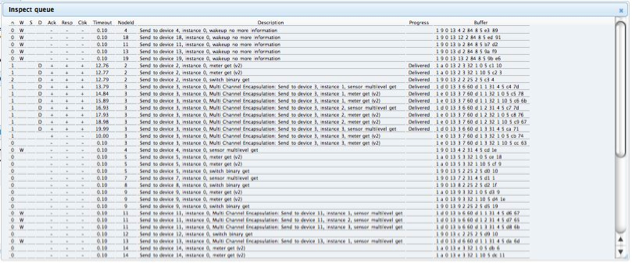
\includegraphics[scale=0.9]{pics/jobqueue.png}
\caption{Job Queue Vizualization in Demo UI}
\end{center} 
\end{figure}

The table shows the active jobs with their respective status and additional information.

\begin{table} 
\begin{tabular}{|p{0.3\textwidth}|p{0.6\textwidth}|} 
\hline
n	&This column shows the number of sending attempts for a specific job. Z-??Way tries three times to dispatch a job to the transceiver.\\ 
\hline 
W,S,D: & This shows the status of the job. If no indicator is shown the job is in active state. This means that the controller just tries to execute the job. 'W' states indicated that the controller believes that the target device of this job is in deep sleep state. Jobs in “'W' state will remain in the queue to the moment when the target devices announces its wakeup state by sending a wakeup notification to the controller. Jobs in 'S' state remain in the waiting queue to the moment the security token for this secured information exchanged was validated.
'D' marks a job as done. The job will remain in the queue for information purposes until a job garbage collection removed it from the queue.\\ 
\hline 
ACK:& shows if the Z-Wave transceiver has issued an ACK message to confirm that the message was successfully received by the transceiver. This ACK however does not confirm that the message was delivered successfully. A successful delivery of a message will result in a “D” state of this particular job.
If the ACK field is blank, then no ACK is expected. A “.” indicates that the controller expects an ACK but the ACK was not received yet. A “+” indicates that an ACK was expected and was received.\\ 
\hline
RESP	&shows if a certain command was confirmed with a valid response. Commands are either answered by a response or a callback.
If the RESP field is blank, then no Response is expected. A “.” indicates that the controller expects a Response but the Response was not received yet. A “+” indicates that a Response was expected and was received.\\ 
\hline
Cbk	&If the Cbk field is blank, then no callback is expected. A “.” indicates that the controller
expects a Callback but the Callback was not received yet. A “+” indicates that a Callback was expected and was received.\\
\hline 
Timeout	&Shows the time left until the job is de queued \\ 
\hline
Node Id	&shows the id of the target node. Communication concerning the network – like inclusion of new nodes – will have the controller node id as target node ID. For command classes command the node ID of the destination Node is shown. For commands directed to control the network layer of the protocol, the node id is zero. \\
\hline
Description	&shows a verbal description of the job \\
\hline
Progress	&shows a success or error message depending on the delivery status of the message. Since Z-Way tries three times to deliver a job up to 3 failure messages may appear.
Buffer: ... shows the hex values of the command sent within this job \\

\hline 
\end{tabular} 
\caption{Parameters of the Job Queue Vizualization} 
\label{c1:queuecommands} 
\end{table}

Table \ref{c1:queuecommands} summarizes the different values displayed on the Job Queue visualization. 
While these infos are certainly not relevant for end users of the system it is a great debug tool.  

 % Data Model korrigiert

\section{Function Class Implementation}
\label{c2:fc}

The commands used to control the controller itself and ot manage the Z-Wave network
are called 'function classes'. Most function classes used in the Sigma Designs
Serial API are used by the Z-Way lower layer function only but some of them 
are exposed to the Z-Wave Device API to allow user interactions and network management.

The Expert UI is an excellent reference for the Function Classes. All relevant functions 
can be monitored 'in action'. Hence the description of the network tab of the Expert 
UI is more or less a complete reference to the function classes needed in a UI implementation.

 
\begin{figure} 
\begin{center}
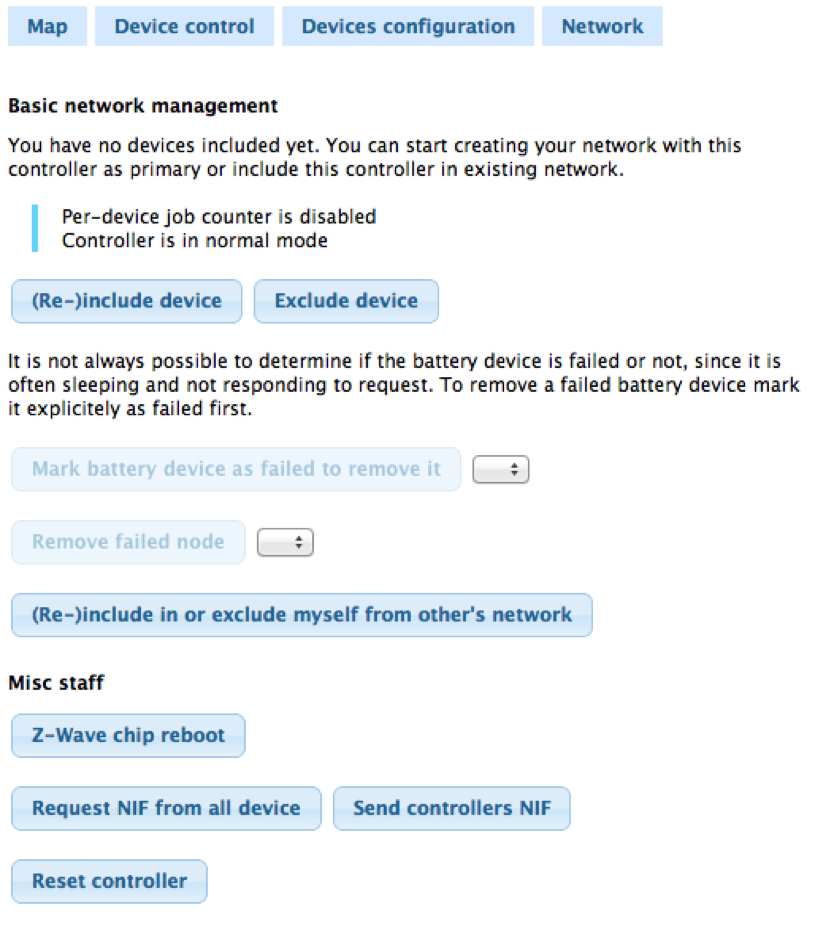
\includegraphics[scale=0.8]{pics/network1.png}
\caption{Expert UI Dialog for Networking functions}
\label{c1:network1} 
\end{center} \end{figure}

\subsection{Inclusion}

 You can include devices by pressing the 'Include Device' button. This turns the 
controller into an inclusion mode that allows including a device.  A status information 
line indicates this status. The inclusion of a device is typically confirmed with a 
triple press of a button of this particular device. However, please refer to the manual of 
this particular device for details how to include them into a Z-Wave network. The 
inclusion mode will time out after about 20 seconds or is aborted by pressing the 
'Stop Include' button.

If the network has a special controller with SIS function (Z-Way will try to activate 
such as function on default, hence this mode should always be active if the USB 
hardware used by Z-Way supports it) the inclusion of further devices can also be 
accomplished by using the include function of any portable remote control which 
is already included into the network.   A short explanation above the include button 
will inform about the ways devices can be included.

The Inclusion function is implemented using the function class 
{\bf AddNodeToNetwork(flag)} with flag=1 for starting the inclusion mode and 
flag=0 for stopping the  inclusion mode. Please refer to the chapter \ref{FunctionClasses} 
for details on how to use this function.


\subsection{Exclusion}

You can exclude devices by pressing the 'Exclude Device' button. This turns the controller 
into an exclusion mode that allows excluding a device. 
The exclusion of a device is typically confirmed with a triple press of a button of this 
particular device as well. However, please refer to the manual 
of this device for details how to exclude them into a Z-Wave network. The exclusion mode 
will time out after about 20 seconds or is aborted by pressing the 
'Stop Exclude' button.
It is possible to exclude all kind of devices regardless if they were included in the 
particular network of the excluding controller.

If a node is not longer in operation it can’t be excluded from the network since exclusion 
needs some confirmation from the device. Please use the 'Remove Failed Node' function 
in this case. 
Please make sure that only failed nodes are moved this way. Removed but still function 
nodes  - called phantom nodes – will harm the network stability.


The Exclusion function is implemented using the function class 
{\bf RemoveNodeToNetwork(flag)} with flag=1 for starting the exclusion mode and flag=0 
for stopping the 
exclusion mode. Please refer to the chapter \ref{FunctionClasses} for details on how to use this function.

\subsection{Mark Battery powered devices as failed}

This function allows marking battery-powered devices as failed. Only devices marked as 
failed can be excluded from the network without using the exclusion 
function. Typically multiple failed communications with a device result in this marking. 
Battery powered devices are recognized as sleeping in the controller 
and therefore all communication attempts with this device will be queued until a wakeup 
notification from this device is received. A faulty battery operated 
device will never send a wakeup notification and hence there is never a communication, 
which would result in a failed node status. Battery operated devices 
can therefore be manually marked as faulty.  Make sure to only mark  and subsequently 
remove  devices that are faulty or have disappeared. A device, which 
was removed with this operation but is still functioning may create malfunctions in the network.

This function is no Function class but sets the internal 'failed' variable of the device
object.

\subsection{Remove Failed Nodes}

Z-Way allows removing a node, if and only if this node was detected as failed by the 
Z-Wave transceiver. The network will recognize that communication with a device fails 
multiple times and the device can’t be reached using alternating routes either. 
The controller will then mark the device as 'failed' but will keep it in the current 
network configuration.  Any successful communication with the device will remove the 
failed mark. Only devices marked as failed can be removed using the 'Remove Failed Node' 
function.

If you want to remove a node that is in operation use the 'Exclude' Function.


This function is implemented using the function class {\bf RemoveFailedNode(node id)} 
with node id as the node id of the device to be removed. Please refer to the chapter 
\ref{FunctionClasses} for details on how to use this function. It is also possible to 
replace a failed node by a new node using the function class {\bf RemoveFailedNode(node id)}. 
Please refer to the  chapter \ref{FunctionClasses} for details too.

The function {\bf IsFailedNode(node id)} can be used to detect if a certain node is 
failed. The Z-Wave transceiver will try to contact the device wirelessly and will then 
update the failed-status inside the transceiver and also the 'is failed' flag of the 
device object in Z-Way.

\subsection{Include into different network}

Z-Way can join a Z-Wave network as secondary controller. It will change its own Home ID to the Home ID of the new network and it will learn all network information 
from the including controller of the new network. To join a different network, the primary controller of this new network need to be in the inclusion mode.

Z-Way needs to be turned into the so called learn mode using the button 'Start Include in 
others network'. The button “Stop Include in others network” can be used to turn off 
the Learn mode, which will time out otherwise or will stop if the learning was successful.

Please be aware that \textbf{all existing relationships to existing nodes will get lost} 
when the Z-Way controller joins a different network. Hence it is recommended to join a 
different network only after a reset with no other nodes already included. 

The 'Learn' function is implemented using the function class {\bf SetLearnMode(flag)} 
with flag=1 for starting the learn mode and flag =0 for stopping the learn mode. Please 
refer to the chapter \ref{FunctionClasses} for details on how to use this function.


\subsection{Z-Wave chip reboot}

This function will perform a soft restart of the firmware of the Z-Wave controller chip 
without deleting any network information or setting. It may be necessary to recover the 
chip from a freezing state. A typical situation of a required chip reboot is if the 
Z-Wave chip fails to come back from the inclusion or exclusion state.

The reboot function is implemented using the function class {\bf SerialAPISoftReset()}.  
Please refer to the chapter \ref{FunctionClasses} for details on how to use this function.


\subsection{Request NIF from all devices}

This function will call the Node Information Frame from all devices in the network. 
This may be needed in case of a hardware change or when all devices 
where included with a portable USB stick such as e.g. Aeon Labs Z-Stick.  Mains powered 
devices will return their NIF immediately, battery 
operated devices will respond after the next wakeup.


This function controls a Z-Way controller function that will send out a function 
class {\bf RequestNodeInformation(node)} to all nodes in the network. 
The function can also be called for one single node only. Please refer to the 
chapter \ref{FunctionClasses} for details on how to use this function.

\subsection{Send controllers NIF}

In certain network configurations it may be required to send out the Node Information 
Frame of the Z-Way controller. This is particularly useful for some some remote 
controls scene activation function. The manual of the remote control will refer to this 
requirement and give further information when and how to use this function.

This function is implemented with the function class {\bf SerialAPIApplicationNodeInfo} 
with plenty of parameters. These parameters are partly set by Z-Way but particularly the 
Command classes supported (parameter 'NIF') can be changed by editing the file defaults.xml. 
Please refer to the chapter \ref{FunctionClasses} for details on how to use this function 
the chapter about the translation files on how to change defaults.xml

\subsection{Reset Controller}

The network configuration (assigned node Ids and the routing table and some other network 
management specific parameters) is stored in the Z-Wave 
transceiver chip and will therefore even survive a complete reinstallation of the Z-Way software.

The function 'Reset Controller' erases all values stored in the Z-Wave chip and sent the 
chip back to factory defaults. This means that \textbf{all network information will be lost 
without recovery option}.

This function is implemented with the function class {\bf SetDefault()}. Please refer 
to the chapter \ref{FunctionClasses} for details on how to use this function.

\subsection{Change Controller }

\begin{figure} 
\begin{center}
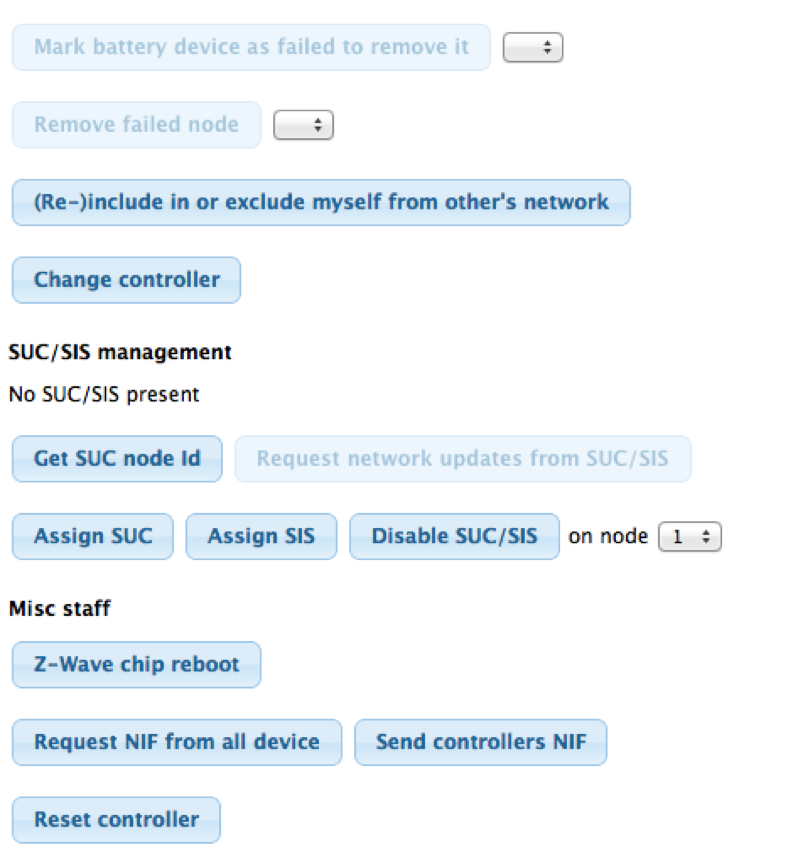
\includegraphics[scale=0.8]{pics/network2.png}
\caption{Demo UI Dialog for Networking functions - experts functions}
\label{c1:network2} 
\end{center} \end{figure}


The controller change function allows to handover the primary function to a different 
controller in the network. The function works like a normal inclusion 
function but will hand over the primary privilege to the new controller after inclusion. 
Z-Way will become a secondary controller of the network. This function may be needed 
during installation of larger networks based on remote controls only where Z-Way is 
solely used to do a convenient network 
setup and the primary function is finally handed over to one of the remote controls.

This function is implemented with the function class {\bf ControllerChange()}. Please 
refer to the chapter \ref{FunctionClasses} for details on how to use this function.

\subsection {SUC/SIS Management}

This interface allows controlling the SUC/SIS function for the Z-Wave network. All 
these functions are almost obsolete and only needed for certain enhanced configurations 
of the Z-Wave network. Unless you really know what you do - don't use these functions!

The following Function Classes are mapped to the demo user interface  functions 
for SUC/SIS manipulation:
\begin{itemize}
\item GetSUCNodeId - get the SUC Node ID from the network
\item EnableSUC - enables the SUC function in Z-Way, this is done by default if the transceiver firmware used supports SUC
\item SetSUCNodeId - assign SUC function to a node in the network that is capable of running there SUC function.
\item SendSUCNodeId - inform a different node about the node ID of a SUC in the system
\end{itemize}


 
\subsection{Routing Table}


\begin{figure} 
\begin{center}
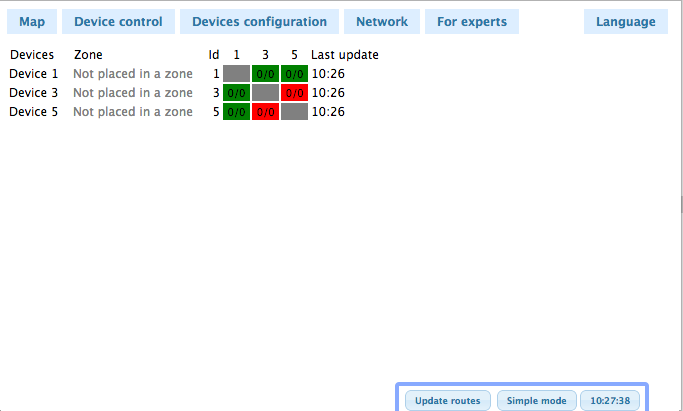
\includegraphics[scale=0.5]{pics/routingtable.png}
\caption{Demo UI dialog for Routing Table}
\label{c2:demorouting} 
\end{center} \end{figure}

The routing table of the Z-Wave network is shown in the tab network as well. It indicates how two devices of the Z-Wave network can communicate with each other. 
If two devices are in direct range (they can communicate without the help of any other node) the cross point of the two devices in the table is marked as dark green. 
The color light green indicates that the two nodes are not in direct range but have more than one alternating routes with one node between. This is still considered 
as a stable connection.
The yellow color indicates that there are less than two “one-hop” routes available between the two nodes. However there may be more routes but with more nodes
 between and therefore considered as less stable.

A red indicator shows that there are no good short connections between the two nodes. This does not mean that they are unable to communicate with each other 
 but any route with more than 2 routers between Z-Way is considering as not reliable, even taking into account that Z-Wave supports routes with up to four devices 
 between. Grey cells indicate the connection to the own Node ID. 

The general rule of thumb is: 'The greener the better'.
 
The table lists all nodes on the y-axis and the neighborhood information on the x-axis. On the right hand side of the table a timestamp shows when the neighborhood
 information for a given node was reported.   

In theory the table should be totally symmetric, however different times of the neighborhood detection may result in different neighborhood information of the 
two devices involved.
 
The neighbor information of the controller works with an exception. The Z-Wave implementation used in current Z-Wave transceiver does not allow requesting an 
update of the neighbor list for the controller itself. The neighborhood information displayed for the controller is therefore simply wrong.

Battery powered devices will report their neighbors when woken up and report their mains powered neighbor correctly. However mains powered devices will report 
battery-powered devices as neighbors only when routes are updated twice. This is less critical because battery powered devices can’t be used as routers and are 
therefore not relevant for calculating route between two nodes anyway. 
 
The context menu command 'Network Reorganization' allows re-detecting all neighborhood information (battery powered devices will report after their next wakeup!) 
Please refer to the manual section 'Network Stability' for further information about the use of this function.

The routing table is stored in the Z-Wave transceiver and can be read using the function class {\bf  GetRoutingTableLine(node id)} for a given node ID. The function 
{\bf RequestNodeNeighbourUpdate(nodeid)} will cause a certain node Id to redirect its
 wireless neighbors. It makes sense to call the GetRoutingTable function right 
after successful callback of the RequestNodeNeighbourUpdate function. 

  % Function Classes
\section{JSON-API}
\label{jsapi}
JSON API allows to execute commands on server side using HTTP POST requests 
(currently GET requests are also allowed, but this might be deprecated in future). 
The command to execute is taken from the URL.

All functions are executed in form 

\paragraph{http://YOURIP:8083/$<$URL$>$}


\subsection{/ZWaveAPI/Run/$<$command$>$}

This executes zway.$<$command$>$ in JavaScript engine of the server. As an example to 
switch ON a device no 2 using the command class BASIC (The ID of the command class BASIC is 0x20, for more
information about the IDs of certain command classes please refer to the Annex) its 
possible to write:

\begin{quote}/ZWaveAPI/Run/devices[2].instances[0].commandClasses[0x20].Set(255)\end{quote}

or

\begin{quote}/ZWaveAPI/Run/devices[2].instances[0].Basic.Set(255)\end{quote}



The Z-Way Expert GUI has a JavaScript command runCmd($<$command$>$) to simplify such 
operations. This function  is accessable in the Javascript console of your web browser 
(in Chrome you find the JavaScript  console unter View-$>$Debug-$>$JS Console). Using 
this feature the command in JS console would look like

\begin{quote}runCmd('devices[2].instances[0].Basic.Set(255)')\end{quote}


The usual way to access a command class is using the format \\'devices[nodeId].instances[instanceId].
commandClasses[commandclassId]'.
There are ways to simplify the syntax:

\begin{itemize}
\item 'devices[nodeId].instances[instanceId].Basic' is equivalent to \\
'devices[nodeId].instances[instanceId].commandClasses[0x20]'
\item the instances[0] can be obmitted: 'devices[nodeId].instances[instanceId].Basic' 
then turns into 'devices[nodeId].Basic'
\end{itemize} 

Each Instance object has a device property that refers to the parent device it belongs to. 
Each Command Class Object has a device and an instance property that refers to the instance 
and the device this command class belongs to.
 

Data holder object have properties value, updateTime, invalidateTime, name, but for 
compatibility with JS and previous versions we have valueOf() method (allows to 
omit .value in JS code, hence write "data.level == 255"), updated (alias to updateTime), 
invalidated (alias toinvalidateTime). These aliases are not enumerated if the dataholder 
is requested (data.level returns {value: 255, name: "level", updatedTime: 12345678, 
invalidatedTime: 12345678}).

\subsection{/ZWaveAPI/InspectQueue}

This function is used to visualize the Z-Way job queue. This is for debugging only but 
very useful to understand the current state of Z-Way engine.

\subsection{/ZWaveAPI/Data/$<$timestamp$>$}
Returns an associative array of changes in Z-Way data tree since $<$timestamp$>$. The 
array consists of ($<$path$>$: $<$JSON object$>$) object pairs. The client is supposed 
to assign the new $<$JSON object$>$ to the subtree with the $<$path$>$ discarding previous 
content of that subtree. Zero (0) can be used instead of $<$timestamp$>$ to obtain the 
full Z-Way data tree.

The tree have same structure as the backend tree (Figure \ref{zwaystructure}) with 
one additional root element "updateTime" which contains the time of latest update. 
This "updateTime" value should be used in the next request for changes. 
All timestamps (including updateTime) corresponds to server local time.

Each node in the tree contains the following elements:
\begin{itemize}
\item value — the value itself
\item updateTime — timestamp of the last update of this particular value
\item invalidateTime — timestamp when the value was invalidated by issuing a Get 
command to a device and expecting a Report command from the device
\end{itemize}

The object looks like:
\begin{lstlisting}[caption=JSON Data Structure]{Name}
{
"[path from the root]": [updated subtree],
"[path from the root]": [updated subtree],
...
updateTime: [current timestamp]
}
\end{lstlisting}

Examples for Commands to update the data tree look like:

\begin{quote}Get all data: /ZWaveAPI/Data/0\end{quote}

\begin{quote} Get updates since 134500000 (Unix timestamp): /ZWaveAPI/Data/134500000\end{quote}

Please note that during data updates some values are updated by big subtrees. For example, 
in Meter Command Class value of a scale is always updated as a scale subtree by 
[scale].val object (containing scale and type descriptions).


\subsection{Handling of updates coming from Z-Way}

A good design of a UI is linking UI objects (label, textbox, slider, ...) to a certain 
path in the tree object. Any update of a subtree linked to UI will then update the UI too. 
This is called bindings.

For web applications Z-Way Web UI contains a library called jQuery.triggerPath 
(extention of jQuery written by Z-Wave.Me), that allows to make such links between 
objects in the tree and HTML DOM objects. Use

\begin{quote}var tree;\end{quote}
\begin{quote}jQuery.triggerPath.init(tree);\end{quote}

during web application initialization to attach the library to a tree object. Then run

\begin{quote}jQuery([objects selector]).bindPath([path with regexp], [updater function], 
[additional arguments]);\end{quote}

to make binding between path changes and updater function. The updater function would be 
called upon changes in the desired object with this pointing to the DOM object itself, 
first argument pointing to the updated object in the tree, second argument is the exact 
path of this object (fulfilling the regexp) and all other arguments 
copies additional arguments. RegExp allows only few control characters: * 
is a wildcard, (1|2|3) - is 1 or 
2 or 3.  

\textbf{Please not that the use of the triggerpath extension is one option to handle the incoming
data. You can also extract all the interesting values right when the data is received and 
bind update functions to them.} % JSON
\section{Command Class Implementation} 
 
Z-Wave device functions are controlled by command classes. A command class can be have one or  multiple commands
allowing the use of a certain function of the device. Command classes are organized by functions, e.g. the command class "Switch Binary" allows to switch 
a binary switch. Hence the number of supported command classes defines the functionality and the value of 
a device.

Z-Wave defines quite a few command classes but a lot of them are not implemented in any device. Hence, Z-Way will not implement them 
either. Command Classes consist of two types of commands:
\begin{itemize}
\item commands for users, most of them are either "GET" commands asking for a value or status from a remote device, or they are "SET" commands setting
 a certain value and therefore causing a certain action.
\item commands for configuration
 \end{itemize}

The commands for configuration are used by Z-Way to build the data model used and to manage the device itself but they are not made public for users. 
The command classes available for users are listed in chapter \ref {ccs}.

Commands to Z-Wave devices take time to be executed. In case the device is awake (mains powered or FLIRS) the delay may be well below one second but for 
battery powered  devices the controller has to wait for the next scheduled wakeup in order to send the command. 

In case the command is calling a value update from e.g. a sensor the successful execution of the command only means that the request was accepted by the
wireless device. In order to really update a value the device itself needs to send a wireless command back to the controller that needs to be accepted by the 
controller.    

Each data element that is available in a remote wireless device (e.g. a switch) is also stored in  Z-Way. First of all there is the assumption that the data value of the remote device
and the corresponding data value in Z-Way are identical.

 Most commands of command classes are eighter a "GET" asking for an update of an value or they are a "SET" - setting a new value. Setting a new 
 value may also cause an action on the remote side. As an example switching a binary switch means in Z-Wave command classes changing the switching  
 state value wirelessly.

Z-Way will never "just" update the local corresponding value of the real remote value but always ask the remote device after a successful "SET"  command for 
an update of the remote value using a "GET" command.  This means that the local  - displayable - value of a certain remote device will only update after some delay.

The process can be examined using the "Device Control" dialog in the Expert User Interface.

 
\subsection{Switch Overview}



\begin{figure} 
\begin{center}
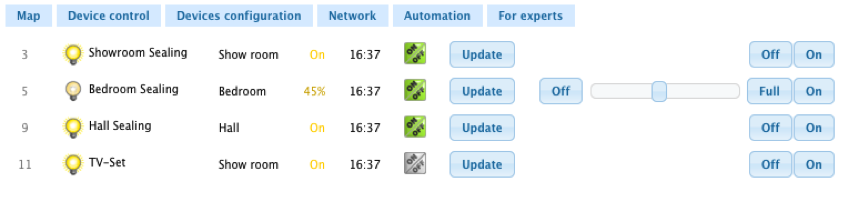
\includegraphics[scale=0.8]{pics/switches.png}
\caption{Demo UI Dialog for Switches}
\label{c3:demosen} 
\end{center}
 \end{figure}
This page gives a table style overview of all actuators of the Z-Wave network. Actuators are devices with some kind of switching function such as 

\begin{itemize}
\item Digital (on/off) switches, 
\item Light Dimmer, 
\item Motor Controls for Venetian blinds, window bind,
\item Motor Control to open/close doors and windows.
\end{itemize}

Beside the name of the device, the location and the type of device the actual status and the timestamp of this status are shown.

Of course it is possible to switch the devices and to update the status of the device.

A little icon indicates how the device will react to a “switch all devices” command  (will switch, will 
not switch, will react to off command only or to on command only).

The commands to control the different actors apply the  command classes "Switch Multilevel" and "Switch 
Binary". Please refer to Chapter \ref{ccs} for details how to use these command classes.


\subsection{Sensor Overview}


\begin{figure} 
\begin{center}
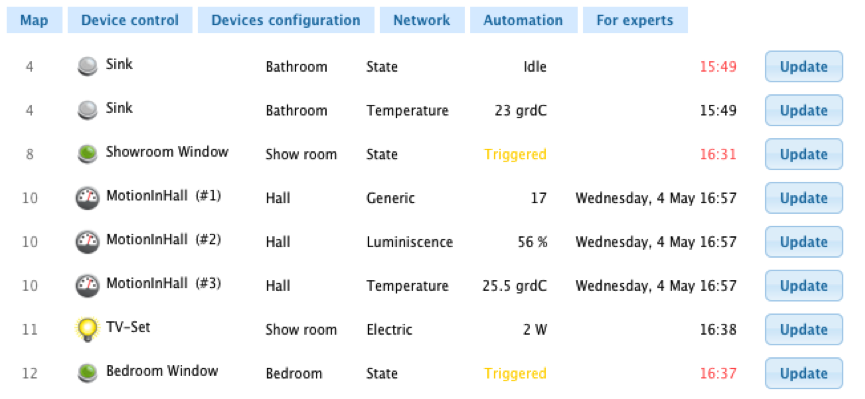
\includegraphics[scale=0.5]{pics/sensors.png}
\caption{Demo UI Dialog for Sensors}
\label{c3:demosensor} 
\end{center}
 \end{figure}

 This page gives a table style overview of all sensors of the Z-Wave network.  
Sensors are devices able to report measured values. Sensors can report binary or analog values.  Beside the name of the device, the location and the type of sensor the actual sensor value and the timestamp of this value are shown. It is possible to ask for an update of the sensor value.

 
 
The update command of the sensor interface and  the values shown are using the command classes "Sensor Multilevel" and "SensorBinary". Please refer to Chapter \ref{ccs} for details how to use these command classes.
 
\subsection{Meter Overview}

This page gives a table style overview of all meters of the Z-Wave network.  
Meters are devices able to report accumulated values.  Beside the name of the device, the location and the type of meter the actual meter value and the timestamp of this value are shown. It is possible to ask for an update of the meter value.
 
The update command of the meter interface and the values shown are using the command class "Meter". Please refer to Chapter \ref{ccs} for details how to use the meter command class.

\subsection{Thermostat Overview}

This page gives a table style overview of all thermostats of the Z-Wave network.  
Depending on the thermostat capabilities reported, the dialog will allow to change the thermostat mode and/or change the setpoint temperature 
for the thermostat mode selected.
 
Please refer to Chapter \ref{ccs} for details how to use the thermostat setpoint and thermostat mode command classes.

\subsection{Door Lock Overview}

This page gives a table style overview of all door locks of the Z-Wave network.  
Depending on the door lock reported, the dialog will allow to open/close the door
and differentiate on door handles.
 
Please refer to Chapter \ref{ccs} for details how to use the door lock, user code
and door lock logging command classes.


 
 
\subsection{Device Configuration} 
 
Beside the command class to directly control devices and update device values there are more 
commands that are used to built the data model of the device and to get configuration values. 

The device also allow certain configurations itself. The demo UI shows the use of these command classes in the Tab "Device Configuration". The device configuration fulfills three basic tasks:

\begin{itemize}
\item The interview process after inclusion of the device
\item The configuration of the device according to user requirements and needs.
\item Setting Cause/effect relationships. This means that certain devices can directly control other devices.

\end{itemize}


\subsection{Interview Process}
After the inclusion of a new device Z-Way will interview this very device. The interview is a series of commands Z-Way is sending 
to the device in order to learn the capabilities and functions of this device.


Depending on the capabilities announced in the Node Information Frame that was received during the inclusion, Z-Way will ask further 
questions to get more detailed information. The interview process may take some seconds since more questions may be required to ask depending in certain answers given.
Since all functions of a device are grouped in so called Command Classes each command class announced in the Node Information frame will typically cause its part of the interview.
The interview will be executed in three different steps:

\begin{enumerate}
\item In case there is a Version Command Class ask for the Version of the device and the versions of all Command Classes announced in the Node Information frame. Otherwise Version 1 is assumed.
\item In case there is a Multi Channel Command class announced, ask for the number of the capabilities of the different channels and repeat Step 3 for each channel.
\item Ask for all capabilities of all command classes.
\item Do some auto configurations if needed.
\end{enumerate}

The „Device Status“ tab will indicate if the interview was successfully completed.  The blue information icon shows if the interview was not complete. Clicking on this icon opens a dialog with all command classes and the status of their respective interviews.  
A complete interview is important in order to have access to all functions of the device included. Incomplete interviews may also be a reason for malfunctions of the network.
There are several reasons why an interview may not be completed.
\begin{enumerate}
\item A battery-operated device may be gone into sleep mode too early. In this case it is possible to wake up the device manually to complete the interview. Sometimes manual wakeup is needed several times.
\item The device does not fully comply with the Z-Wave protocol. This is particularly possible for devices that were brought to market before 2008. 
The current more sophisticated certification process makes sure that devices are 100\% compatible to the Z-Wave product when they hit the market. 
Please check online ressources on wikis and forums for further details and possible ways to fix these kinds of problems.
\item The device does not have a reliable communication route to the controller. Interview communication typically use longer packets than normal polling communication. This makes the interview communication more vulnerable against weak and instable communication links. Its possible that the controller is able to include a device and even receive confirmation of a polling request but still not being able to complete the interview. However this is a rare case.
\item The device may be simply broken.

\end{enumerate}

Most of the command exchange during interview is using commands dedicated for the interview process. They are not exposed on the API.

\subsection{Device Configuration} 


Each Z-Wave device is designed to work out of the box after inclusion without further configuration. 
However, it may be suitable and in certain contexts even required to do a device specific configurations.

The device configuration page allows to further configure the device and to access certain additional 
information about the device. The tab is grouped into several sections. The sections can be toggled 
from invisible to visible and back by clicking on the headlines:
\begin{itemize}
\item Select Z-Wave Device Description Record
\item Device Description
\item Configurations
\item Actions with configurations
\item Advanced Actions
\end{itemize}

\paragraph{Select Z-Wave Device Description Record}

After a successful inclusion Z-Way will interview the device to gather further information.  

Certain information such as names of association groups, the brand name of the device and the parameters of further configuration values can not be detected during interview. 
Z-Way uses a device database with product description files to obtain this information. In order to identify the right device description record, certain parameters of the interview are used. 
If these parameters match exactly one device description record, this very record is loaded and its content is shown on the device configuration page automatically.

If the information from the device is sufficient to select one specific record from the database this section of the tab is hidden. 
If it is not possible to identify the correct device description record the user can manually choose the correct record. It is also possible to manually 
change the selection of the device description by unhiding this section and clicking on the “Select Device Description Record” button.

\paragraph{Device Description}

The upper part of the dialog shows some descriptive values of the device.  The Z-Wave device type is the only value generated solely from the interview data. All other data are taken from the device description record.
\begin{itemize}
\item Zone: ... the zone/room the device is assigned to. Will be manually defined in Zone-tab.
\item Brand: … the product code or brand name of the device. This will be taken from the device description record.
\item Device Type: ... the type of Z-Wave device as reported by the device during inclusion.
\item Description: … a verbal description of the function. This will be taken from the device description record.
\item Interview Stage: …shows the progress of the interview process. This information is generated by Z-Way.
\item Inclusion Note: … how to (re-) include the device. This will be taken from the device description record.
\item Wakeup Note: … this will be taken from the device description record.
\item Documents: … If the device description record offers links to manuals or other online documents there are shown here. This will be taken from the device description record.
\item Device State:  Status of the device plus number of packets queued for this device
 \end{itemize}

\begin{figure} 
\begin{center}
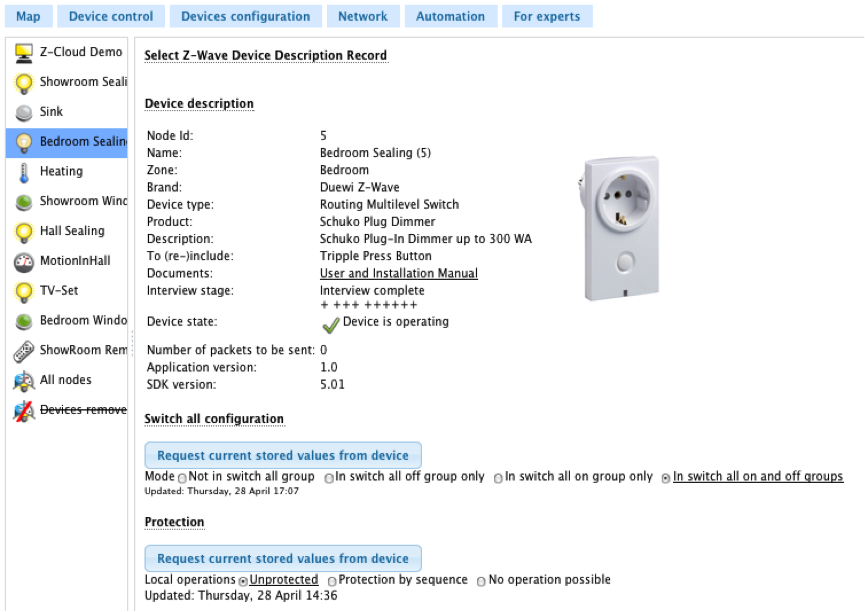
\includegraphics[scale=0.7]{pics/dconfig.png}
\caption{Demo UI Dialog for Sensors}
\label{c1:demosensors} 
\end{center}
 \end{figure}


There are a couple of reasons why no device description record was found:
\begin{enumerate}
\item There is no record for the device available. Since there are always new devices on the market Z-Way needs to catch up and update its device database. If your device is not found, updating to the most recent version of Z-Way may help.
\item The interview was not finished to the point where enough parameters were detected to identify the correct device description record. You may manually choose the correct device description record using the button “Select Device Description Record”. A dialog box will be opened for manual selection of the product (if available). The manual selection of a device description record is only needed if no record was found on default.  
\item The interview of the device was completed but the device does not offer enough information to identify the correct device. You may manually choose the correct device description record using the button “Select Device Description Record”. A dialog box will be opened for manual selection of the product (if available). The manual selection of a device description record is only needed if no record was found on default.
\item There is more than one device description record matching the information gathered during interview.  This is particularly possible if a vendor sells devices with different firmware and functions without properly updating the firmware version information. You may manually choose the correct device description record using the button “Select Device Description Record”. A dialog box will be opened for manual selection of the product (if available). The manual selection of a device description record is only needed if no record was found on default.
\end{enumerate}

\paragraph{Device Configuration}

This section will, if device description record is loaded,  show device specific configuration values including their possible parameters and a short description of the configuration value. You may change these values according to your needs.

\paragraph{Actions with configurations}

The most important action in regard to the configuration is to apply the configuration to the device. This is only done when the button “Apply configuration for this device” is hit. This button is therefore even shown, when the rest of the tab part is hidden.
\begin{itemize}
\item Mains Powered Devices: The settings will become effective immediately after hitting the button.
\item Battery Powered Devices: The settings will become effective after the next wakeup of the device, as shown in the Device Status tab.
\item Battery Powered Controllers (remote controls or wall controllers): The settings will only become effective if the devices are woken up manually. Refer to the controller manual for more information on how to wake up the device. Appendix B may also give further advice.
\end{itemize}

If there are many similar devices in a network, it is desirable to just apply one working configuration to all these devices. This can be done using the function 'Copy from other Device'.

The set of defined configuration values is stored for every device. Therefore its possible to pick a different device and reuse its configuration values for the device to be configured.  
The „Save“ function of the bottom context menu allows saving the configuration for further use and reuse.

\paragraph{Actions with configurations} 

This function requests the selected device to send its Node Information frame (NIF) to the controller. It can be used instead of triple pressing a button on the device itself that would also instruct the device 
to send it NIF. The NIF is needed to know device capabilities.

\paragraph{Delete Configuration of this device – in section “Actions with configuration”}

This function deletes the stored configuration for this device. This function is for debugging purposes only.

\paragraph{Force Interview – in section “Advanced”}

This functions forces to redo the whole interview. All previous interview data will be deleted. This function is for debugging purposes only.

\paragraph{Show Interview Results – in section “Advanced”}

This function shows the result of the interview. This function is for debugging purposes only. For information about reasons for incomplete interview please refer to the manual section “Device Status”.

The bottom context menu function  „Reset Configuration“ deletes all configurations stored in Z-Way, but does not affect devices!



The configuration dialog documents the use of the command classes "Association", "Protection", "Configuration" and "Switch All".
  
\subsection{Associations}


If there was no previous device of the same type installed, the interface will show the values as read from the device. If there was already a device of the same kind installed, there may exist a stored default configuration for this particular device. Then the setup in the device may differ from the default configuration stored in Z-Way.
\begin{itemize}
\item Gray Icon: This Node ID is stored in the device but its not stored in the default configuration of the Z-Way. You can double click this device to store this setting in the Z-Way default configuration of this device type.
\item Red Icon: This Node ID is stored locally but not in the association group of the device yet. Apply the settings to transmit the setting into the device.  In case of a battery operated device you need to wakeup the device in order to store the configuration.
\item Black Icon: This Node ID is stored both in the device and in the local configuration of Z-Way.
\end{itemize}
Hint: The auto configuration function of Z-Way will place the node ID of the Z-Way controller in all association 
groups if possible. This allows the activation of scenes from these devices. 

All management of Associations is handled by the command class "Association", In case the target device is a multi 
channel device the command class "Multi Channel Association" is used. Please refer to 
chapter \ref{ccs} for details how to use these command classes.




 % Command Classes
\chapter{JavaScript API}
\label{jsapi}

The JavaScript API mirrors all functions of the Z-Wave device API and 
combines them with the ability to run JavaScript code on top of the 
Z-Wave Device functions and variables.

There are two ways to run JavaScript functions in Z-Way.
\begin{itemize}
\item They can be executed in the web browser URL string (using /JS/Run/ prefix)
\item They can be implemented as module running in the backend or be stored in a file on the server side.
\end{itemize}
Both options have their pros and cons. Running JS code in the browser is a very nice
and convenient way to test things but the function is not persistent.

Writing a module requires some more knowledge and debugging is more complicated. 
On the other hand the possibilities of JavaScript in the module are almost infinite 
and goes far beyond just accessing Z-Wave device. JavaScript as any other language
can make use of services available in the Internet and combine them in any possible 
way with information from the Z-Wave network and can execute functions within 
the Z-Wave network but the same time on any place accessible via Internet based 
services. In theory there is not even a need to have Z-Wave device in order to make 
use of the powerful JavaScript engine. As an example you can write a JavaScript 
module polling weather data from the internet and depending on certain well defined 
conditions the same module can send you a short message on your mobile.
Both functions are by the way already implemented as open source modules and can be 
accessed and studied for further modification or use.

\section {The JavaScript Engine}

Z-Way uses the JavaScript engine provided by Google referred to as V8. You find more 
information about this JavaScript implementation on https://code.google.com/p/v8/.
V8 implements JavaScript according to the specification ECMA 5
\footnote {http://www.ecma-international.org/publications/standards/Ecma-262.htm}.

Z-Way extends the basic functionality provided by V8 with plenty of application 
specific functions.

\section{Accessing the JS API}

The JS API can be accessed from any web browser with the URL

\paragraph{http://YOURIP:8083/JS/Run/*}

All functions of the Z-Wave Device API can be used by JavaScript. They are encapsulated
in the 'zway' object.  This object has the same structure as defined in chapter 
\ref{c2-data model}. 
The client side access to the device data is done like

\paragraph{http://YOURIP:8083/JS/Run/zway.devices[x].*}

Due to the scripting nature of JavaScript its possible to 'inject' code at run time
using the interface. Here a nice example how to use the Java Script 
setInterval function:

\begin{lstlisting}[caption=Polling device \#2]{Name}
/JS/Run/setInterval(function() { 
	zway.devices[2].Basic.Get();
}, 300*1000);
\end{lstlisting}

This code will, once 'executed' as URL within a web browser, call the Get() command
of the command class Basic of Node ID 2 every 300 seconds.  

A very powerful function of the JS API is the ability to bind functions to certain
values of the device tree. they get then executed when the value changes. Here an 
example for this binding. The device No. 3 has a command class SensorMultilevel that offers
the variable level. The following call - both available on the client side 
and on the server side - will bind a simple alert function to the change of 
the variable.

\begin{lstlisting}[caption=Bind a function]{Name}
zway.devices[3].SensorMultilevel.data[1].val.bind( function() { 
	debugPrint('CHANGED TO: ' + this.value + '\n'); 
});  
\end{lstlisting}

\section{HTTP Access}

The JavaScript implementation of Z-Way allows to directly accessing HTTP objects.

The http request is much like jQuery.ajax(): r = http.request(options);

Here's the list of options:
\begin{itemize}
\item url - required. Url you want to request (might be http, https, or maybe even ftp);
\item method – optional. HTTP method to use (currently one of GET, POST, HEAD). If not 
specified, GET is used;
\item headers – optional. Object containing additional headers to pass to server:

\begin{lstlisting}
headers: {
    "Content-Type": "text/xml",
    "X-Requested-With": "RaZberry/1.5.0"
}
\end{lstlisting}

\item data – used only for POST requests. Data to post to the server. May be either a
string (to post raw data) or an object with keys and values (will be serialized as 
'key1=value1\&key2=value2\&…');
\item auth – optional. Provides credentials for basic authentication. It is an object 
containing login and password:
\begin{lstlisting}
auth: {
    login: 'username',
    password: 'secret'
}
\end{lstlisting}
\item contentType – optional. Allows to override content type returned by server for 
parsing data (see below);
\item async – optional. Specifies whether request should be sent asynchronously. Default 
is false. In case of synchronous request result is returned immediately (as function 
return value), otherwise function exits immediately, and response is delivered later 
thru callbacks.
\item success, error and complete – optional, valid only for async requests. Success 
callback is called after successful request, error is called on failure, complete is 
called nevertheless (even if success/error callback produces exception, so it is like 
'finally' statement);
\end{itemize}

Response (as stated above) is delivered either as function return value, or as callback 
parameter. Is is always an object containing following members:

\begin{itemize}
\item status – HTTP status code (or -1 if some non-HTTP error occurred). Status codes 
from 200 to 299 are considered success;
\item statusText – status string;
\item URL – response URL (might differ from url requested in case of server redirects);
\item headers – object containing all the headers returned by server;
\item contentType – content type returned by server;
\item data – response data.
\end{itemize}


Response data is handled differently depending on content type (if contentType on request is set, it takes priority over server content type):
\begin{itemize}
\item application/json and text/x-json are returned as JSON object;
\item application/xml and text/xml are returned as XML object;
\item application/octet-stream is returned as binary ArrayBuffer;
\item string is returned otherwise.
\end{itemize}
In case data cannot be parsed as valid JSON/XML, it is still returned as string, and additional parseError member is present.


\begin{lstlisting}
http.request({
	url: "http://server.com" (string, required),
	method: "GET" (GET/POST/HEAD, optional, default "GET"),
	
	headers: (object, optional)
	{
		"name": "value",
		...
	},
	
	auth: (object, optional)
	{
		"login": "xxx" (string, required),
		"password": "***" (string, required)
	},
	
	data: (object, optional, for POST only)
	{
		"name": "value",
		...
	}
	-- OR --
	data: "name=value&..." (string, optional, for POST only),

	async: true (boolean, optional, default false),
	
	success: function(rsp) {} (function, optional, for async only),
	error: function(rsp) {} (function, optional, for async only),
	complete: function(rsp) {} (function, optional, for async only)
});


response:
{
	status: 200 (integer, -1 for non-http errors),
	statusText: "OK" (string),
	url: "http://server.com" (string),
	contentType: "text/html" (string),
	headers: (object)
	{
		"name": "value"
	},
	data: result (object or string, depending on content type)
}
\end{lstlisting}

\section{XML parser}

ZXmlDocument object allows to convert any valid XML document into a JSON object and vice versa.

\subsection{var x = new ZXmlDocument()}
Create new empty XML document

\subsection{x = new ZXmlDocument("xml content")}
Create new XML document from a string

\subsection{x.root}
Get/set document root element. Elements are got/set in form of JS objects:

\begin{lstlisting}
{
    name: "node_name", – mandatory
    text: "value", – optional, for text nodes
    attributes: { – optional
    	name: "value",
    	...
    },
    children: [ – optional, should contain a valid object of same type
    	{ ... }
    ]
}
\end{lstlisting}

For example:
\begin{lstlisting}
(new ZXmlDocument('<weather><city id="1"><name>Zwickau</name><temp>2.6</temp></city><city id="2"><name>Moscow</name><temp>-23.4</temp></city></weather>')).root =
{  
   "children":[  
      {  
         "children":[  
            {  
               "text":"Zwickau",
               "name":"name"
            },
            {  
               "text":"2.6",
               "name":"temp"
            }
         ],
         "attributes":{  
            "id":"1"
         },
         "name":"city"
      },
      {  
         "children":[  
            {  
               "text":"Moscow",
               "name":"name"
            },
            {  
               "text":"-23.4",
               "name":"temp"
            }
         ],
         "attributes":{  
            "id":"2"
         },
         "name":"city"
      }
   ],
   "name":"weather"
}
\end{lstlisting}

\subsection{x.isXML}
This hidden readonly property allows to detect if object is XML object or not (it is always true).

\subsection{x.toString()}
Converts XML object into a string with valid XML content.

\subsection{x.findOne(XPathString)}
Returns first matching to XPathString element or null if not found.
\begin{lstlisting}
x.findOne('/weather/city[@id="2"]') // returns only city tag for Moscow
x.findOne('/weather/city[name="Moscow"]/temp/text()') // returns temperature in Moscow
\end{lstlisting}

\subsection{x.findAll(XPathString)}
Returns array of all matching to XPathString elements or empty array if not found.
\begin{lstlisting}
x.findAll('/weather/city') // returns all city tags
x.findAll('/weather/city/name/text()') // returns all city names
\end{lstlisting}

\subsection{XML elements}
Each XML element (tag) in addition to properties described above (text, attributes, children) have hidden readonly property parent pointing to parent object and the following methiods:
\begin{itemize}
\item insertChild(element) Insert new child eleemnt
\item removeChild(element) Remove child element
\item findOne(XPathString) Same as on root object, but relative (no leading / needed in XPathString
\item findAll(XPathString) Same as on root object, but relative (no leading / needed in XPathString
\end{itemize}

ZXmlDocument is returned from http.request() when content type is "application/xml", "text/xml" or any other ending with "+xml". Namespaces are not yet supported.

\section{Cryptographic functions}

crypto object provides access to some popular cryptographic functions such
as SHA1, SHA256, SHA512, MD5, HMAC, and provides good random numbers.

\subsection{var guid = crypto.guid()}
Provides standard GUID in string format.

\subsection{var rnd = crypto.random(n)}
Generates n random bytes.
Returned values is of type ArrayBuffer. To convert it into array use this trick:
\begin{lstlisting}
	rnd = (new Uint8Array(crypto.random(10)));
\end{lstlisting}

\subsection{var dgst = crypto.digest(hash, data, ...)}
Returns digest calculated using selected hash algorithm. It supports virtually all the algorithms available in OpenSSL (md4, md5, mdc2, sha, sha1, sha224, sha256, sha384, sha512, ripemd160).
If no data parameters specified, it returns a digest of an empty value. If more than one data parameters are specified, they're all used to calculate the result. Data parameters may be of different types (strings, arrays, ArrayBuffers).
Return value is of type ArrayBuffer.

There are also a few shortcut functions for popular algorithms: "md5", "sha1", "sha256", "sha512". For example, these calls are equivalent:

\begin{lstlisting}
	dgst = crypto.digest("sha256", data);
	dgst = crypto.sha256(data);
\end{lstlisting}

\subsection{var hmac = crypto.hmac(cipher, key, data, ...)}
Returns hmac calculated using selected hash algorithm. Hash algorithms are the same as for digest() function.
Key parameter is required. 
If no data parameters specified, it returns a HMAC of an empty value. If more than one data parameters are specified, they're all used to calculate the result. Key and data parameters may be of different types (strings, arrays, ArrayBuffers).
Return value is of type ArrayBuffer.

There are also a few shortcut functions for popular algorithms: "hmac256", "hmac512". For example, these calls are equivalent:

\begin{lstlisting}
  dgst = crypto.hmac("sha256", key, data);
  dgst = crypto.hmac256(key, data);
\end{lstlisting}

\section{Sockets functions}

Socket module allows easy access to TCP and UDP sockets from JavaScript.
Both connection to distant ports and listening on local are available. This API fully mirrors into JavaScript POSIX TCP/IP sockets.
This can be used to control third party devices like Global Cache or Sonos
as well as emulating third party services.

To start communications one need to create socket and either
\textbf{connect} it or \textbf{listen} it. \textbf{onrecv} method is called
on data receive from remote, while \textbf{send} is used to send data to remote side.

The example below dumps to log file response to http://ya.ru:80/ (raw HTTP
protocol is used as an example).

\begin{lstlisting}
var sock = new sockets.tcp();

sock.onrecv = function(data) {
    debugPrint(data.byteLength);
};

sock.connect("ya.ru", 80);

sock.send("GET / HTTP/1.0\r\n\r\n");
\end{lstlisting}

Here is an example of TCP echo server on port 8888:

\begin{lstlisting}
var sock = new sockets.tcp();

sock.bind(8888);

sock.onrecv = function(data) {
    this.send(data);
};

sock.listen();
\end{lstlisting}

And echo server for UDP:
\begin{lstlisting}
var sock = new sockets.udp();

sock.bind(8888);

sock.onrecv = function(data, host, port) {
    this.sendto(data, host, port);
};

sock.listen();
\end{lstlisting}

Detailed description of Socket API:
\begin{itemize}
\item bind(ip, port) or bind(port) binds socket to port (integer number). ip should be a string like "192.168.0.1". If omited "0.0.0.0" is used (bind on all IP addresses of all interfaces). Returns false on error.
\item connect(ip, port) connects to remote side ip:port. TCP sockets requires this call before sending data. For UDP sockets it is optional, but once used allows to use send call instead of sendto call. Returns false on error.
\item listen() starts listening port (this is required not only for TCP, but for UDP too). Returns false on error.
\item close() initiate close of socket.
\item send(data) sends data to connected or accepted socket.
\item sendto(data, host, port) sends data to a non-connected UDP socket.
\item onrecv(data, host, port) called on new data receiption from remote side. For UDP sockets and connected TCP sockets "this" object reffers to the socket itself, while for accepted TCP sockets "this" reffers to the client's individual objects.
\item onconnect(host, port) called only for TCP sockets on new connection accept. "this" reffers to the client individual socket object.
\item onclose(host, port) called on socket close by remote or due to close() call. Note that for TCP sockets this callback is called for client sockets on connection close and for binded listening socket if close() is called. "this" object will be defined like in onrecv.
\end{itemize}

\section{Other JavaScript Extensions}

\subsubsection{fs.list(folder)}

This returns list of items in the folder or undefined if not folder is not existing.


\subsubsection{fs.stat(file)}

This returns one of the following values:

\begin{itemize}
\item 1) undefined if object does not exist or not readable
\item 2) object \{ type: 'file', size: \textless{}size\textgreater{}\} if it is a file
\item 3) object \{ type: 'dir' \} if it is a folder
\end{itemize} 


\subsubsection{fs.loadJSON(filename)}

This function reads a file from the file system and loads it into the memory. The file must contain a valid JSON object. The only argument is the name of the file including full pathname of the local file system. The functions returns the full JSON object or null in case of error.

\subsubsection{fs.load(filename)}

This function reads a file from the file system and returns it's content as a string. The only argument is the name of the file including full pathname of the local file system. The functions returns null in case of error.

\subsubsection{executeFile(filename) and executeJS(string)}

Loads and executes a particular JavaScript file from the local filesystem or executes JavaScript code represented in string (like eval in browsers).

The script is executed withig the global namespace.

Remark: If an error occurred during the execution it won't stop from further execution, but erroneous script will not be executed completely. It will stop on the first error.
Exceptions in the callee can be trapped in the caller using standard try-catch mechanism.

\subsubsection{system(command)}

The command system() allows to execute any shell level command available on the operating 
system. It will return the shell output of the command.  On default the execution of 
system commands is forbidden. Each command executed need to be permitted by putting one 
line with the starting commands in the file automation/.syscommands or in an different 
automation folder as specified in config.xml.

\subsubsection{Timers}
Timers are implemented exactly as they are used in browsers. They are very helpfull for periodical and delayed operations. Timeout/period is defined in milliseconds.
\begin{itemize}
\item timerId = setTimeout(function() { }, timeout)
\item timerId = setInterval(function() { }, period)
\item clearTimeout(timerId)
\item clearInterval(timerId)
\end{itemize}

\subsubsection{loadObject(object\_name) and saveObject(object\_name, object)}
Loads and saves JSON object from/to storage. These functions implements flat storage for application with access to the object by it's name. No folders are available.

Data is saved in automation/storage folder. Filenames are made from object names by stripping characters but [a-ZA-Z0-9] and adding checksum from original name (to avoid name conflicts).

\subsubsection{exit()}
Stops JavaScript engine and shuts down Z-Way server


\subsubsection{allowExternalAccess(handlerName) and listExternalAccess()}
allowExternalAccess allows to register HTTP handler. handlerName can contain strings like aaa.bbb.ccc.ddd - in that case any HTTP request starting by /aaa/bbb/ccc/ddd will be handled by a function aaa.bbb.ccc.ddd() if present, otherwise aaa.bbb.ccc(), ... up to aaa().
Handler should return object with at least properties status and body (one can also specify headers like it was in http.request module).

listExternalAccess returns array with names of all registered HTTP handlers.

Here is an example how to attach handlers for /what/timeisit and /what:

\begin{lstlisting}
what = function() {
  return { status: 500, body: 'What do you want to know' };
};

what.timeisit = function() {
  return { status: 200, body: (new Date()).toString() }
};

allowExternalAccess("what");
allowExternalAccess("what.timeisit");
\end{lstlisting}

\subsubsection{debugPrint(object, object, ...)}

Prints arguments converted to string to Z-Way console. Very usefull for debuggin.
For convenience one can map 'console.log()' to debugPrint().

This is how it was done in automation/main.js in Z-Way Home Automation engine:
\begin{lstlisting}
var console = {
    log: debugPrint,
    warn: debugPrint,
    error: debugPrint,
    debug: debugPrint,
    logJS: function() {
        var arr = [];
        for (var key in arguments)
            arr.push(JSON.stringify(arguments[key]));
        debugPrint(arr);
    }
};
\end{lstlisting}

\subsection{Debugging JavaScript code}
Change in config.xml debug-port to 8183 (or some other) turn on V8 debugger capability on Z-Way start.

\begin{lstlisting}
<config>
    ...
    <debug-port>8183</debug-port>
    ....
</config>
\end{lstlisting}

node-inspector debugger tool is required. It provides web-based UI for debugging similar to Google Chrome debug console.

You might want to run debugger tool on another machine (for example if it is not possible to install it on the same box as Z-Way is running on).

Use the following command to forward debugger port defined in config.xml to your local machine:
\begin{lstlisting}
ssh -N USER@IP_OF_Z-WAY_MACHINE -L 8183:127.0.0.1:8183
\end{lstlisting}
(for RaZberry USER is pi)

Install node-inspector debugger tool and run it:
\begin{lstlisting}
npm install -g node-inspector
node-inspector --debug-port 8183
\end{lstlisting}

Then you can connect to http://IP\_OF\_MACHINE\_WITH\_NODE\_INSPECTOR:8080/debug?port=8183

If debugging is turned on, Z-Way gives you 5 seconds during startup to reconnect debugger to Z-Way (refresh the page of debugger Web UI withing these 5 seconds).
This allows you to debug startup code of Z-Way JavaScript engine from the very first line of code.
 % JS
\chapter{The Web Browser User Interface}
\label{shui}
\index{shui}
The \zwshui is considered the main control interface of \zway. 

A screenshot overview is shown in Figure \ref{sh2} marking the essential parts of 
the interface.  It looks similar on different devices 
such as a desktop PC, smartphone, and tablet (both native app and browser), but will 
adapt to the screen size. 

The \zwshui follows some very clear logic thats was developed by Prof. Christian 
Paetz and presented the first time on the Smart Home Summit 2014 in Munich/Germany.

The following basic rules apply:

\index{Elements}
\index{Elements Configuration}
\index{Events}
\index{Apps}

\begin{enumerate}

\item \textbf{Elements}: Every function of any device is shown as one single (No. 7). (In case a 
physical device has multiple functions, like switching and metering, it will be offered 
as multiple elements). All elements are listed in the elements view (No. 3) and can be 
filtered by function 
type (switch, dimmer, sensor) or other filtering criteria.

\item \textbf{Elements Configuration}: Every element offers a configuration interface (No. 8) for changing names, removing 
it from the screens, etc. Important elements can be placed in the Dashboard (No. 1). 

\item \textbf{Event}: Every change in a sensor value or a switching status is called an 
``Event’’ and is shown  in the timeline (No. 4). Filtering allows monitoring the changes in one single function 
or device. Besides, elements can be assigned to different rooms (No. 2).


\item \textbf{Apps}: All other functions such as time-triggered actions, the use of information from the 
internet, scenes plugin of other technologies, and services are realized in apps accessible 
in the setup menu (No 6). These apps are ready-to-use scripts/templates that can add extra 
logic and functionality such as logic rules like ``IF->THEN,’’ scene definitions, timers, 
and interactions with external (non-\zwave) devices connected via USB dongle or via 
internet. Some apps are built into the system. More can be downloaded from an app store. 
To use an app, you create an instance of this app and configure its properties. If useful, 
you can create more than one instance of one single app. The apps can create none, one, or 
multiple new elements and events. You can install new apps and manage them using the menu
Configuration -> Apps.

\end{enumerate}

\begin{figure}
\begin{center}
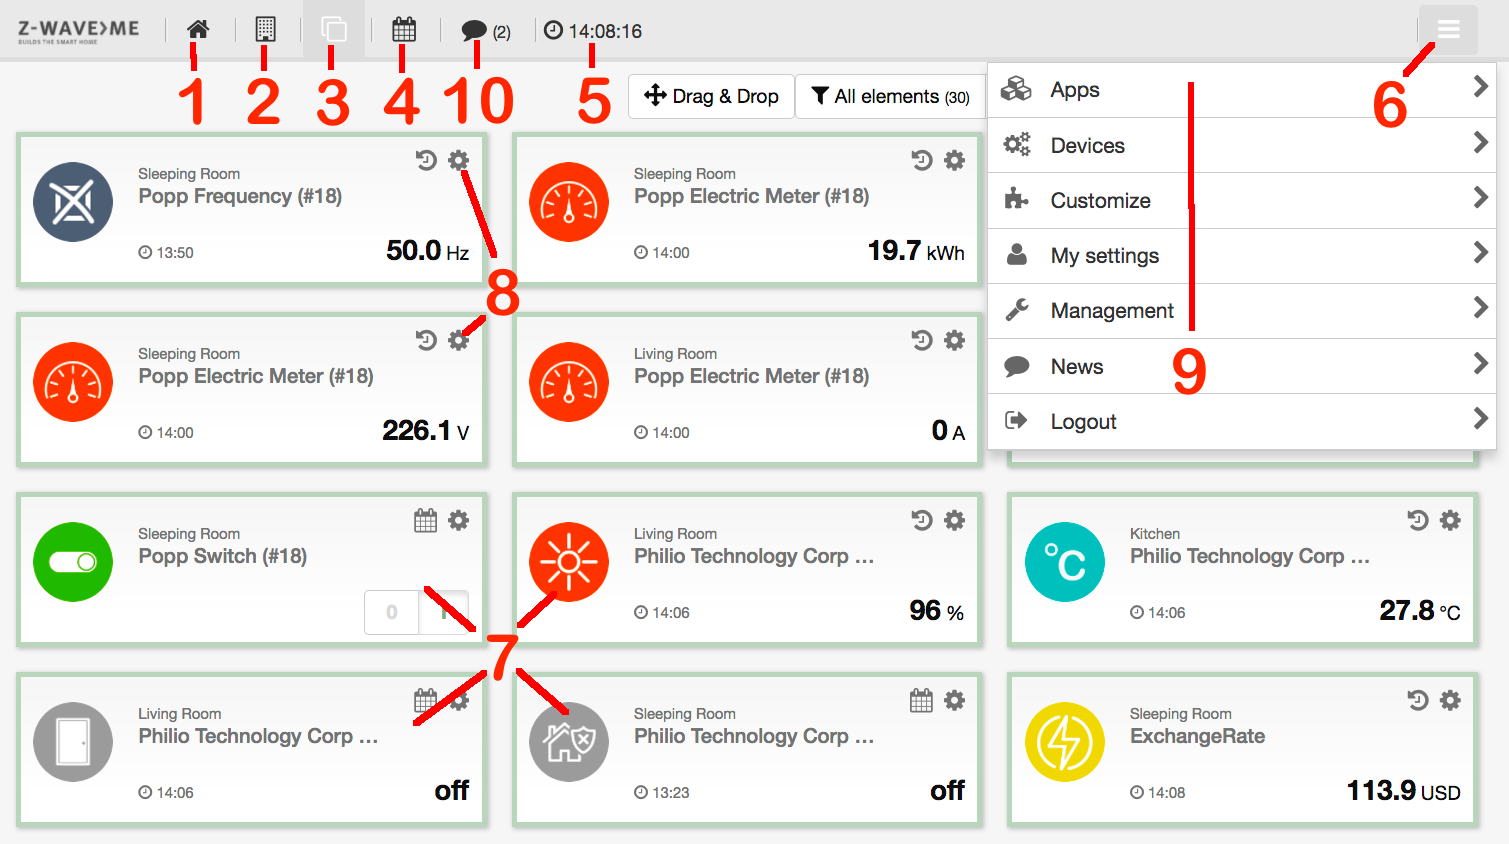
\includegraphics[width=1.0\textwidth]{pngs/cap4/shui1a.png}
\caption{\zwshui}
\label{sh2}
\end{center}
\end{figure}


\section{\zwshui Daily Usage}

 
\subsection{Standard Element View}

Figure \ref{sh2} shows the standard element view of the \zwshui. 
Elements with an icon, buttons, or variables are placed side by side. Depending on the 
screen size, they are grouped in one (mobile phone), two (pad), or three (PC screen) 
columns.

The very same display is available on the \keystroke{Dashboard} (No. 1), the \keystroke{Room View} (No. 2), 
and the \keystroke{Element view} (No. 3). The element view shows all elements (No. 7) available
while the dashboard shows elements that where manually selected for display on the 
dashboard. The clock on the topline menu (No. 5) shows the actual time in the time 
zone of the gateway (not the actual position of the browser). The elements can be filtered 
by element type or can be ordered by

\begin{itemize}
\item Time of creation (ascending or descending)
\item Given name in alphabetical order (ascending or descending)
\item Last update
\item Custom
\end{itemize}

The button \keystroke{Drag-and-Drop} turns the user interface in a reordering mode. Just drag and drop 
elements to reorder them. After the new order is saved, it is available as 'custom'. The 
same logic can be applied to all view showing elements (Element View, Dashboard, and Room 
View).

A search field allows searching for given names of the elements.

All elements can be assigned to ``tags’’: Tags are text blocks that can be arbitrarily 
chosen. Typical tags are ``Temperatures,’’ ``Energy,’’ and ``Outdoor.’’  Multiple elements 
can have the same tag and one element can have several tags. By selecting a tag, only 
elements are shown that are tagged with this name.

Tags are managed on the element configurations described below.

\begin{figure}
\begin{center}
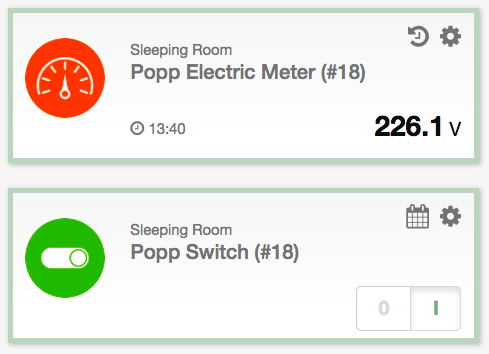
\includegraphics[width=0.4\textwidth]{pngs/cap4/sh4.png}
\caption{Elements}
\label{sh4}
\end{center}
\end{figure}

Figure \ref{sh4} shows two typical elements:
Each element has a given name. This name may refer to the function or the position. Please 
make sure to keep the name short enough so that no display problem is created. Each element 
also has one or several icons. In case the element represents an actor function, the icon 
usually refers to the switching state of the actor (on or off, up or down). Changing icons 
also indicate the status of binary sensors such as motions detectors.
Analog sensors typically only have one icon. The upper element is an actor allowing to 
be switched on and off. 

%Additionally, this element allows changing a color. Clicking on the 
%small triangle right to the word RGB will open a color picking sub-dialog. Above the 
%given name is the room name if the element is assigned to a room.

The 
\includegraphics[width=0.04\textwidth]{pngs/wheel.png} (No. 8 on Figure \ref{sh2}) on 
the right-hand side opens the element configuration dialog. The symbol left to the configuration 
wheel depends on the type of device. For devices with analog values such as rain sensors, 
temperatures, etc., the icon 
\includegraphics[width=0.04\textwidth]{pngs/24hour.png} will 
open a 24-hour history of the sensor value. Devices 
with 24-hour history also show a time stamp when the last value update was received. 
Clicking on the large icon itself will call for a value update, but please keep in mind 
that battery-operated devices will only send updated values after the next wakeup.
For event-driven devices such as actuators or binary sensors, an icon 

\includegraphics[width=0.04\textwidth]{pngs/10events.png}
will show a list 
of the last 10 events with the time stamp. One click away is then the full list of 
events, as described in Section \ref{timeline}, but filtered for this element.

\subsubsection{Element Configuration}
\label{ElementConfiguration}

Every element shown has its own configuration dialog (No. 7 on \ref{sh2}). Clicking 
on the 
\includegraphics[width=0.04\textwidth]{pngs/wheel.png} symbol on the upper right-hand 
side opens this dialog.

\begin{figure}
\begin{center}
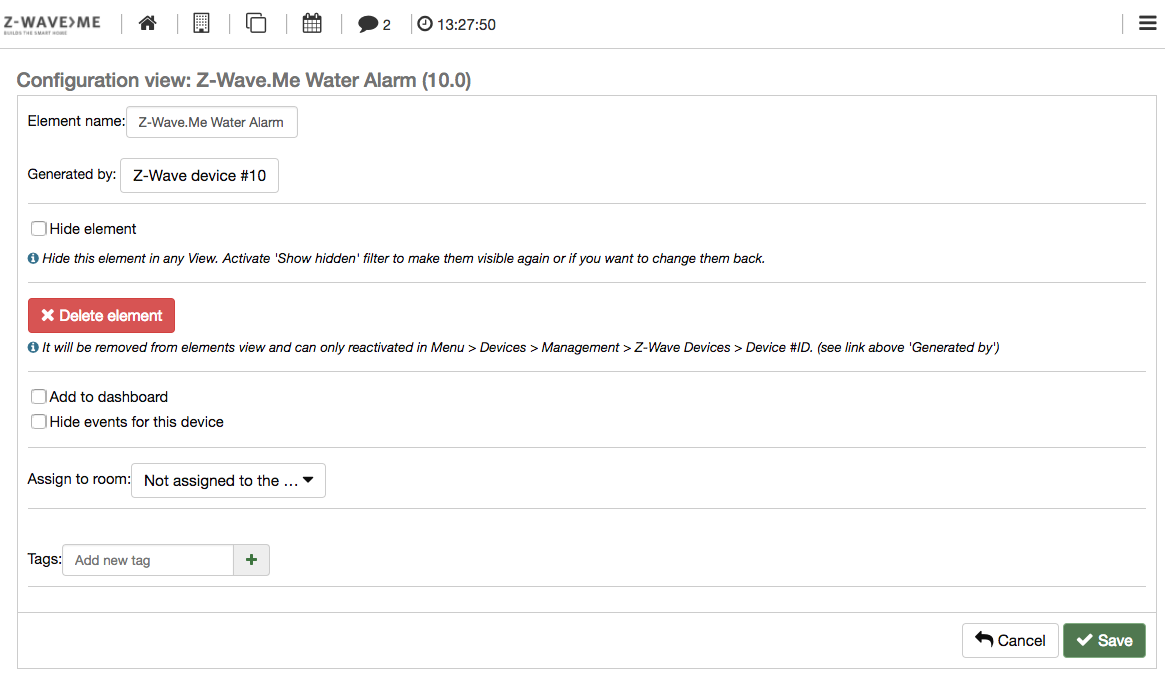
\includegraphics[width=0.9\textwidth]{pngs/cap4/elementconfiguration.png}
\caption{Elements configuration - upper part}
\label{sh5}
\end{center}
\end{figure}

Figure \ref{sh5} shows the upper part of the element configuration dialog.

The element name  is the given name of the element. \zway tries to automatically find a 
reasonable name, but  the user should change this name according to the specific setup of 
the home.

\begin{itemize}
\item Generated By: This refers to the physical device of the \zway application that 
generated this element. In the example above, this device is the physical \zwave device 
with Node ID 2. Clicking on the button with the name of the element-creator leads to the 
configuration dialog of the physical device, i.e. the \zway application.

\item Hide element: As explained in the dialog, this checkbox will hide the element. However, 
this setting can be reversed by showing hidden devices. This setting is for cosmetic view only.

\item Delete Element: This checkbox allows removing the element. It will not only disappear 
from the element view but also from any dropdown list to setup device relationships, etc. 
For information on how to re-activate such an element, refer to the user settings dialog 
description in Section \ref{mysettings}.

\item Add to Dashboard: This places the element on the dashboard.

\item Hide events from this device: This keeps the device in the element view or Dashboard, but 
no events of this device will be shown in the event timeline.

\item Assign to room: This allows assigning this element to a certain room or changing 
this assignment.

\end{itemize}

\begin{figure}
\begin{center}
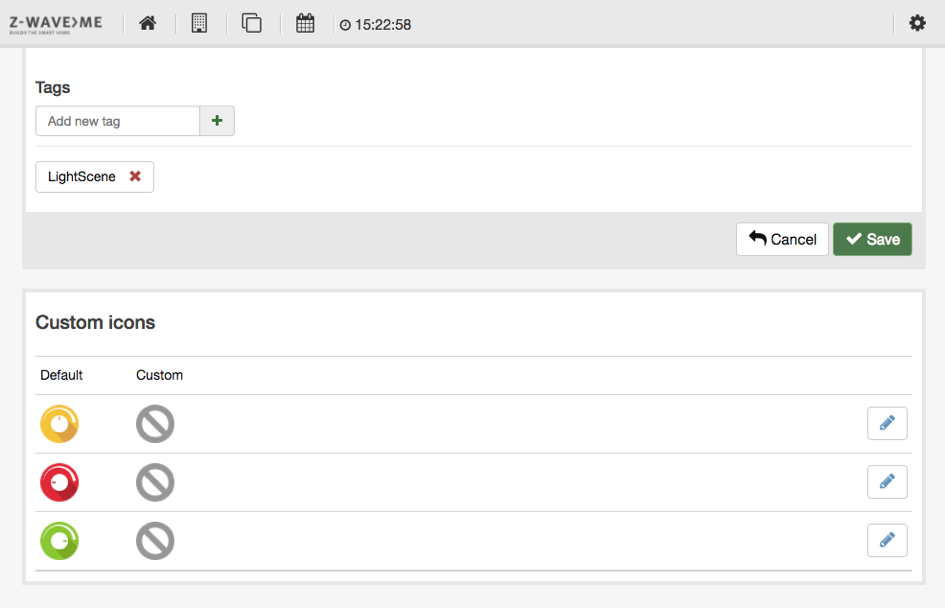
\includegraphics[width=0.9\textwidth]{pngs/cap4/sh6.png}
\caption{Elements configuration  - lower part}
\label{sh6}
\end{center}
\end{figure}

Figure \ref{sh6} shows the lower part of the element configuration dialog. The tag option 
allows setting and removing tags. When a tag name is inserted into the text field, it 
autocompletes known tag names.

The custom icon sub-dialog allows changing the icons of the element. Each element has one, 
two, or three icons depending on the status indicated. Each of the icons can be replaced 
by an own individual icon. Just click on the pencil button to change the icon. To 
download more icons, refer to the customization section in the configuration menu.

\subsubsection{Room View}
\index{Rooms}

The \zwshui allows managing different rooms and assigning elements to 
rooms. Each element can be placed in one room only.

Clicking on the room symbol on the top menu opens the room view with a list of rooms, 
as shown in Figure \ref{roomover}.

\begin{figure}
\begin{center}
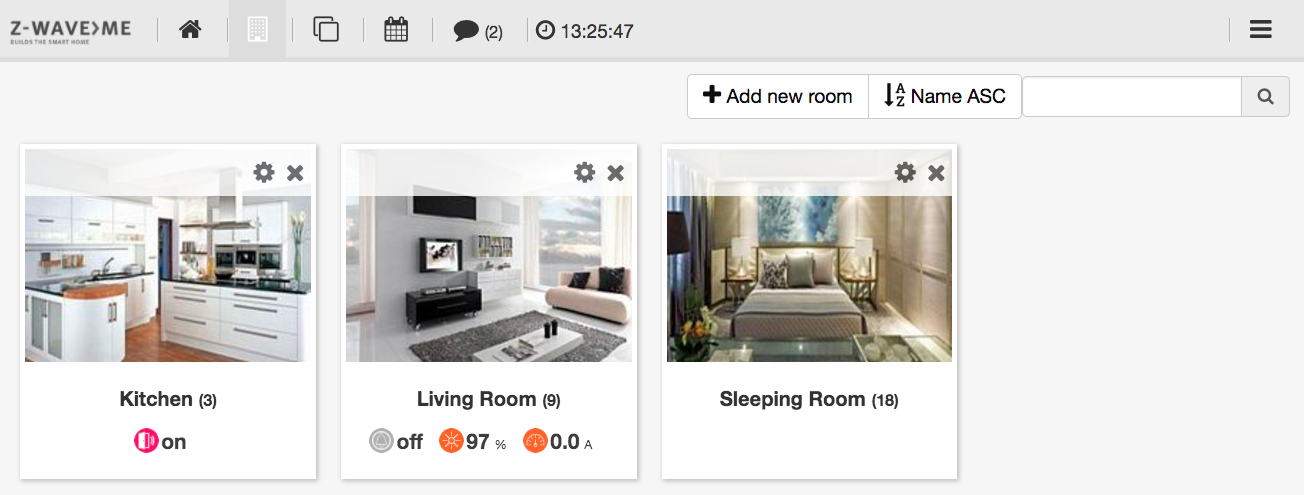
\includegraphics[width=0.9\textwidth]{pngs/cap4/roomover.png}
\caption{Room overview}
\label{roomover}
\end{center}
\end{figure}

Each room has its own element with a background image that can be configured. It is 
possible to add new rooms using the button labeled \keystroke{Add room}.
The room is named and the number of elements in this room is shown. Per room there 
are up to three sensors that can be selected as ``quick-view sensors’’. They are shown 
right below the name and in the top menu in the individual room view.

Clicking on the room element leads to the room view, as shown in Figure \ref{roomview}.

\begin{figure}
\begin{center}
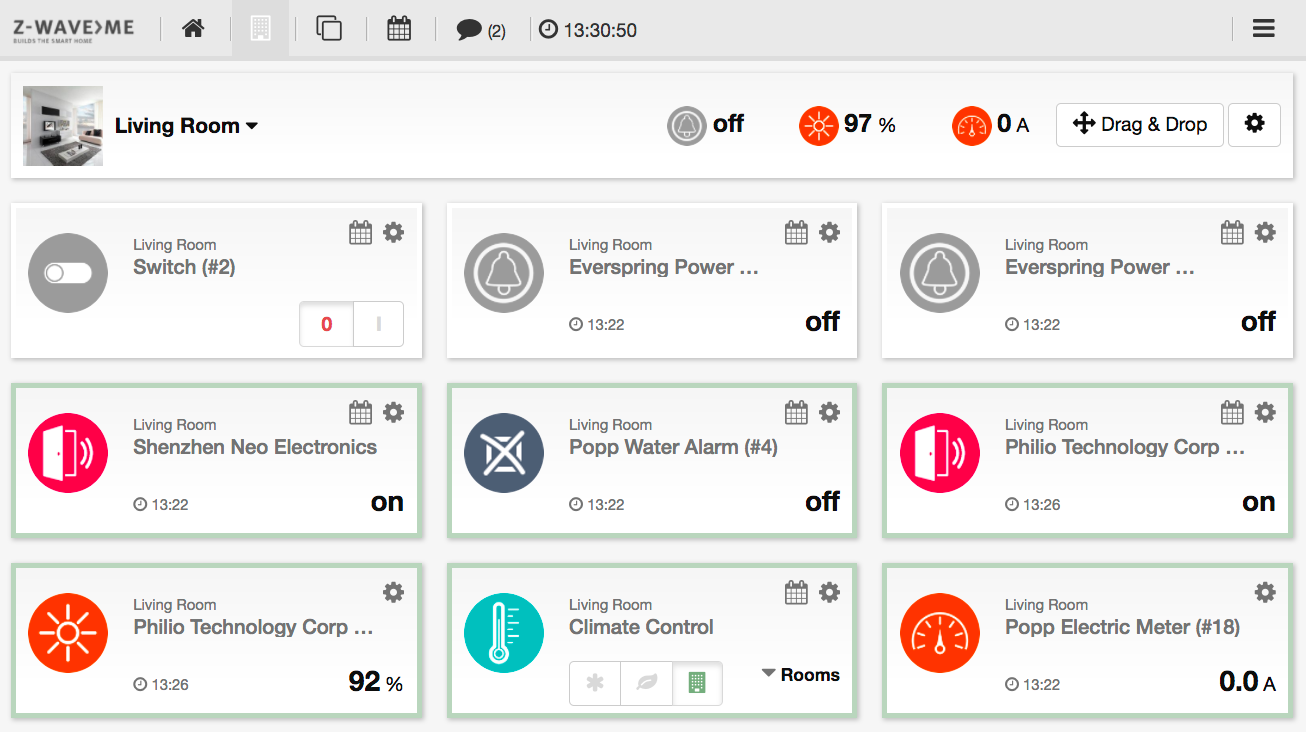
\includegraphics[width=0.9\textwidth]{pngs/cap4/roomview.png}
\caption{Room View}
\label{roomview}
\end{center}
\end{figure}

The room view lists all the elements in the room. As in the element view, they can be 
re-arranged using the drag-and-drop feature.

The top line shows up to three quick sensors and allows quick change of the room using 
the dropdown list. If your browser supports gestures, you can change the rooms by 
swiping left or right.

Clicking on the 
\includegraphics[width=0.04\textwidth]{pngs/wheel.png} symbol of the 
room element or inside the room view in the top line opens the room configuration 
dialog, as shown in Figure \ref{sh7}.

\begin{figure}
\begin{center}
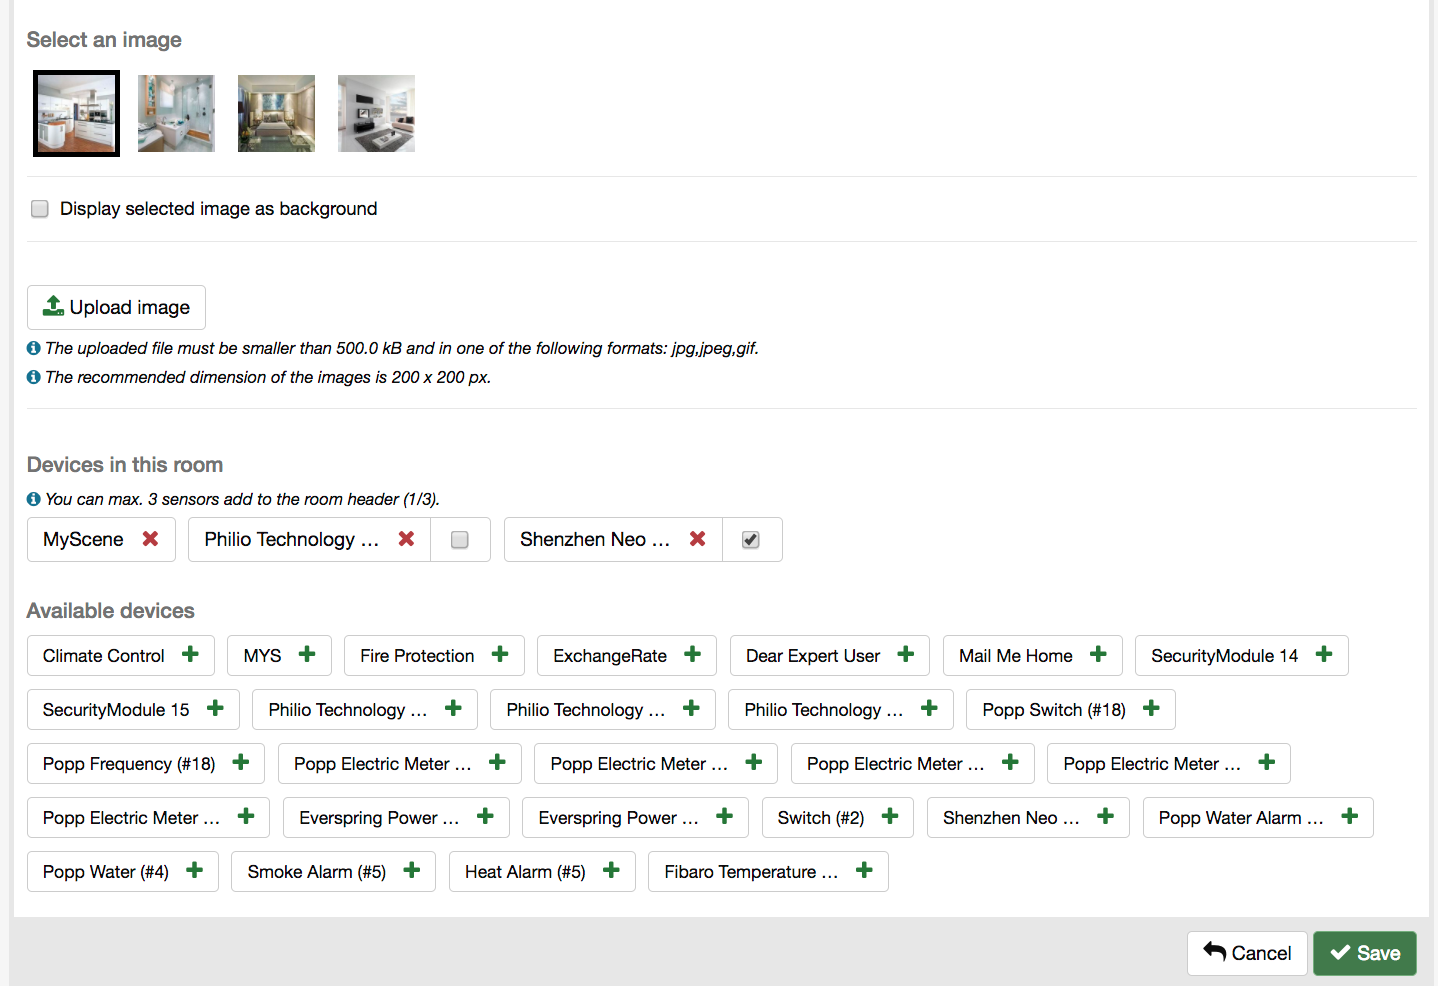
\includegraphics[width=0.9\textwidth]{pngs/cap4/sh7.png}
\caption{Room configuration dialog}
\label{sh7}
\end{center}
\end{figure}

Each room can have an individual name. Besides some pre-installed images, it is possible 
to upload images for the room. A checkbox defines the room image that is used as a 
background image in the room view.

The dialog allows assigning elements to this room which were not assigned to any room 
yet. Just click on the element name in the list of \keystroke{Available devices}.

The little checkbox on the right-hand side allows selecting up to three sensors as 
``quick-view sensors’’.

\subsubsection{Event Timeline}
\label{timeline}

The event timeline is the forth menu item in the top menu.

\begin{figure}
\begin{center}
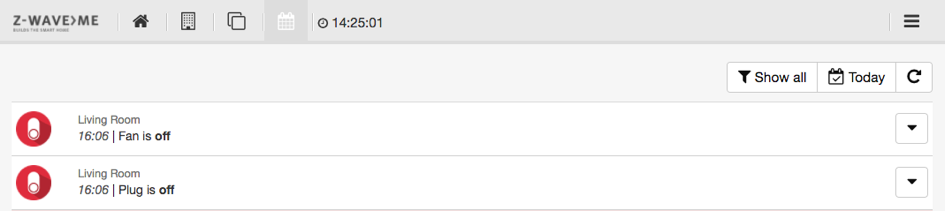
\includegraphics[width=0.9\textwidth]{pngs/cap4/sh8.png}
\caption{Timeline}
\label{sh8}
\end{center}
\end{figure}

The timeline dialog offers a chronological view of the events in the Smart Home. The events 
are:

\begin{itemize}
\item Change of status of actuators such as dimmers, blind controls, or switches
\item Tripping of binary sensors (motion, door, etc.)
\item Change of measured value of sensors
\item Network status changes (device lost, device back, etc.)
\end{itemize}

The standard view of the timeline, as shown in Figure \ref{sh8}, lists all events with the 
icon of the element, room info, time stamp, name of the element, and status info. Every 
line item has a context menu on the right-hand side. This menu allows

\begin{itemize}
\item showing events of this source element only,
\item showing events of this event type only,
\item showing events that have the same event type,
\item directly moving to the element configuration page of this element,
\item hiding all events from this source.
\end{itemize}

\subsection{News feed}
\index{News Feed}

 Each \zway controller is connected to an RSS feed. This feed contains news and alerts 
 about the platform. Whenever there is a new feed entry, the top menu bar will indicate 
 this with a sign, as shown with Marker 1 in Figure \ref{news1}. Clicking on this opens 
 the full list of news. This full list can also be accessed using the 'News' menu 
 item in the configuration section, as described in Section \ref{news}.

\begin{figure}
\begin{center}
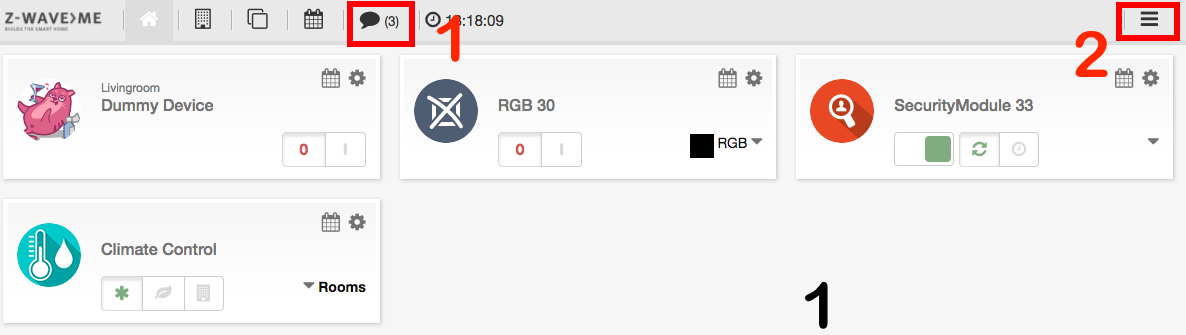
\includegraphics[width=0.9\textwidth]{pngs/cap4/news1.png}
\caption{News Indicator}
\label{news1}
\end{center}
\end{figure}

\section{The Configuration Menu}

Clicking on the menu item (marked as No. 2 in Figure \ref{news1}) on the right-hand side 
opens the configuration menu. The configuration offers various functions to enhance and 
configure the smart home system as such and the user interface. Figure \ref{sh9} shows the configuration menu of \zway.

\begin{figure}
\begin{center}
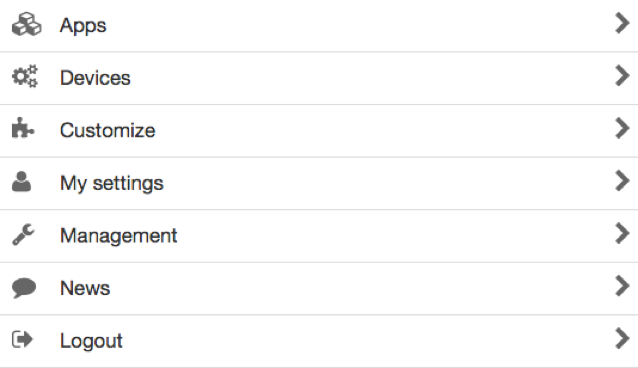
\includegraphics[width=0.9\textwidth]{pngs/cap4/sh9.png}
\caption{Configuration menu}
\label{sh9}
\end{center}
\end{figure}



\subsection{Apps}
\label{appssetup}
\index{Apps}

This menu option allows managing the home automation applications and interfaces of 
Internet or IP-based services or devices.

\zway apps are like software applications that use the infrastructure of the \zwave 
network to provide application solutions and dependencies. These software applications also 
extend the capabilities of the network and implement automation functions.

\begin{figure}
\begin{center}
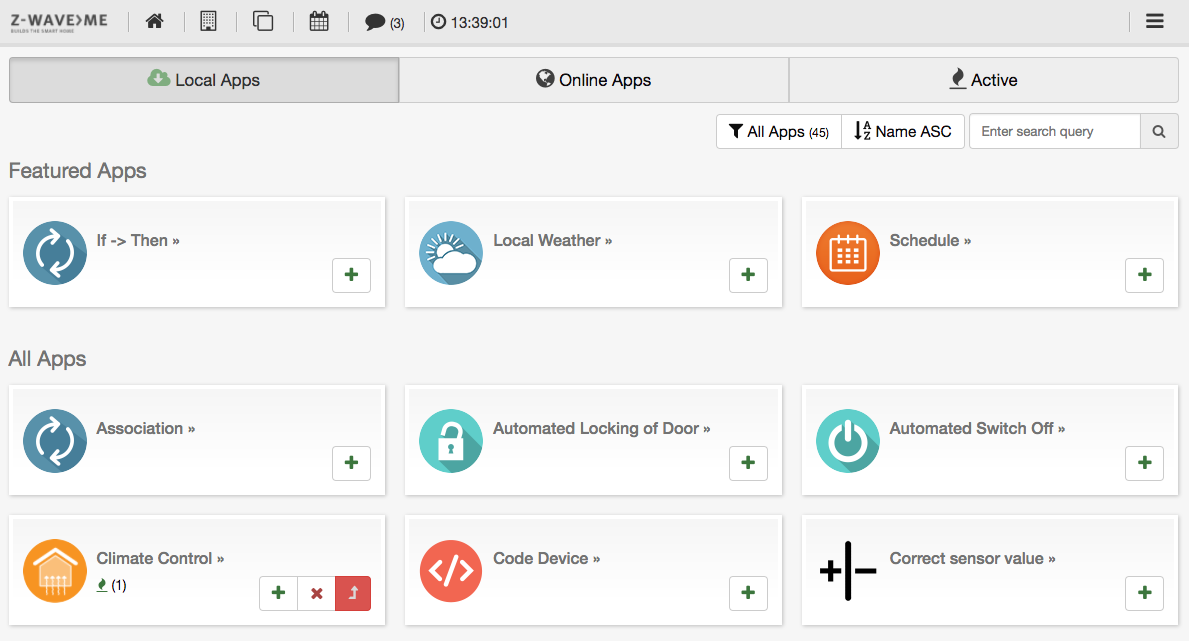
\includegraphics[width=0.9\textwidth]{pngs/cap4/app2.png}
\caption{Local Apps}
\label{app2}
\end{center}
\end{figure}

Like any other application software such as those for PCs, some \zway apps are preinstalled 
on the device, and others can be downloaded and installed by the user. Like application 
software, some software solutions can only run once while others can be started multiple times.


\begin{figure}
\begin{center}
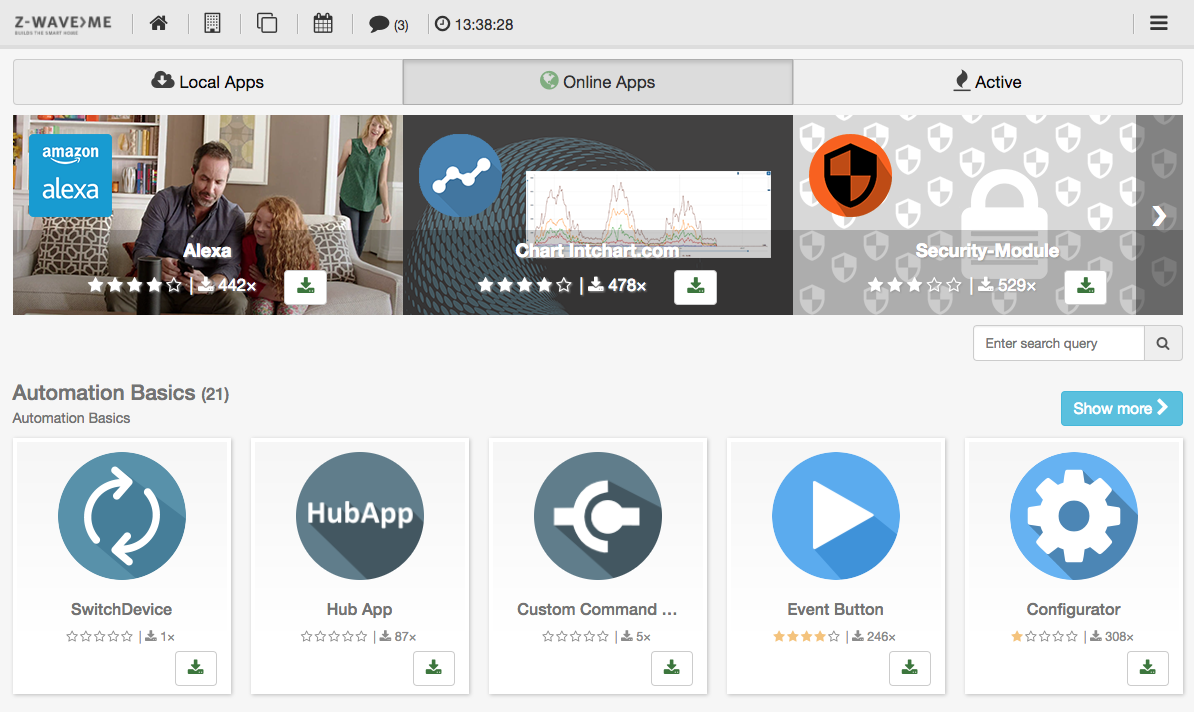
\includegraphics[width=0.9\textwidth]{pngs/cap4/app1.png}
\caption{Online Apps}
\label{app1}
\end{center}
\end{figure}

The app menu has three parts:

\begin{itemize}
\item List of apps locally available for use.
\item List of apps available on the central server and ready for download.
\item List of apps that are active and running.
\end{itemize}

The list of local apps, as displayed in Figure \ref{app2}, shows a small subset of apps that 
are already on the local devices. The top part shows some of the apps that are most 
frequently used (featured apps). A filter allows filtering for certain app types; 
ordering and direct search in the search box also help to find the right app. If 
there are active instances of the app (software running x times with different
 parameters), this is indicated right below the name of the app.

\begin{figure}
\begin{center}
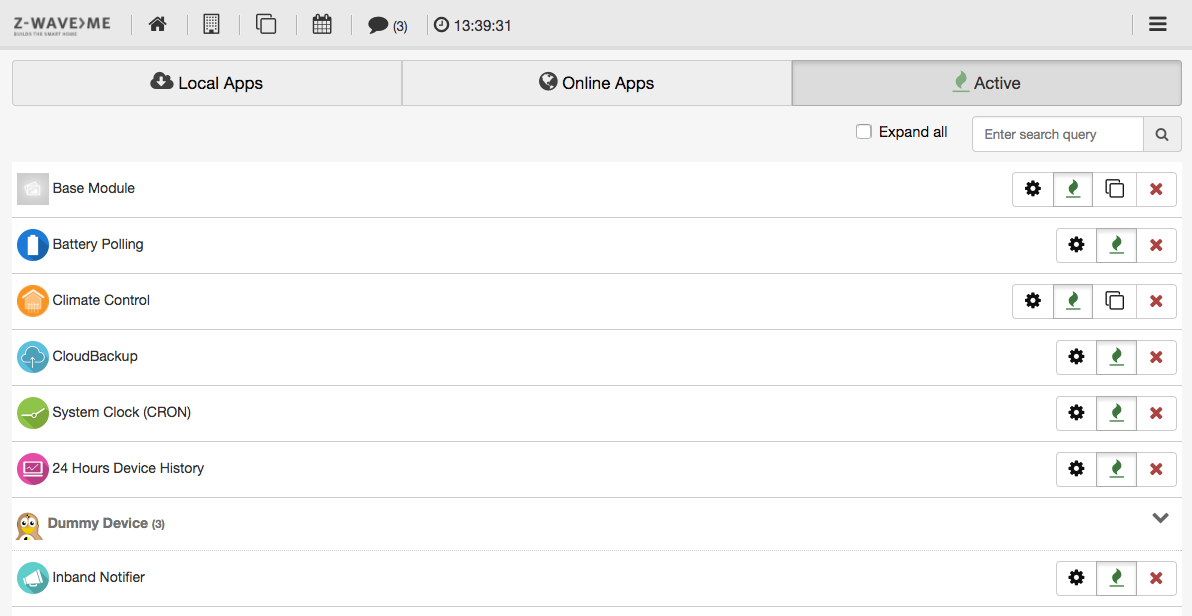
\includegraphics[width=0.9\textwidth]{pngs/cap4/app3.png}
\caption{App Setup}
\label{app3}
\end{center}
\end{figure}

Clicking on the name will open a dialog with further information about the app. Clicking 
on the \keystroke{+} button will lead right to the configuration page of the app.

The online app list, as shown in Figure \ref{app1}, offers the same functions. However, 
apps need to be downloaded first before they can be configured and started. Clicking on 
the download button will copy the app to the local repository and start the configuration 
dialog, as shown in Figure \ref{app3}.

Each app has its own name that can be changed. Depending on the function of the app, 
there are several different setup parameters.

\textbf{Please note again that some apps can be started multiple times while other 
apps are ``singletons.’’ They must only run once on the system. Once they run, they 
will disappear from the repository since they cannot be started again. Configuration
 of such a singleton is still possible using the menu of running apps. If such an app 
 stops, the app entry will reappear in the local repository.}

\begin{figure}
\begin{center}
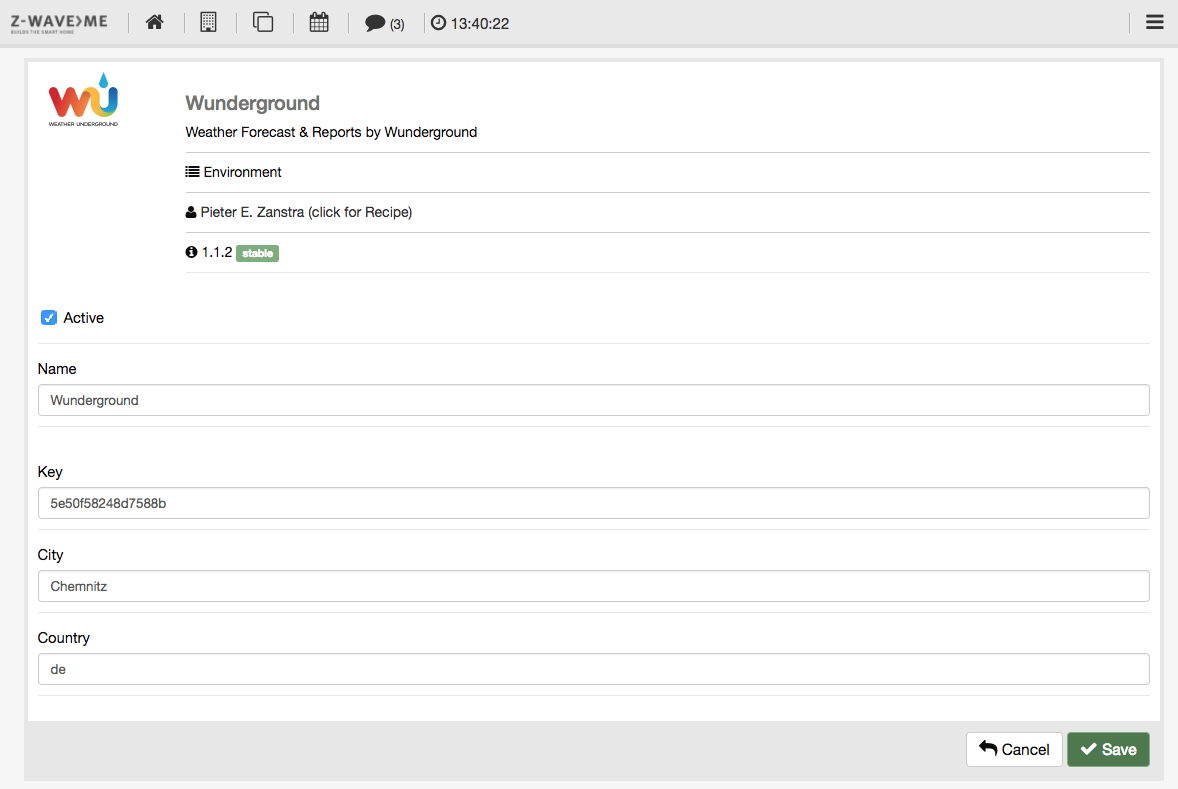
\includegraphics[width=0.9\textwidth]{pngs/cap4/app4.png}
\caption{Active App Management}
\label{app4}
\end{center}
\end{figure}

The tab for active app management is shown in Figure \ref{app4}. It lists all active 
apps by app type. If there are more than one app of the same type (e.g. \app{IF->THEN} is 
usually needed multiple times), the view is collapsed for this type of application but 
can be expanded. It is possible to expand all sections of multiple app types using the 
checkbox on the top. It is also possible to search for certain app names.

Every app line has a submenu with the following functions:

\begin{itemize}
\item 
\includegraphics[width=0.04\textwidth]{pngs/redcross.png}: Stop this app
\item 
\includegraphics[width=0.04\textwidth]{pngs/double.png}: Allows cloning an app. This will open a dialog for a new instance of the 
same app with the same settings. After saving these settings, the new app becomes active 
and is shown in the list too.
\item 
\includegraphics[width=0.04\textwidth]{pngs/greenflame.png}: Stop the App. It remains configured but is inactive. Once inactive, 
the green flame changes into a red ON button to restart the app.
\item 
\includegraphics[width=0.04\textwidth]{pngs/wheel.png}: Opens the configuration dialog. This is the very dialog to be completed 
during the initial start of the app.
\end{itemize}

Please refer to Chapter \ref{apps} for more information on different apps.

\subsection{Devices}
\index{Devices}

\begin{figure}
\begin{center}
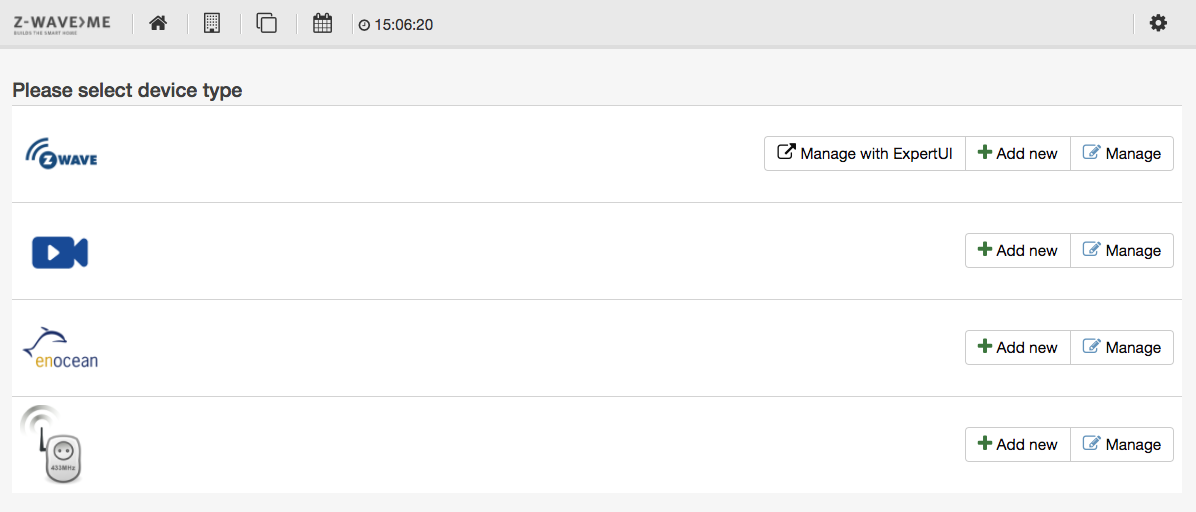
\includegraphics[width=0.9\textwidth]{pngs/cap4/433_5.png}
\caption{Device Management Overview}
\label{device0}
\end{center}
\end{figure}


The device menu allows managing physical devices. By default, it offers two physical 
device types: ``\zwave devices’’ and ``IP cameras.’’ However, if other wireless communication 
technologies are activated, they will be shown as well. Please refer to 
Chapter \ref{extensions} for more information on how to integrate further 
wireless technologies.   This section will also explain how to include/exclude and manage 
these devices and IP cameras.

Figure \ref{device0} shows the device list including EnOcean and 433 MHz devices.

Therefore, let us focus here on managing \zwave devices. Besides the standard buttons 
to add and manage devices of the specific communication technology, \zwave offers one
 more button to link to a specific second \zwave user interface for installers and professionals.
Please refer to Chapter \ref{expertuserinterface} for a detailed description of this very 
technical, the so-called \zweui. Please note that all day-to-day management functions 
can be done without involving this very specific and technical interface.

In case the controller hardware supports the new Smart Start feature of \zwave, there will be 
another button to include new devices - the QR code san as sown in Figure \ref{shui-ss1}.

\begin{figure}
\begin{center}

\includegraphics[width=0.9\textwidth]{pngs/cap4/shui-ss1.png}
\caption{Scan QR Code for Smart Start}
\label{shui-ss1}
\end{center}
\end{figure}

Smart Start is a new way to include devices into Z-Wave using the QR code 
provided with S2 authentication.  The user scans the QR code thats is stored in an internal 
so called  provisioning list. Smart Start Devices will then announce to be included when 
powered up. In case the S2 key is in the provisioning list the controller will automatically 
include  this new device without any further user interaction.

The button 'QR Code' opens a dialog to capture the Device Key, either by 
typing them in or by scanning the QR. Another menu tab allows managing the Device Keys 
already captured by not used for inclusion.

Please note that a standard
web browser running on a standard PC may not provide the capability to scan QR codes.


\subsubsection{Inclusion}
\label{inclusion}
\index{Inclusion}
\index{Exclusion}

\begin{figure}
\begin{center}
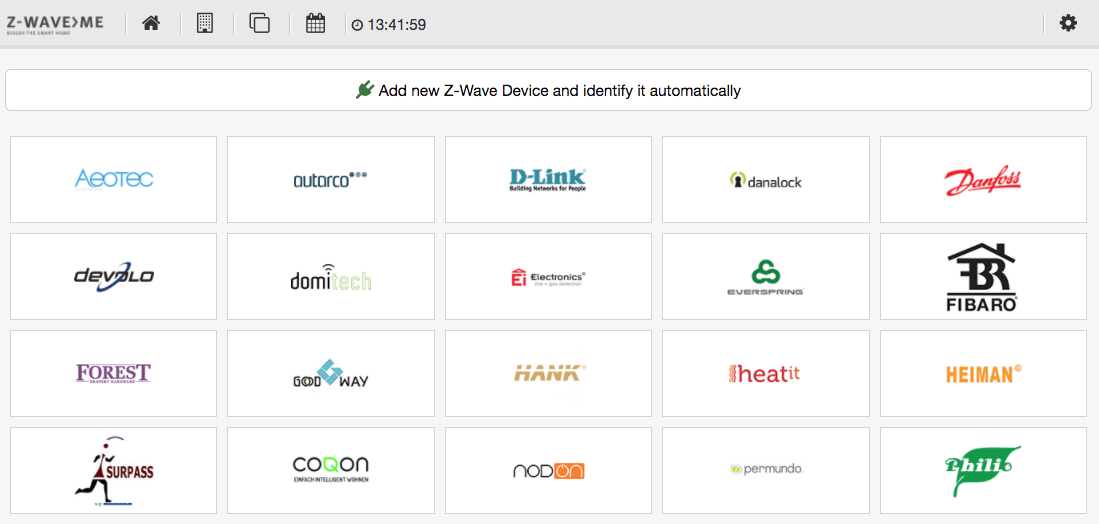
\includegraphics[width=0.9\textwidth]{pngs/cap4/device1.png}
\caption{\zwave Device Vendor Overview}
\label{device1}
\end{center}
\end{figure}

To include a new \zwave device (one of the first steps needed to start a smart home 
system!) please click on the \keystroke{+} button on the \zwave device part. This will open an 
overview of current \zwave device vendors by name and logo. Figure \ref{device1} 
shows this overview.

Generally, there is no need to know the \zwave brand and product code. All \zwave devices 
are self-describing, and automatically identified products will provide the same functions 
as the devices that were pre-identified. Thus, experienced users will always click on 
the upper button to add a new unidentified \zwave device. The only reason to find a 
specific device from the list is to get some additional information on how to include this 
device. This refers to the button and the button push sequence needed for inclusion.

Since most \zwave devices have one \zwave inclusion button and single or triple click 
will do the inclusion, this information is only needed for some devices with exotic 
inclusion options. Both the buttons to include an unknown device and the right-hand 
side button of an identified button will lead to the same inclusion dialog as 
shown in Figure \ref{device3}.

\begin{figure}
\begin{center}
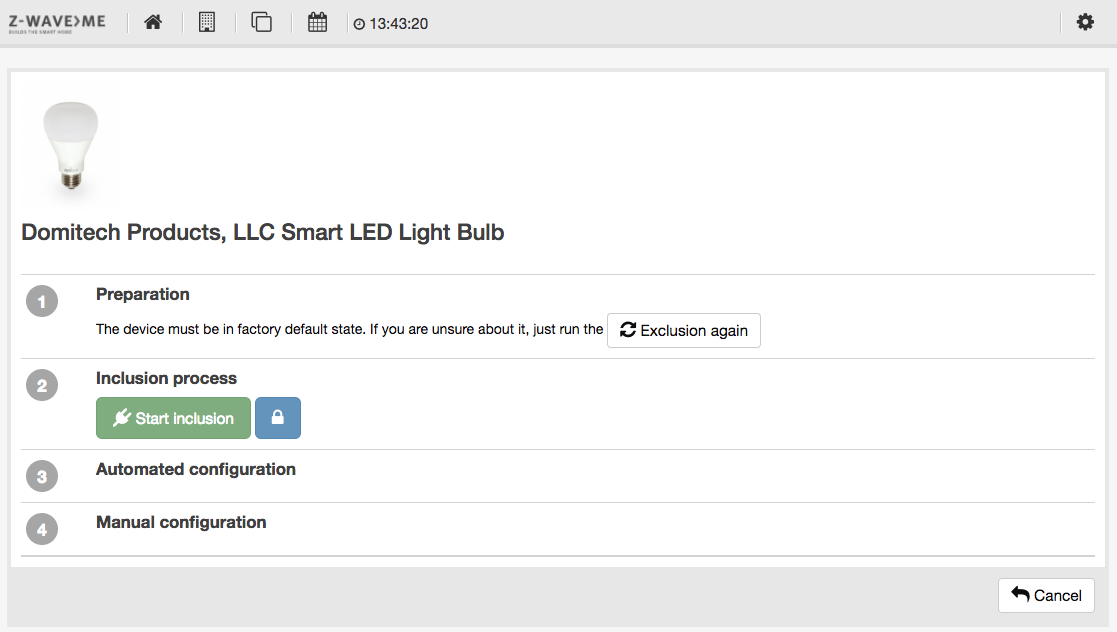
\includegraphics[width=0.9\textwidth]{pngs/cap4/device3.png}
\caption{\zwave Device Inclusion Dialog}
\label{device3}
\end{center}
\end{figure}

\vspace{5mm}
\noindent\framebox{\noindent
\begin{minipage}{\dimexpr\linewidth-2\fboxrule-2\fboxsep\relax}
\begin{center}
{\fontsize{20}{28}\selectfont It is recommended to exclude (reset) a device before it gets included.}
\end{center}
\end{minipage}}
\vspace{5mm}

However, 
if you are sure that the device is new and in factory default state, you may skip this 
step. Right next to the inclusion button there is another small button that defines if the 
device will be included with special security functions. By default, the security option 
is enforced. However, some devices in the market may not work as expected using the 
security function. In case there is a connection problem, unsecure inclusion may still work.

Once the inclusion mode has been started, the controller waits for devices to be 
included. Figure \ref{incl1} shows the controller at this moment. The inclusion mode can 
be terminated using the same button. Any new device included will also terminate the process.

\begin{figure}
\begin{center}
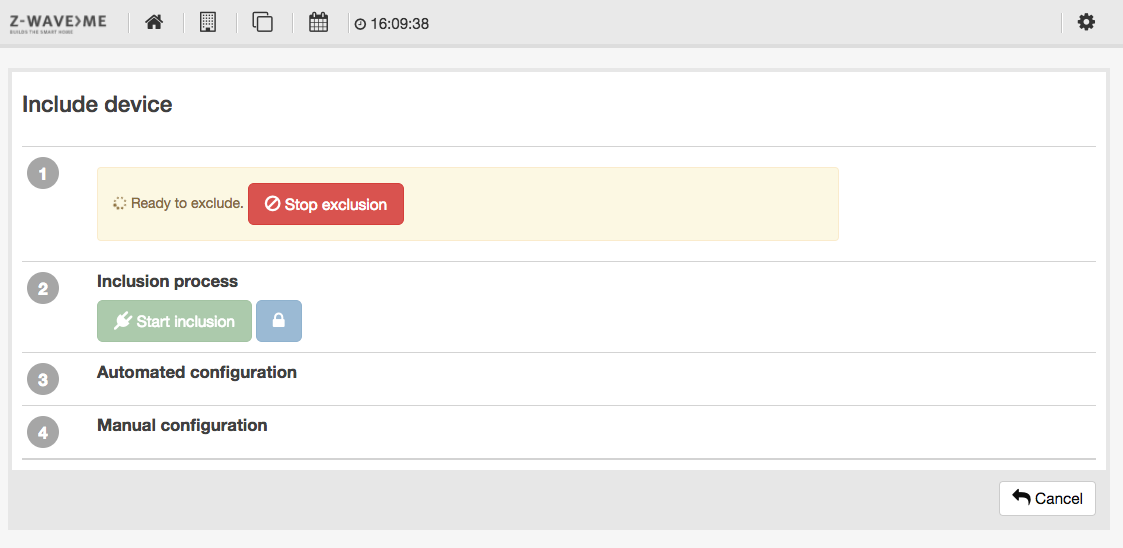
\includegraphics[width=0.9\textwidth]{pngs/cap4/incl1.png}
\caption{\zwave Device Exclusion Dialog}
\label{incl1}
\end{center}
\end{figure}

\begin{figure}
\begin{center}
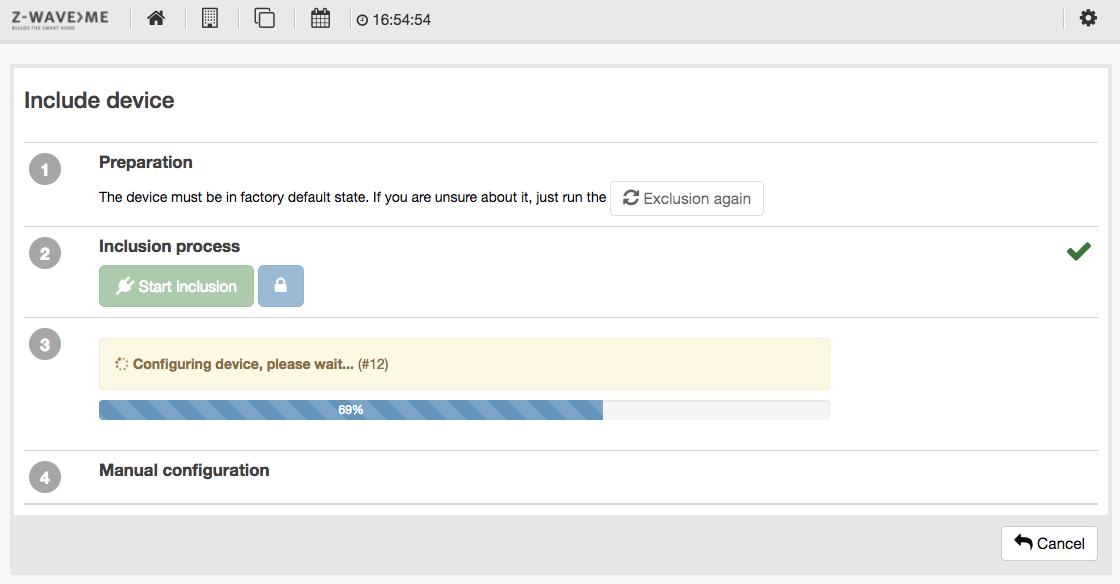
\includegraphics[width=0.9\textwidth]{pngs/cap4/incl2.png}
\caption{\zwave Device Successful Inclusion}
\label{incl2}
\end{center}
\end{figure}

In case the new device requires authorization, this needs to be done 
right after inclusion.
Authorization ensures that the device that appears on the user interface is indeed the 
device in hand. To ensure this the device offers either a QR code to be read or a 
device individual PIN number, both types of information need to be provided to the user 
interface manually.
The controller will then match the information provided by the user with the information 
provided by the device using wireless communication. Only in case they match the device 
can be used.

\begin{figure}
\begin{center}
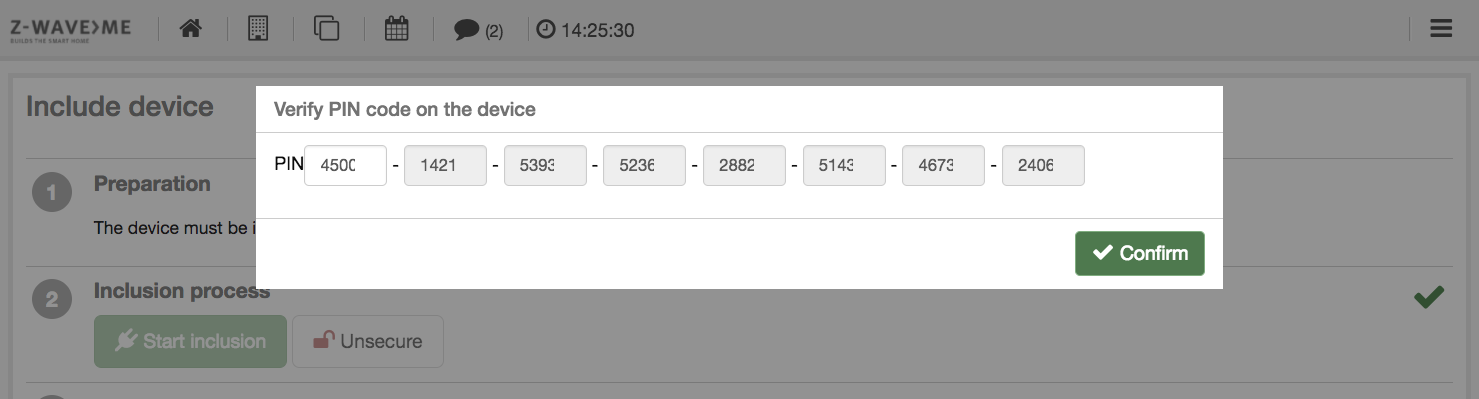
\includegraphics[width=0.9\textwidth]{pngs/cap4/SHUI_S2AUTH.png}
\caption{\zwave Device Authentication}
\label{security2_6}
\end{center}
\end{figure}

Authentication is only required for certain devices. In this case, a 
window like that shown in Figure \ref{security2_6} pops up asking for the authentication 
information. Once given, they are checked. If authentication fails, a warning is 
displayed. It is not possible to just repeat the authentication. The 
device must be excluded and re-included.


Any new device will be interviewed next. In this process, all functions announced by 
the device itself will be verified and certain user interface relevant data will be called 
from the device. A progress bar such as that in Figure \ref{incl2} shows the status.

Once the interview was passed successfully, a dialog offers some initial manual configuration 
functions, as shown in Figure \ref{device3}:

\begin{figure}
\begin{center}
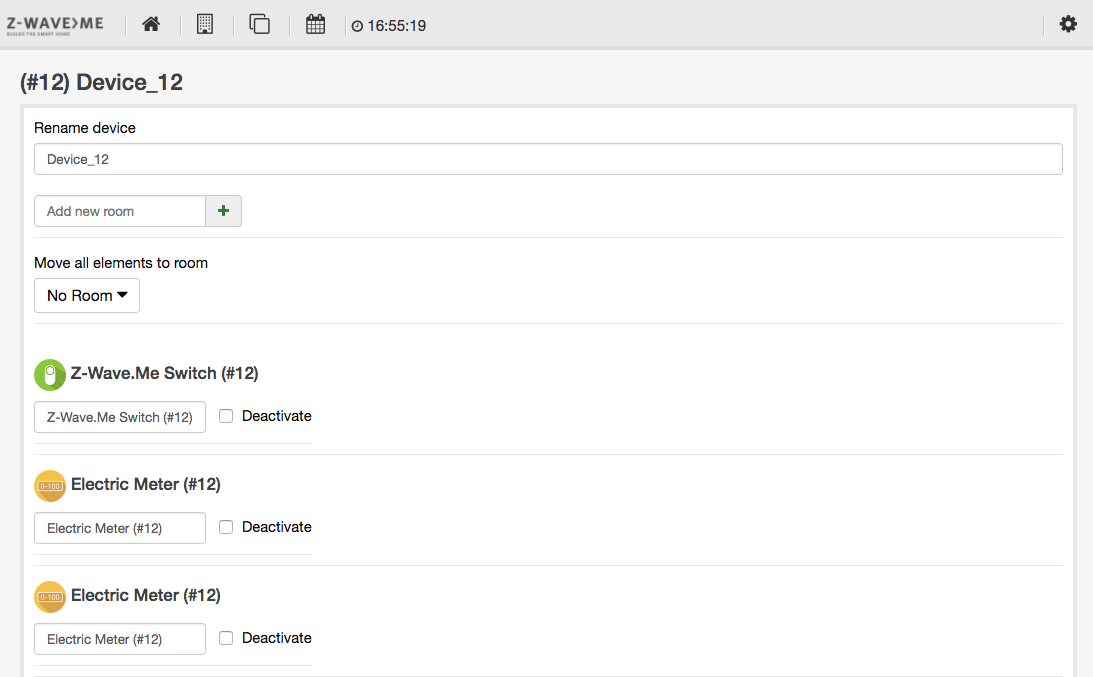
\includegraphics[width=0.9\textwidth]{pngs/cap4/incl3.png}
\caption{\zwave Device manual configuration}
\label{incl3}
\end{center}
\end{figure}

\begin{itemize}
\item Rename the device as such. This device name only refers to the physical device and 
will not be shown in the standard user interface. Use descriptive words 
like ``Popp Smoke on sealing’’ to re-identify the device later.
\item It is possible to move all elements shown below into one single room. If this is not 
done here, it is still possible to move each element on the configuration dialog as 
described in Section \ref{ElementConfiguration}.
\item The list of the elements generated by the new device. Here you can change the name 
that will then appear on the element overview, etc. You can also deactivate the element 
if you don’t see any need to have it.
\item Some physical devices offer further hardware-specific settings such as wakeup interval 
time. If the new device offers such configuration, another button for hardware 
configuration is shown. Please refer to the \zweui 
configuration description in Chapter \ref{Configuration} for more information on how to 
use this dialog. Both dialogs are identical.
\end{itemize}

\begin{figure}
\begin{center}
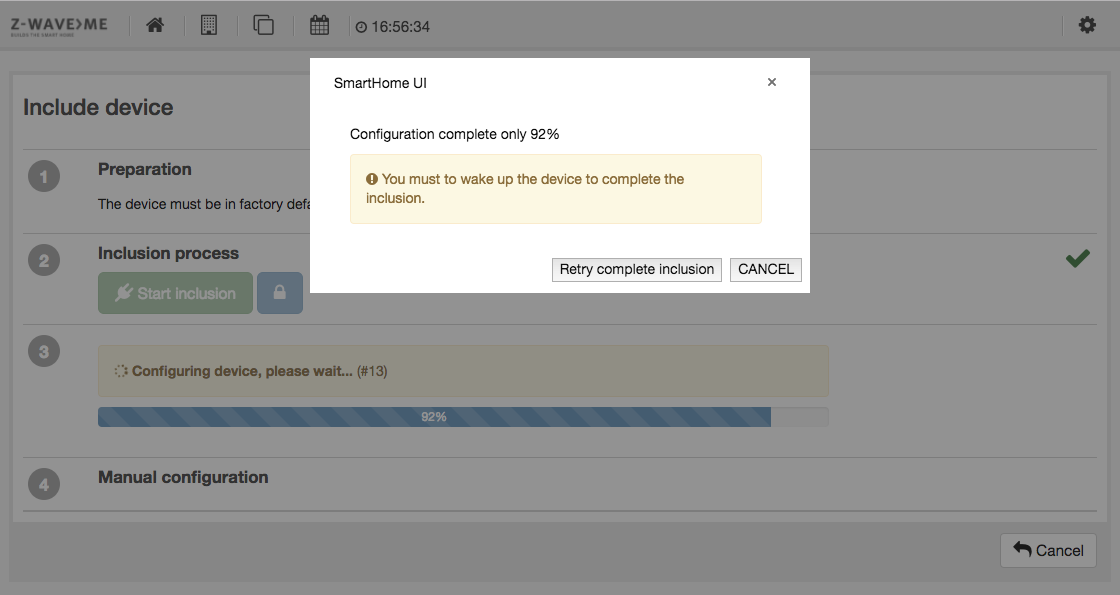
\includegraphics[width=0.9\textwidth]{pngs/cap4/incl4.png}
\caption{\zwave device inclusion failed}
\label{incl4}
\end{center}
\end{figure}

The interview process does not only detect all information from the device; it also tests 
the connectivity of the device. Certain communication may fail. Another good reason for 
such a failure is that a battery-operated device goes into deep sleep mode too fast. 
Figure \ref{incl4} shows the error message in case of failure. In most cases, it’s OK to 
just redo the interview and wake up the device.

If the second attempt at the interview fails, the controllers gives the option to 
accept the result or to redo the entire process. Figure \ref{incl5} shows this dialog box.

\begin{figure}
\begin{center}
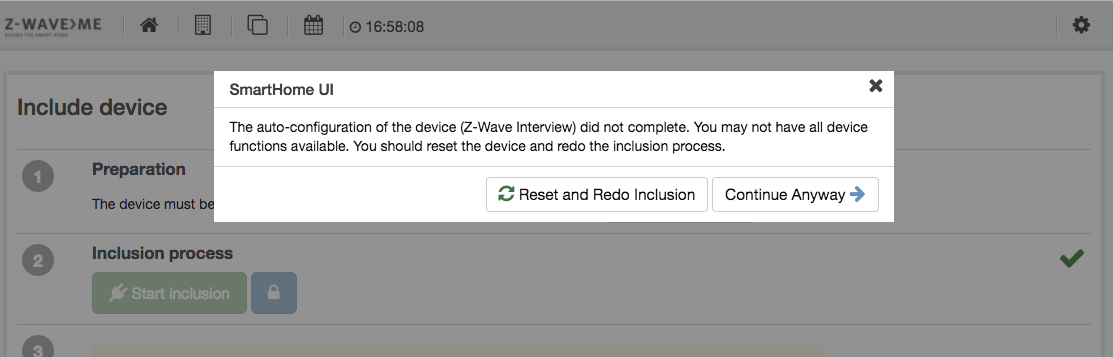
\includegraphics[width=0.9\textwidth]{pngs/cap4/incl5.png}
\caption{\zwave device inclusion repeated}
\label{incl5}
\end{center}
\end{figure}

Once the interview has passed and all configurations are done, the device can be used.

\subsubsection{\zwave Device Management}

The second option for \zwave devices besides adding (including) new devices is the device 
management menu. Clicking on the button \keystroke{Manage} button opens a menu with three tabs:

\begin{itemize}
\item Figure \ref{incl6} shows a list of the physical \zwave devices. The \keystroke{*} button 
will open the very same device management dialog as described during manual post-inclusion 
configuration in Section \ref{inclusion}. The \keystroke{x} button opens a dialog to remove 
the device. As shown in Figure \ref{incldr} there are two options:
\begin{itemize}
\item Reset and Remove: This button will start the normal Z-Wave Exclusion Process. Exclusion
requires that the device to be excluded is still functioning and accessable.
\item Remove: Only in case the device is defect nor not existent anymore this option shall be used.
It will use the Z-Wave function 'Remove Failed Node' without any involvement of the device to be removed.
\end{itemize}
\item Figure \ref{incl7} shows the battery status overview. The list can be ordered by 
the battery charging level.
\item Figure \ref{incl8} shows a list of network status messages. This can be warnings 
for empty battery, devices lost, devices replaced, etc. Clicking on the device name 
lists all the elements created by this physical device.
\end{itemize}


\begin{figure}
\begin{center}
\includegraphics[width=0.9\textwidth]{pngs/cap4/incl6.png}
\caption{\zwave device overview}
\label{incl6}
\end{center}
\end{figure}

\begin{figure}
\begin{center}
\includegraphics[width=0.9\textwidth]{pngs/cap4/incl7.png}
\caption{\zwave device battery overview}
\label{incl7}
\end{center}
\end{figure}

\begin{figure}
\begin{center}
\includegraphics[width=0.9\textwidth]{pngs/cap4/incl8.png}
\caption{\zwave device network status}
\label{incl8}
\end{center}
\end{figure}

\begin{figure}
\begin{center}
\includegraphics[width=0.9\textwidth]{pngs/cap4/devicereset.png}
\caption{\zwave Device Reset /Exclusion}
\label{incldr}
\end{center}
\end{figure}

\subsection{Customize}
\label{customize}


The customization menu option allows changing the look and feel of your \zway user 
interface. You can add more icons as device-specific icons and you can change the look 
and feel using skins. For more information on skins and how to create them, please refer 
to Chapter \ref{MakeSkins}. This menu here only deals with skins that are already available.

The menu offers four tabs. The tab shown in Figure \ref{shui81} shows the list of skins 
locally available. They can be activated by just clicking on the green activation button.

\begin{figure}
\begin{center}
\includegraphics[width=0.9\textwidth]{pngs/cap4/shui81.png}
\caption{Local Skins}
\label{shui81}
\end{center}
\end{figure}

The tab shown in Figure \ref{shui82} offers the list of skins available for download. 
They must be downloaded first before they can be activated and applied.

\begin{figure}
\begin{center}
\includegraphics[width=0.9\textwidth]{pngs/cap4/shui82.png}
\caption{Skins on Server}
\label{shui82}
\end{center}
\end{figure}

The tab shown in Figure \ref{shui83} lists the additional icons available on the controller. 
They can be activated per element on the element configuration menu described in 
Chapter \ref{ElementConfiguration}.


\begin{figure}
\begin{center}
\includegraphics[width=0.9\textwidth]{pngs/cap4/shui83.png}
\caption{Local Icons}
\label{shui83}
\end{center}
\end{figure}

The tab shown in Figure \ref{shui84} offers additional icon sets available on the server. 
They must be downloaded first before they can be activated and applied.

\begin{figure}
\begin{center}
\includegraphics[width=0.9\textwidth]{pngs/cap4/shui84.png}
\caption{Icon-Sets on Server}
\label{shui84}
\end{center}
\end{figure}

\subsection{My Settings}
\label{mysettings}
\index{My Settings}

In this dialog, as shown in Figure \ref{device4}, the local user interface settings for 
the logged in user can be changed.

\begin{itemize}
\item Name: This is the name of the account. Even if this name is changed, the login name is NOT changed.
\item Email: This email is used for certain email notifications, for password recovery and for the recovery of cloud backups.
\item Language: Click on the flags to change the user interface language.
\item UI update rate: This is the refresh rate for the user interface web pages.
\item Expert View: Having the checkbox marked shows some system apps in the overview of 
running apps that are not shown by default. For more information on apps, please refer 
to Chapter \ref{apps}.
\item Events: The two checkboxes allow suppressing certain events. They are then removed 
from the timeline and will not create any out-of-band alert.
\item Hidden events of devices:  This 
is a list of the devices where events are deactivated in the element configuration overview. 
This is the only way to reactivate them if needed. For more information about the element 
configuration, dialog please refer to Chapter \ref{ElementConfiguration}.
\end{itemize}

\begin{figure}
\begin{center}
\includegraphics[width=0.9\textwidth]{pngs/cap4/device4.png}
\caption{My Settings Dialog - upper part}
\label{device4}
\end{center}
\end{figure}

Figure \ref{device5} shows the lower part of the \keystroke{Settings} dialog. In \keystroke{My User Account} 
the individual password can be changed.

The section \keystroke{Add mobile device} shows a QR code to simplify the setup. Please refer to 
Section \ref{mobileapps} for more information on how to use this QR code.


\begin{figure}
\begin{center}
\includegraphics[width=0.9\textwidth]{pngs/cap4/device5.png}
\caption{My Settings Dialog - lower part}
\label{device5}
\end{center}
\end{figure}

\subsection{Management}

The menu item \keystroke{Management} opens a new menu with options to technically manage the platform. 
These management options are available for administrators only. Please refer to Section 
\ref{ManagementInterface} for more information about the management options.

\subsubsection{News}
\label{news}

\begin{figure}
\begin{center}
\includegraphics[width=0.9\textwidth]{pngs/cap4/news2.png}
\caption{List of \zway news}
\label{news2}
\end{center}
\end{figure}

As shown in Figure \ref{news2}, this dialog lists all news entries received from the RSS feed.

\subsubsection{Logout}

The logout button cancels the user sessions of the \zwshui. In case of 
a login from 

\murl{https://find.z-wave.me}


the user is redirected to the find.z-wave.me overview page or 
else to the local login page.

\section {The Management Interface}
\label{ManagementInterface}

Figure \ref{shui91} shows the controller management menu. \textbf{Please note that this 
menu is available for users with administrator privileges} only.

\begin{figure}
\begin{center}
\includegraphics[width=0.9\textwidth]{pngs/cap4/shui91.png}
\caption{Administrator Management Menu}
\label{shui91}
\end{center}
\end{figure}

\subsection{User Management}
\label{cap4:user_management}

Figure \ref{shui71} shows the list of users. It is possible to add more users, change 
their settings, and remove them. Clicking on the setup button opens the user setup dialog. 
It allows managing

\begin{itemize}
\item Name and Email
\item Role types: This defines the access rights of the user account. Admin allows 
accessing the management submenu. Standard users will be role-type ``users.’’ It is 
possible to further restrict a user account to real local access or to make it an 
anonymous user.
\item Language of the user interface
\item Password settings
\end{itemize}

\begin{figure}
\begin{center}
\includegraphics[width=0.9\textwidth]{pngs/cap4/shui71.png}
\caption{User Management}
\label{shui71}
\end{center}
\end{figure}

\subsection{Remote Access Management}
\index{Remote Access}


The dialog shown in Figure \ref{shui72} allows managing the remote access functions of 
the controller. By default, the remote access function is activated. This enables accessing 
the controller from any end device in the Internet, e.g. a mobile phone. Please refer 
to Chapter \ref{remoteaccess} for information on how this remote access is implemented 
and what security implications this function has.

The remote support function is deactivated by default. This function allows support 
staff with access rights to the remote access server to remotely access your controller 
using remote shell (ssh). For complicated support issues, the support staff may ask 
to activate this function. Please make sure to deactivate it after the session. The 
remote ssh is only accessible to support staff with support infrastructure rights.
 Nevertheless, there is no good reason to keep a port open if not needed.

\begin{figure}
\begin{center}
\includegraphics[width=0.9\textwidth]{pngs/cap4/shui72.png}
\caption{Remote Access Management}
\label{shui72}
\end{center}
\end{figure}

\subsection{Time Zone}
\index{Time Zone}

The dialog shown in Figure \ref{shui73} allows managing the time zone of the controller. 
This ensures that all time stamps and the time clock on the top menu bar refer correctly 
to the local time at the location of the server. Please note that the time remains 
unchanged if you access the device from a browser from a different time zone.

\begin{figure}
\begin{center}
\includegraphics[width=0.9\textwidth]{pngs/cap4/shui73.png}
\caption{Time Zone Management}
\label{shui73}
\end{center}
\end{figure}

\subsection{Backup \& Restore}
\index{Backup \& Restore}

Backup and restore can be done in two different ways:

\begin{itemize}
\item Time driven and automated into the \zway cloud service.
\item Manually triggered into filesystem of PC running the web browser.
\end{itemize}

The first block of the \keystroke{Backup \& Restore} dialog controls the cloud backup, which 
can be activated or deactivated, as shown in Figure \ref{shui74}. When activated, the 
controller will automatically generate a backup file and send it to the cloud server 
using SSL encryption.

The files are stored on a server managed by \zwaveme. This is a convenient way to keep 
and update a backup file---and its free of charge. However, if you don’t trust this 
server or the company, just don’t use cloud backup!

The cloud backup interface allows defining the backup interval and the notification in 
terms of failed or successful backup performed.

\begin{figure}
\begin{center}
\includegraphics[width=0.9\textwidth]{pngs/cap4/shui74.png}
\caption{Automated Backup into Cloud}
\label{shui74}
\end{center}
\end{figure}

The local backup option, as shown in Figure \ref{shui75}, will generate a local backup 
file that needs to be stored on the local hard drive of the PC running the web browser. 
The file is identical to the file stored in the cloud. From the technical side, this is 
a ZIP file that can even be decompressed and audited. It will comprise XML and JSON files 
and images that were uploaded before.

\begin{figure}
\begin{center}
\includegraphics[width=0.9\textwidth]{pngs/cap4/shui75.png}
\caption{Local Back and Restore}
\label{shui75}
\end{center}
\end{figure}

If the cloud backup option was chosen, the backup file needs to be downloaded to the 
local PC before being applied as a restore file. Clicking on the button ``Request Cloud Backup’’ 
will cause the server to generate a temporarily valid token which is sent by mail to the 
mail address defined for the admin account. This email will contain an explanation of the 
process and a unique link to an online list of backup files available. Just download the file of choice.

The real restore function always requires a file uploaded from the local file system. A 
checkbox ensures that the user understands the consequences of applying a restore file.

Please note that the backup and restore function will only handle files on the controller, 
and not the \zwave network topology stored in the \zwave transceiver chip.

To overwrite this content, please refer to the \zweui, as 
described in Chapter \ref{BackupandRestore}.


\subsection{Factory default}
\index{Reset}

This function resets all functions of the controller. All uploaded images will be deleted 
and all given names and settings will be removed. The included \zwave devices will NOT be 
removed. For removing them from the controller, please refer to the basic \zwave 
literature, e.g. the book ``Z-Wave Essentials’’ as mentioned in Chapter \ref{cap1}.


\subsection{Firmware Update}
\index{Firmware Update}

The firmware update menu as shown in figure \ref{shui76} refers to two different processes:

\begin{itemize}
\item \keystroke{Update device database}: This button can be triggered to update the \zwave device 
database used for the inclusion process described in Chapter \ref{inclusion}. This 
update is not critical and new firmware updates will update this device database 
anyway. However, for debugging purposes, it is sometimes beneficial to force a database update.
\item \keystroke{Firmware Update}: This option will update the whole firmware including the dialog 
offering this update.
\end{itemize}

\begin{figure}
\begin{center}
\includegraphics[width=0.9\textwidth]{pngs/cap4/shui76.png}
\caption{Firmware Update Options}
\label{shui76}
\end{center}
\end{figure}

Updating the firmware is a quite complex process. In the normal operation mode, all 
communication between user interface and controller backend is handled using IP Port 8083. 
However, there are good reasons not to use this port for the management of the firmware update:

\begin{itemize}
\item The update script will overwrite the same software that informs about the update as such.
\item In case the update fails, or the update firmware is damaged and not working correctly, 
there is no way to turn the update back since the dialog doing so (on port 8083) will not 
be available anymore.
\end{itemize}

This is why hitting the button \keystroke{Open Updater} will open a new user interface embedded 
into the current interface. Figure \ref{shui77} shows this new black-background user 
interface dedicated to the firmware update function. This user interface is served from 
another webserver temporarily active on IP port 8084. Hence, it would be possible to 
directly access this user interface using the


\murl{http://MYIP:8084}.


This user interface will remain active for about 10 minutes. This is enough time to perform
 the firmware update and revert it in case of problems. After the 10 minutes, the service on 
 8084 is deactivated automatically.

\begin{figure}
\begin{center}
\includegraphics[width=0.9\textwidth]{pngs/cap4/shui77.png}
\caption{Firmware Update Dialog}
\label{shui77}
\end{center}
\end{figure}

The firmware update dialog shows the current firmware and offers update to the most recently 
released firmware version. For debugging or trouble shooting purposes, it is possible to load 
a specific firmware version. A change log shows the changes of all the official firmware 
release versions.

\subsection{App Store Access}

The app store allows downloading new apps provided either by \zwaveme or other independent 
developers. Some of these developers may want to limit the use of their apps to a 
certain group of people, either because this is related to their business model, or 
because the apps are beta stage or for trial only.

The token concept is a simple and efficient method to limit access. Apps that are uploaded 
to the app server (For more information on how to create and upload apps, please refer 
to Chapter \ref{apps}) can be marked with one or more tags. These tags are simple strings 
and the developer can choose whatever token he wants. He can also have more than one tag 
for different purposes.

In order to access apps that are tagged, the various tags need to be added to the 
controller using the form shown in Figure \ref{shui78}. Tags can be added and removed. 
Once a tag is added, all the apps with this tag will be shown in the app store, as 
described in Section \ref{appssetup}.


\begin{figure}
\begin{center}
\includegraphics[width=0.9\textwidth]{pngs/cap4/shui78.png}
\caption{App Store Access}
\label{shui78}
\end{center}
\end{figure}

\subsection{Report Problem}

The menu item, as shown in Figure \ref{shui79}, demonstrates a quick and simple way to 
report bugs and problems related to this User Interface. Providing an email is optional, 
but please be aware that the form will transmit some meta data such as version number of 
the User Interfaces or version number of the firmware. If you don’t like to share such 
information, please use your personal email. Also, please don’t expect an individual 
answer to the bug reports. This is not a support tool.


\begin{figure}
\begin{center}
\includegraphics[width=0.9\textwidth]{pngs/cap4/shui79.png}
\caption{Problem Reporting Form}
\label{shui79}
\end{center}
\end{figure}

\subsection{Info}

The info menu item provides some version information for the user interface and the 
backend. This information is usually needed for support and troubleshooting purposes only.
 % Module

\chapter{The Z-Way HA User Manual}
\label{vdev}

You can access the User Interface 'z-way-ha' using the URL

\paragraph{http://YOURIP:8083/z-way-ha}
\paragraph{}

The following sections describes the 'Z-Way-HA' from the users point of view  

The Z-Way-HA User Interface is a AJAX based user interface available for web browsers. At 
the moment it supports Google Chrome, Firefox and Apple Safari only but no Microsoft Internet
Explorer.

The functions of the Z-Way-HA UI are:

\begin{itemize}
\item show all device functions of the Z-Way based Smart Home systems as widgets
\item allow to activate and manage automation modules that make use of the widgets
and may generate new widgets
\end{itemize}

The User Interface offers four function groups:

\begin{itemize}
\item \textbf{Dashboard}: Important widgets are shown in the dashboard. The section 'widgets'
in the 'Preferences' allow to define what widget is shown in the Dashboard.
\item \textbf{Widgets}: The widget section allows to access all widgets of the Home 
Automation System. They are grouped by 'Rooms', 'Type', and 'Tags' The 'Preferences'
allow to manage rooms, types and widgets and to assign certain widgets to these groups.
\item \textbf{Notifications}: Clocking om the notifications button opens a dialog showing all 
notification generated by the system and the modules. Notifications will stay in this list
until these are individually confirmed.
\item \textbf{Preferences}: The preferences tab opens a dialog with different setup options.
\begin{itemize}
\item \textbf{General}:  This allows to setup and manage profiles
\item \textbf{Rooms}:  This allows to setup and manage rooms
\item \textbf{Widgets}:  This allows managing widgets
\item \textbf{Automation}:  This allow managing the modules of the Javascript based 
automation engine
\end{itemize}
\end{itemize}

\section{Widgets}

The widget section allows managing all widgets that are automatically created from the 
device included into the Z-Wave or Third party Wireless Control System plus the widgets
generated from Automation Modules.\footnote{Technically also te widgets from the wireless 
control systems are generated by modules but this happens automatically when they registered
resp. included in the wireless system.}

A widget does not necessarily represent a physical device but a function of a device.
This means that one single device can create multiple widgets.
For Z-Wave devices every function (switch, battery, sensor value) and every channel in 
a multichannel environment generated a widget. The widget is not technology dependent but 
the initial name and the unique id of the generated widget is referring to the attributes 
of the physical  device. The pattern for the id is

\paragraph{ZWayVDev\_[Node ID]:[Instance ID]:[Command Class ID]:[Scale ID]}

\paragraph{}

The Node ID referred to the node ID of the physical device corresponding to thie widget, 
the instance is the instance or zero in case there are no multiple instances.
The command class ID refers to the command class generated the function of the widget.
Some command classes offer multiple sensor values differentiated by their scale id (e.g. 
Celsius or Fahrenheit). For command classes without multiple scales (e.g. battery value) 
this value is always zero.

The line below the main menu offers three options grouping the widgets:

\begin{itemize}
\item \textbf{by Room}:  The Ui can define rooms and in the room definitions widgets
can be assigned to rooms. Each widget can be assigned only to one room. The line below shows
all rooms currently defined. Clicking on the room shows all widgets assigned to this room. 
To manage rooms please refer to the section Preferences.
\item \textbf{by Type}:  All Widgets belong to one specific type. At the moment the following
types are defined and supported by the Z-Way-HA UI:
\begin{itemize}
\item \textbf{sensorBinary}: A binary sensor, only showing on or off
\item \textbf{sensorMultilevel}: The type, the value and the scale of the sensor are shown
\item \textbf{switchBinary}: The device can be switched on and off
\item \textbf{switchMultilevel}: The device can be switched on and off plus set to any
percentage level between 0 \% and 100 \%.
\item \textbf{switchRGBW}: This device allows setting RGB colors
\item \textbf{switchControl}:
\item \textbf{toggleButton}: The device can only be turned on. This is for scene activation.
\item \textbf{thermostat}: The thermostat shows the setpoint temperature plus a drop 
down list of thermostat modes if available
\item \textbf{battery}: The battery widget just shows the percentage of charging capacity left
\item \textbf{camera}: A camera will show the image and can be operated
\item \textbf{fan}: A fan can be turned on and off
\end{itemize}
The line below shows
all types where devices exist. Device types can not be managed on the UI but will be shown
automatically when new widgets are generated.
\item \textbf{By Tag}:  The system allows to generate user defined tags and assign 
these tags to defines. The only predefined tag is the 'dashboard'. This tag is used to 
select all widgets that are shown in the dashboard.
The line below shows all tags currently defined. Clicking on the tags shows all 
widgets assigned where this tag is assigned to. Tags can be freely defined when managing
a certain widget.
\end{itemize}

\section{Notifications}

Left beside the Notification button the number of notifications are shown. Clicking on 
the String 'Notification' opens a dialog box with the notification string. Notifications
are generated by the system (error message) or by application modules.
'Hide' deletes the message.

\section{Preferences}

Clicking on 'Preferences' opens a dialog with four sub menus as shown in Figure 
\ref{ha_prefs}. One the upper 
side there is a 'X' to close the dialog. Once a sub menu is opened on the 
upper left side the $'<'$ returns to the sub menu overview.

\begin{figure} 
\begin{center}
\includegraphics[width=0.8\textwidth]{pics/ha_preferences.png}
\caption{Preferences Submenu}
\label{ha_prefs}
\end{center} 
\end{figure}


\subsection{General}

The dialog shows different profiles. At the moment there are no further options 
and actions available except naming the profiles and giving a Name.

On the lower left corner there is a '-' and a '+'. Clicking on the '+' adds a new
profile, '-' deletes the profile highlighted on the left hand side. A filter can 
be applied to find certain profiles.

On factory default only the 'default' profile is available.

\subsection{Rooms}

The dialog 'Rooms' offers four submenus. On the lower left corner there is a '-' and 
a '+'. Clicking on the '+' adds a new room, '-' deletes the room highlighted on the left 
hand side. A filter can be applied to find certain rooms.

\paragraph{General}

Clicking on the 'Edit'-Button allows editing the Room setup.

The name can be chosen by the user. Clicking on the icon image opens a file chooser 
dialog to pick a new icon. Clicking on the device button opens a new dialog where 
devices can be assigned to this room. The left hand side shows the device available (not 
assigned ot any room). Picking the device is done by 'drag and drop'.
Devices on the right hand side are assigned to the room.

\paragraph{Temperature Preference}

This dialog is not used at the moment.

\paragraph{Auto Mode}

This dialog is not used at the moment.

\paragraph{Devices}

This is a short cut to the device assignment dialog also accessible in the 'General'
sub menu.

\subsection{Widgets}

The widgets menu allows managing the widgets generated by the 
Home Automation system. All widget are listed with their names on the left hand side.
A filter can be applied to find certain widgets.

The name of the widget is auto-generated by the system but can be changed. The id of the 
widget is unique and shown below the name entry.
The device type is shown.

The tag section allows to add new tags defined by the user. 
Defined tags are listed and can be deleted clicking on the 'x' symbol.

A checkbox defined if the widget is shown on the dash board.


\subsection{Automation}

This section allows managing the automation modules of the Automation system.
On the left hand side there is a list of all defined module instances. Please refer 
to the automation section \ref{automation} for the relationship between module 
definitions and instances of modules.

On the lower left corner there is a '-' and 
a '+'. Clicking on the '+' adds a new module instance, '-' deletes the module instance 
highlighted on the left  hand side. A filter can be applied to find certain module
instances.

Clicking on the module instances name or the '+' button opens a dialog menu on the 
right hand side. When a new module instance is created the first option is to pick
one of the modules available.

The list of modules consist of a set of modules that are scope of delivery of the system.
Additionally the list will show all modules defined by the users.

All setups of modules consist of a module specific part (upper part) and a generic 
part (lower part), that allows to 

\begin{itemize}
\item  define a name
\item  define a description of the instance
\item  enable or disable the module
\end{itemize}

Important predefined modules are:

\paragraph{Bind Devices: } This modules implements the association function 
known from Z-Wave. Compared to the Associations in Z-Wave that are stored
in the devices the bind function settings are stored in the gateway but can
bind devices of different wireless technologies or widgets created.

\paragraph{Load custom JS Code: } This allows to activate an own piece of 
Javascript.

\paragraph{Load custom JS File: } This allows to activate an own piece of 
Javascript loaded from a file.

\paragraph{Group devices: } Groups several devices together and adds a 
new widget.

\paragraph{Sensor Polling} Z-Way itself will not poll devices 
but rely on unsolicited status updates to keep the UI information updated.
Certain sensor values should be updated periodically.  If different
sensors shall be polled in different intervals (e.g. meter less frequently 
than actual power draw) multiple instances of the modules need to be defined.

\paragraph{Sensors Values Logging: } This modules allows to report sensor values 
to a cloud service. The values are either written into a JSON file or  sent over the 
Internet. In this case a receiving URL can be defined.

\paragraph{Trap events from Remote And Sensors: } Generates new widgets on the fly for 
Remote Switch Controls and other devices sending control commands to 
controller.

Other modules are

\begin{itemize}
\item \textbf{Always On}: keeps a device on regardless of switching command
\item \textbf{Auto Off}: turns off a device after defined time
\item \textbf{BatteryPolling}: polls all battery devices for charging level
\item \textbf{Camera}: controls a IP camera
\item \textbf{LightScene}: defines light scenes
\item \textbf{NotificationSMSru}: allows to sen SMS notifications
\item \textbf{OpenRemoteHelpers}: Adapts to the solution from openremote.org
\item \textbf{OpenWeather}: polls weather data from Internet
\item \textbf{RGB}: Creates RGB device based on three different dimmers
\item \textbf{RoundRobinScenes}: Activates scene in Round Robin
\item \textbf{SecurityNotifications}: Notify on changes of sensors and switches state
\item \textbf{SwitchControlGenerator}: Generates new widgets on the fly for Remote Switch 
Controls and other devices sending control commands to controller
\item \textbf{ZWaveGate}: creates virtual devices from Z-Wave Devices
\end{itemize}

\section{Dashboard}

The dashboard shows all widgets selected as 'in dashboardÄ in the widget 
dialog of the Preferences section.
 % Z-Way-Ha
\chapter{The App System: making it intelligent}
\label{apps}

\zway operates on two levels: Every function of the device in the network will be shown 
as an element. Elements are shown automatically but can be deactivated or hidden. All 
other functions are realized and managed in apps. These apps can be grouped into four categories.

\begin{enumerate}
\item More elements that use services and information from the Internet or other 
TCP/IP-connected devices from third parties. Examples of this include weather information 
taken from online weather services or the control of a SONOS music system. There are also 
settings for out-of-band communication to users utilizing push notification, email, 
SMS, and voice output.
\item Logical connections between elements and other services. This is usually referred 
to as automation. It connects element functions with each other or with timer information. 
Example are a time-driven control of lights, heating, or turning on or off the light based 
on a motion detector.
\item Connection and integration of third-party smart home systems and technologies. One 
of the most commonly known systems is Apple Homekit. Other systems are openremote.org, 
IFTTT, etc.
\item A big number of apps is needed to unlock special functions of physical devices 
(or fix-specific bugs). Examples are the control of user codes and user accesses of a 
keypad or special displays of energy consumption that are not done by \zway by default.
\end{enumerate}

Some important apps are already pre-installed on \zway. Most of the apps are available 
online on the server and need to be downloaded before they can be used. This chapter 
gives some examples and recommendations for typical apps available.

\section{A simple Apps as starter - \app{Local Weather}}

\begin{figure}
\begin{center}
\includegraphics[width=0.4\textwidth]{pngs/cap6/app5.png}
\caption{The Open Weather app in the App Repository}
\label{app5}
\end{center}
\end{figure}

\begin{figure}
\begin{center}
\includegraphics[width=0.7\textwidth]{pngs/cap6/app6.png}
\caption{The Open Weather app configuration}
\label{app6}
\end{center}
\end{figure}


Displaying the local weather inside the smart home user interface is a simple and popular 
task. \zway offers several apps for this request. Already on the device you fine the 
app \app{Local Weather} calling data from the known service openweather.org. The 
data is provided free of charge; however, an API key is needed to access the data. 
Visit www.openweather.org and register as a user to access your API key. After that, 
install the weather app \app{Local Weather} (see Figure \ref{app5}) from the local 
app repository. Figure \ref{app6} shows the configuration dialog:

\begin{enumerate}
\item Rename the app to your own needs
\item Pick the name of the city
\item Pick the country of this city (agreed this is foolish, but this is how openweather accepts data)
\item Choose between Celsius and Fahrenheit
\item Insert the API key received from openweather.org
\end{enumerate}

Once activated, a new element is shown on the element view displaying the temperature 
and the weather situation. Clicking on the small triangle on the right-hand side opens 
a small window with more weather information such as air pressure, wind speed, relative 
humidity. The data is updated hourly.

It is possible to display certain values as single element in the element view. This can 
then be used for automation. Please note, that both the IF and the THEN side of automation 
like \app{IF->THEN} must always refer to active elements. for more information about the 
\app{IF->THEN} app please refer to Chapter \ref{cap:ifthen}.

An interesting app is \app{Virtual Rain Sensor}. This app creates an app indicating if it 
was raining on the location. This app sits on top of a weather app and uses their 
functions and setup. This example shows that certain apps can depend on other apps 
to be installed first. This concept is known from PC software where certain applications 
require certain tools or libraries installed first.

\section{Smart Home Logic}

Logic or automation is the core of the Smart Home. It allows doing things automatically 
depending on certain conditions.

\subsection{Scene}
\label{sceneapp}

\begin{figure}
\begin{center}
\includegraphics[width=0.4\textwidth]{pngs/cap6/app7.png}
\caption{The Scene App}
\label{app7}
\end{center}
\end{figure}


The most basic step to simplify life is to group multiple actions into one action. There 
is no need to have a smart home controller in the home to do this. Even classical electrical 
wiring allows switching on two lights with one switch. However, smart home allows 
creating much larger actions just triggered with one (virtual or real) button. The tool
for this is called \app{Scene} and the app is shown in Figure \ref{app7}.

The configuration of the scene app is quite straightforward. All devices to be controlled 
with the ``one button’’ need to be identified and their desired switching status defined.

The scene itself becomes a virtual device, which is why it is also possible to create 
a hierarchy of scenes and to let one scene switch the other scene.

\begin{figure}
\begin{center}
\includegraphics[width=0.4\textwidth]{pngs/cap6/app8.png}
\caption{The Scene Element}
\label{app8}
\end{center}
\end{figure}

Once stored, there is a new element with the name of the scene as shown in Figure \ref{app8}. 
There is only one button to turn on the scene. A scene can never be turned off but only 
replaced by a different scene. The reason for this is that it is not reasonable to turn 
back to the previous state, since individual devices of the scene may have been operated 
in the meantime. The scene element shows the time stamp when this scene was activated 
the last time. The event history shows all the events (activations) the scene, much 
like how it is done on any other \zway actuator.

\begin{figure}
\begin{center}
\includegraphics[width=0.4\textwidth]{pngs/cap6/app9.png}
\caption{Schedule - an scheduled Scene}
\label{app9}
\end{center}
\end{figure}

An enhancement for the scene app is the \app{Scheduled Scene} or \app{Schedule}, as shown in 
Figure \ref{app9}. This app combines the scene function with a simple weekly calendar that 
allows executing the scene at a special time per day.


\subsection{If -> Then}
\label{cap:ifthen}

The most basic relationship of automation is the If->Then relationship

\paragraph{Some examples}
\begin{quote}
\textbf{IF} button 2 on the remote control is pressed, \textbf{THEN} the ceiling 
lamp will turn on. \textbf{IF} temperature sensor goes above $22^\circ C$, $\rightarrow$ 
\textbf{THEN} turn down the heating \textbf{AND} open the window.
\end{quote}

In order to accomplish this kind of IF$\rightarrow$ THEN relationship the following 
requirements need to be met:

\begin{itemize}
\item The actor device needs to be identified and able to perform the desired task.
\item The sensor or controller needs to be able to generate an event that causes the action.
\item The sensor or controller needs to know which actor to control and in which way in 
case of an event.
\end{itemize}

The first requirement is quite obvious. If the ceiling light---to stay in the first 
example---is turned on, the ceiling light needs to be controlled by a wireless device that 
can be turned on and off wirelessly.
While this sounds straightforward, there are plenty of examples where the actor is not 
able to fulfill the desired task, e.g. a dimming device cannot change the color of an LED light.

The second requirement is also obvious. There must be a defined event that causes an 
action. In case a button of a controller is involved, this is quite easy, but for sensors 
that measure constant values, this may become a challenge.

Binary sensors such as door sensors or motion detectors generate an event whenever their 
binary state changed from on (window open) to off (window closed). For a motion detector, 
it gets more complicated. The motion part, typically resulting in an ON event is easy to 
detect but how about the OFF event?

How can a motion detector be sure that there is no person in the room anymore? Most motion 
detectors allow setting a certain timeout value and generate an OFF event when the time 
has run out. It is also conceivable to do nothing after a given time. Even then, the motion 
detector needs to know the minimum time between two events to be generated. Otherwise, 
it will constantly generate events, resulting in network traffic when a person moves in 
the room.

Timings and settings are typical configuration values of a motion detector and often can 
be changed either locally using buttons and/or wirelessly using the 
\texttt{Confi\-gura\-tion} command class described within the \zweui in Chapter \ref{eui}.

Sensors that measure an analog value such as temperature, CO2 level, humidity, etc. 
cannot generate an event from just measuring the value. In case the device is used to 
start an IF ($\ldots$) $\rightarrow$ THEN ($\ldots$) association action, it needs to know 
certain boundaries of the measured values and what to do if the measured value reaches 
the boundary value set. The boundary values that are used to generate events are 
called \textbf{Trigger Levels}.


\begin{figure}
\begin{center}
\includegraphics[width=0.4\textwidth]{pngs/cap6/app10.png}
\caption{If->Then App}
\label{app10}
\end{center}
\end{figure}

\begin{figure}
\begin{center}
\includegraphics[width=0.4\textwidth]{pngs/cap6/app11.png}
\caption{If->Then App Configuration Dialog}
\label{app11}
\end{center}
\end{figure}

The \app{If->Then} app, as shown in Figure \ref{app10}, allows implementing the third condition, 
the relationship between event and action.

Figure \ref{app11} shows the configuration interface of the \app{If->Then} app. The first step 
is to device the event. First, select the device type of the relevant device. This will 
only shorten the list of devices (elements) to choose next. The device types are

\begin{enumerate}
\item Binary Sensor: These are typically motion detectors, smoke detectors, door sensors, but also alarm conditions of the device, e.g. power loss.
\item Binary Switch: These are all switches just knowing the state on and off.
\item Multilevel (Analog) Sensors: These are sensors measuring a certain physical value, e.g. temperature, CO2 level.
\item Multilevel Switches: These are dimmers and motor controls, e.g. for blinds or jalousies.
\item Scene Controller: These are special devices like remote control issuing special scene activation commands. The specific scene control number must be known.
\item Switch Control (On/Off/Level): These are controlling devices that report a status of the buttons, e.g. on or off.
\item Switch Control / Scene: These are controlling devices that only know one state. 
Typically, these are buttons that are pressed. The ``un-press’’ is not monitored.
\end{enumerate}

Finally, choose the event that will trigger the \app{If->Then} rule. For devices with a defined 
number of states (binary sensor, discrete sensor, binary switch, etc.), reaching this 
state is the trigger condition. Here it is enough to just pick the state (e.g. off).
For analog sensors, it must be defined if the event is reached when the measured value 
is above, equal, or below a certain trigger value.

Please note that some battery-operated sensors update their value only infrequently.
The temperature on a certain spot may rise. Unless the sensor does not transmit this 
new value, the \app{If->Then} rule will not kick in.

The second part of the configuration is defining the action. The device and action 
selection is similar to the IF part. Choose the device type first, then the specific 
device (element), and finally the action. The selection of device types differs 
from the IF section for obvious reasons:

\begin{enumerate}

\item Binary Switch: These are all switches just knowing the state on and off.
\item Color Switch: This allows changing the color on multicolor lights.
\item Door Locks:
\item Multilevel Switches: These are dimmers and motor controls, e.g. for blinds or jalousies.
\item Scene: A scene as described in Section \ref{sceneapp}
\item Thermostat: This allows defining the setpoint of a thermostat.
\end{enumerate}

Once saved, the configuration becomes active.

One special function of computers in general, and the \app{If->Then} app in particular, is that 
it does not necessarily know what the user thinks but what he configures.

Let us take an example: If the relationship is that---\textbf{IF} the door sensor is open, 
\textbf{THEN} turn on the ceiling lamp---this means that the ceiling lamp goes on when 
the door is opened. When the door is closed, the ceiling lamp will not go off because 
this was not written. If the ceiling lamp goes off, a second instance of the If->Then 
relationship is needed.
In case two devices really run synchronously with triggers on and triggers off, 
another app can realize this step instead of having two times the If->Then app. 
This app is called is called \app{Association.}


\begin{figure}
\begin{center}
\includegraphics[width=0.4\textwidth]{pngs/cap6/app12.png}
\caption{Association App}
\label{app12}
\end{center}
\end{figure}


\subsection{Logical Rule: If->Then on steroids}


\begin{figure}
\begin{center}
\includegraphics[width=0.4\textwidth]{pngs/cap6/app13.png}
\caption{Logical Rule}
\label{app13}
\end{center}
\end{figure}


\app{If->Then} can connect one event with multiple actions including triggering a scene with 
even more action. However, it is always one single event. For example, the night light 
will be turned on by a motion detector but only in the evening and not during the day. 
This means that different input variables need to be combined to generate the final 
scene-triggering event. The way this combination is achieved is called binary logic or 
Boolean logic, and the app implementing this is called \app{Logical Rule} as shown in 
Figure \ref{app13}. Boolean logic has three basic ways to combine variables:

\begin{itemize}
\item \textbf{AND}
\item \textbf{OR}
\item \textbf{NOT}
\end{itemize}

With these three elements, even complex relationships between variables can be described.
In case of the evening light triggered by a motion detector, the definition looks
quite simple:

\begin{center}
\textbf{IF} (it is evening) \textbf{AND} (Motion detector triggers)
$\rightarrow$
\textbf{THEN} (activate scene)
\end{center}

It is possible to connect more than two input variables using Boolean logic. However, some constrains need to be considered.

\begin{itemize}
\item The logical combinations, namely AND and OR always combine two variables. If more 
than two variables are combined, there is a need to set braces: The statement 
``A and B or C'' has two meanings: (1) always A and then either B or C, (2) Either a 
combination of A and B, or just C.

\item There is a difference between status value and events. A scene can only be 
activated by one single event, but this event can be combined with a list of status 
value. The scene is triggered only if the event happens and all the other status 
variables are in the desired status. In case a scene depends on two events, then 
the trigger condition is only true if both events happen at the same moment, 
which is quite unlikely.

A combination of variables therefore always has one single event but is not a limited 
list of other status values. Status values are ``after 17.00’’ (not right at 17.00, 
this is an event), a certain switching state of a switch (not the change of the 
switching status, this is an event).

\end{itemize}

Figure \ref{app14} shows the configuration of the \app{Logical Rule.} The first section 
allows defining certain conditions (status or events) and defines if all of them (AND) 
or just one of them (OR) will trigger the rule.

\begin{figure}
\begin{center}
\includegraphics[width=0.4\textwidth]{pngs/cap6/app14.png}
\caption{Logical Rule}
\label{app14}
\end{center}
\end{figure}

A condition can also be the result of another combination of statuses and events. This 
is called ``nested condition,’’ which allows building a hierarchy of conditions and 
combining them in any possible way.

The action section is already known from \app{If->Then} of from scenes. The third section, 
``How the Logical Rule is triggered,’’ allows some runtime optimization.
By default, any changes in the devices mentioned in the rule will have the chance 
to trigger the entire rule. For very large rules, this may consume a lot of power. 
That’s why it is possible to limit the number of devices that can trigger the 
rule. This saves computing power.

\subsection{Tips and Tricks}

Besides the apps \app{Scene,} \app{If->Then,} \app{Logical rule,} and \app{Schedule,} there are 
a number of other apps in the app store for special automation functions. One 
little utility is worth mentioning---the dummy device shown in Figure \ref{app15}.

\begin{figure}
\begin{center}
\includegraphics[width=0.4\textwidth]{pngs/cap6/app15.png}
\caption{Dummy Device}
\label{app15}
\end{center}
\end{figure}

The dummy device creates a virtual switch or dimmer that is shown as an element but does 
not have any physical function. Nevertheless, it is a valid source of events and status 
information as well as a valid device to be controlled by scenes. Sometimes, this is 
helpful to visualize certain situations in the home.


\section{The big apps}

While automation apps are more or less a toolbox to implement original ideas of certain 
automation and dependencies, the app store also offers complex apps for certain typical 
functions in the smart home that are already finished and need configuration only.

\subsection{Leakage Protection}

\begin{figure}
\begin{center}
\includegraphics[width=0.3\textwidth]{pngs/cap6/app19.png}
\caption{Leakage Protection App}
\label{app19}
\end{center}
\end{figure}

The leakage protection collects all information from leakage sensors in the smart home and 
generates one single element to visualize the status of the home. Additionally, the alarm 
condition is communicated out-of-band. The app needs to be downloaded from the online 
server, as shown in Figure \ref{app19}.

\begin{figure}
\begin{center}
\includegraphics[width=0.4\textwidth]{pngs/cap6/app16.png}
\caption{Leakage Protection element - armed}
\label{app16}
\end{center}
\end{figure}

\begin{figure}
\begin{center}
\includegraphics[width=0.4\textwidth]{pngs/cap6/app17.png}
\caption{Leakage Protection element- alarm}
\label{app17}
\end{center}
\end{figure}

\begin{figure}
\begin{center}
\includegraphics[width=0.4\textwidth]{pngs/cap6/app18.png}
\caption{Leakage Protection element- wait for clear}
\label{app18}
\end{center}
\end{figure}

The configuration allows picking all flood sensors in the home to trigger an alarm. In 
case of an alarm, certain actions can be triggered. The most obvious action would be to 
turn off the water supply using a Water Shut Off valve.
Additionally, it is possible to send out a notification. A drop-down list allows picking 
the desired notifier (email, push, SMS, whatever is installed) and define the message 
to send.

The app creates an element to control the leakage alarm. The element allows arming and 
disarming the system. See Figure \ref{app16} for the element when in the armed status. 
In case one of the flood detectors detects a leakage, the app will go into the alarm state:

\begin{itemize}
\item The element shows the alarm state (Figure \ref{app17}).
\item All actions defined in the configuration dialog will be executed.
\item If configured, a notification message is sent using the notifier selected.
\item The little triangle on the element allows checking which sensor triggered the alarm.
\end{itemize}

In case the alarm condition disappears (no water anymore), the alarm condition is revoked, 
but the element will show that there was an alarm event. This indication is shown in 
Figure \ref{app18}.


\subsection{Fire Protection}

\begin{figure}
\begin{center}
\includegraphics[width=0.3\textwidth]{pngs/cap6/app20.png}
\caption{Leakage Protection App}
\label{app20}
\end{center}
\end{figure}

The fire protection collects all information from smoke detectors in the smart home and 
generates one single element to visualize the status of the home. Additionally, the alarm 
condition is communicated out-of-band. The app needs to be downloaded from the online 
server, as shown in Figure \ref{app20}.

\begin{figure}
\begin{center}
\includegraphics[width=0.4\textwidth]{pngs/cap6/app21.png}
\caption{Fire Protection element - armed}
\label{app21}
\end{center}
\end{figure}


The configuration allows picking all smoke detectors in the home to trigger an alarm. In 
case of an alarm, certain actions can be triggered. The most obvious action would be to 
turn on all lights and open the door.
Additionally, it is possible to send out a notification. A drop-down list allows picking 
the desired notifier (email, push, SMS, whatever is installed) and defines the message to send.

The app creates an element to control the fire alarm. The element allows arming and 
disarming the system. See Figure \ref{app21} for the element when in arm status. In case 
one of the smoke detectors detects a leakage, the app will go into the alarm state:

\begin{itemize}
\item The element shows the alarm state.
\item All actions defined in the configuration dialog will be executed.
\item If configured, a notification message is 
sent using the notifier selected.
\item The little triangle on the element allows checking which sensor triggered the alarm.
\end{itemize}

In case the alarm condition disappears (no water anymore), it is revoked, but the element 
will nevertheless show that there was an alarm event.

\subsection{Burglar Alarm System}


\begin{figure}
\begin{center}
\includegraphics[width=0.3\textwidth]{pngs/cap6/app22.png}
\caption{Security System}
\label{app22}
\end{center}
\end{figure}

Security is one of the most frequently used functions of the smart home. The smart home 
can replace the traditional alarm system and implement the function using dedicated devices 
or reusing other devices such as e.g. motion detectors that were primarily installed for 
different reasons.

The app \app{Security Module} implements a complete alarm system with all the functions 
known from conventional alarm systems. The app must be downloaded from the online server, 
as shown in Figure \ref{app22}.

The configuration interface allows managing different lists of devices:

\begin{enumerate}
\item Devices that can trigger the alarm: These are all the sensors that will indicate a 
burglar in the home. These include door sensors, motion detectors, tamper switches, 
glass break sensors, etc. Per device the app allows selecting what sensor state will 
trigger the action.
\item Devices that can arm/disarm the system and clear alarms: Of course, it is possible 
to arm/disarm and clear alarms using the user interface. However, most alarm systems 
are armed/disarmed using buttons, keypads, or even smart home scenes (e.g. ``I am 
leaving home’’ or ``I am sleeping’’). For example, a simple switch can be used to arm or 
disarm the alarm system. This is not safe but doable. Per device an arm, a disarm, and 
an alarm clear status or event can be defined.
\item List of actions on alarm. This can be turning on lights, starting SONOS, switching 
a siren, and of course triggering a notification of choice.
\item List of ``arm’’ status indicators: Once the alarm system is armed, there will be 
some visible indication, besides the element on the user interface, that the house is 
armed. This could be some red lighting or some slow glowing LED light.
\item List of ``disarm’’ status indicators: Similarly, there can be devices that indicate 
that the alarm system is disarmed, e.g. with a green light.
\item List of actions when the alarm is cleared:
\end{enumerate}

The last section of the configuration allows defining time-driven arming and disarming of the system.

\begin{figure}
\begin{center}
\includegraphics[width=0.4\textwidth]{pngs/cap6/app23.png}
\caption{Security System im disarm status}
\label{app23}
\end{center}
\end{figure}

\begin{figure}
\begin{center}
\includegraphics[width=0.4\textwidth]{pngs/cap6/app24.png}
\caption{Security System im arm status}
\label{app24}
\end{center}
\end{figure}


\begin{figure}
\begin{center}
\includegraphics[width=0.4\textwidth]{pngs/cap6/app25.png}
\caption{Security System in alarm status}
\label{app25}
\end{center}
\end{figure}

The security app creates an element to control and manage the alarm system. The element 
allows arming and disarming. Figure \ref{app23} shows the alarm system in the disarm state.
 Once armed, the icon turns blue for some seconds, indicating that the alarm is turned on 
 but the alarm system is not yet fully armed. This is important as it allows users to 
 leave the home after they have armed the system.
Any sensor in the list of triggering devices will put the system in alarm state once 
triggered. This results in

\begin{itemize}
\item The element shows the alarm state with the red icon, as shown in Figure \ref{app25}.
\item All actions defined in the configuration dialog will be executed.
\item If configured, a notification message is sent using the selected notifier.
\item The little triangle on the element allows checking which sensor triggered the alarm.
\end{itemize}

Even if the triggering sensor goes back into the non-triggering state, the alarm conditions 
remain active. The alarm must be cleared by one of the devices configured or clicking on 
the alarm clear button (two arrows). The system then goes back into the arm state, as 
shown in Figure \ref{app24}. The clock icon will activate the time-driven arming and 
disarming of the alarm system.

\subsection{Climate Control}

\begin{figure}
\begin{center}
\includegraphics[width=0.3\textwidth]{pngs/cap6/app26.png}
\caption{Climate Control App}
\label{app26}
\end{center}
\end{figure}

Saving energy by having intelligent heating and climate control is one of the core values 
of the smart home. Of course, it is possible to directly control thermostats, but the 
\app{Climate Control} feature manages the whole home and offers a lot of options.

The app must be installed from the app store as shown in Figure \ref{app26}.

The climate app operates on various levels. First, there is a time-driven weekly schedule 
per room that defines the temperature in that room. The time-driven schedule should be the 
normal operation mode of the climate control feature. A second layer is the manual 
overwrite of the temperature. This overwrite can be done on a room layer as well as on the whole home layer.

The first two values are of general nature. The setback temperature is the temperature 
difference between the comfort temperature in a room and the energy-saving setback 
temperature in this room. Since different rooms may have different comfort temperatures, 
the energy-saving temperature also differs but always by the same delta. In case of doubt, 
please insert 4 Kelvin, which is a commonly accepted value.

The automation reset time defines when the normal automated heating schedule is used 
again after a manual overwrite of this schedule. The preset 2 hours is a good value.

Now there is a list of rooms. Just add your rooms you want to have the climate control 
feature. Per room you can define a temperature sensor that shows the temperature in this 
room in the climate control user interface. There is no further function of this sensor 
than showing the value in a convenient way. Please note that the dropdown list will 
only show temperature sensors that are assigned to this room. The comfort temperature 
is the room-specific temperature. Usually it is higher in bathrooms than in sleeping 
rooms. Your individual preference matters here.


\begin{figure}
\begin{center}
\includegraphics[width=0.3\textwidth]{pngs/cap6/app27.png}
\caption{Climate Control App Element}
\label{app27}
\end{center}
\end{figure}

The last section of the configuration dialog is the heating schedule. It allows setting a 
temperature at certain time slots on certain days per week for certain rooms.

As shown in Figure \ref{app27}, the app generates a special element. It allows running the 
climate control for the whole home in three basic modes:

\begin{itemize}
\item \includegraphics[width=0.04\textwidth]{pngs/cap6/app27a.png} The heating in the home 
is turned off. This will overwrite all schedules and all settings in every room.
\item \includegraphics[width=0.04\textwidth]{pngs/cap6/app27b.png} The heating in the 
whole home is in the energy-saving mode. This will overwrite all schedules and all settings per room.
\item \includegraphics[width=0.04\textwidth]{pngs/cap6/app27c.png} No home-wide 
overwrite. The room-specific settings apply.
\end {itemize}

The little triangle on the right-hand side allows opening the room view as shown in 
Figure \ref{app27d}. Here, it is possible to see the actual temperature per room plus the 
current desired temperature. A dropdown list allows choosing the heating mode for 
the specific room:

\begin{figure}
\begin{center}
\includegraphics[width=0.3\textwidth]{pngs/cap6/app27d.png}
\caption{Climate Control App Element - room view}
\label{app27d}
\end{center}
\end{figure}

\begin{itemize}
\item \textbf{Frost Protection:} The room is in the frost protection state (around 8 degrees C).
\item \textbf{Energy Save:} The room is in the energy-saving state. This is the comfort 
temperature minus the setback temperature difference defined in the configuration dialog.
\item \textbf{Comfort:} The room is in comfort temperature as defined in the configuration dialog.
\item \textbf{Time driven:} The heating schedule as defined in the configuration dialog applies.
\end {itemize}

\section{Out-of-band notifications}

All events in the smart home are shown in the user interface, or they can be indicated 
using devices inside the home. However, people do not always monitor the user interface. 
Hence, there are the so-called out-of-band notification options to reach the user in such a case:

\begin{itemize}
\item Email
\item SMS
\item Push notifications right on the home screen of the mobile phone
\item voice call
\end{itemize}

\zway supports various ways of out-of-band communication. For every communication channel, 
multiple apps from different providers may exist to realize the same function. However, 
all these notifiers work in the same manner:

\begin{itemize}
\item They establish an out-of-band communication channel.
\item They need to be configured according to the user’s preferences.
\item They accept messages from other apps and forward them as configured.
\item They create an element with a push button to send a simple test message.
\end{itemize}

Some out-of-band notifiers make it possible to gather and filter events from the timeline 
and forward them. This must be configured in the configuration dialog.

\subsection{Push Notifications}

Push notifications are delivered to a mobile phone. As soon as one of the native Z-Wave.Me 
apps is installed on the mobile phone, the push notification option is automatically 
enabled. Push notifications allow gathering events and forwarding them automatically. This 
can be configured in the apps \app{Mobile Phone Support, Notification Filtering} which is already running in the 
system. Please go to \keystroke{Active} app management to open the configuration dialog.

\subsection{Notifications by E-mail}

\begin{figure}
\begin{center}
\includegraphics[width=0.3\textwidth]{pngs/cap6/app31.png}
\caption{Notifications by E-mail}
\label{app31}
\end{center}
\end{figure}

The \app{Notifications by E-mail} app, as shown in Figure \ref{app31}, for each user creates a communication channel for sending events by email.

In the \app{Notification Filtering} application, you can select the notification channel, it can be email, push, sms or a channel provided by third-party applications: facebook, twitter and others. 

\subsection{Other notifiers}

Besides the two standard notifiers for push notifications and email, the app store has 
plenty of other notification apps from third-party developers. Just check out what works for you.

\section{Useful tools and utilities}

The app store is a gold mine of cool applications. This manual can only mention a few of 
the more popular ones. Of course, you can check out the display of apps according to popularity, etc.

\subsection{Apple HomeKit}

As shown in Figure \ref{app40}, the Apple Home Kit App, provided by a third-party programmer 
named Andreas Freud, connects \zway with Apple’s HomekitWorld. Once installed, the \zway 
controller is shown to Apple as a Homekit bridge device. Please be aware that this app is 
maintained by a third-party developer and the existence of the apps is certainly not in 
the main interest of Apple.

\begin{figure}
\begin{center}
\includegraphics[width=0.3\textwidth]{pngs/cap6/app40.png}
\caption{Apple Homekit Integration}
\label{app40}
\end{center}
\end{figure}

\subsection{Intchart.com}


\begin{figure}
\begin{center}
\includegraphics[width=0.3\textwidth]{pngs/cap6/app41.png}
\caption{Intchart.com Integration}
\label{app41}
\end{center}
\end{figure}

This app (Figure \ref{app41}) adds a little icon to the selected device. Clicking on this 
icon opens a window with a chart showing its history. To use this app, you have to be 
registered at www.intchart.com. Note that if you change the settings below, the chart can 
be reset, but the previous chart will still be visible on intchart.com.

The settings are as follows:

\begin{itemize}
\item First, register at www.intchart.com.
\item Below that, select the devices to track.
\item Indicate if they have to be on the same chart.
\item Indicate if you want to have a difference between values (for energy consumption, etc.).
\item Choose the poll period.
\item Paste the API user ID and API key from your account: www.intchart.com.
\end{itemize}


\subsection{Astronomy App}


\begin{figure}
\begin{center}
\includegraphics[width=0.3\textwidth]{pngs/cap6/app42.png}
\caption{Astronomy App}
\label{app42}
\end{center}
\end{figure}

This app (Figure \ref{app42}) from  Maros Kollar calculates the position 
of the sun above the horizon for the given location. The module provides various metrics 
for other automation modules like sun altitude and azimuth, and emits events when the sun 
reaches certain positions. This module can be used to control light scenes or shading 
based on the solar position.

Check github.com/maros/Zway-Astronomy for detailed documentation.


\subsection{Alexa Integration}

This app in Figure \ref{app43} integrates \zway with the Amazon Alexa Voice Control system. 
Once installed, you need to activate the ``skill’’ in the Alexa user interface before using.

\begin{figure}
\begin{center}
\includegraphics[width=0.3\textwidth]{pngs/cap6/app43.png}
\caption{Amazon Alex Integration}
\label{app43}
\end{center}
\end{figure}

\subsection{Philips Hue Integration}


HUE is a new way to use your Philips Hue SmartHome solutions. Use this app (Figure \ref{app44}) 
as a remote to  switch colors, turn up the brightness, and quickly toggle between lights on 
and off. For the moment, you have to create your credential manually.

Installation instructions:

\begin{itemize}
\item Go to http://YourBridgeIpAddress/debug/clip.html
\item Enter \{\"devicetype\":\"SmartHome\#RasberryPi Zway\"\} in MessageBody part.
\item Go and press the button on the bridge.
\item Press the POST button on clip.html page and you should get a success response.
\item Congratulations you have just created an authorized user (like: 1028 d66426293e821ecfd9ef1a0731df), which we’ll use from now on.
\item Fill your key in the Hue app!
\end{itemize}

To create your own key, see more details on:
\begin{itemize}
\item www.developers.meethue.com/documentation/getting-started
\item https://github.com/timauton/Hue
\end{itemize}
\begin{figure}
\begin{center}
\includegraphics[width=0.3\textwidth]{pngs/cap6/app44.png}
\caption{Philips Hue Integration}
\label{app44}
\end{center}
\end{figure}


\section{For Developers}

\begin{figure}
\begin{center}
\includegraphics[width=0.3\textwidth]{pngs/cap6/app28.png}
\caption{HTTP device}
\label{app28}
\end{center}
\end{figure}

Apps for developers require a certain amount of programming skills and partly require 
knowledge about the \zway data model. Please refer to Chapter \ref{c:developer} for details.

Nevertheless, the app \app{HTTP} device allows adding certain functions without deep 
software knowledge. The \app{HTTP} device generates a sensor or an actor depending on 
information obtained by just accessing a website using HTTP.

One example will demonstrate this. The goal is to make an element that shows the current 
USD/EUR exchange rate. The website 

\murl{http://api.fixer.io/}

offers this data free of charge. Even more conveniently, the URL 

\murl{http://api.fixer.io/latest} 

delivers information in a 
machine-readable JSON format (you can use the URL in a standard web browser to have a 
look at the structure.)


In the http device configuration, a multilevel sensor is chosen, since only values 
have to be shown and they are not only 0 and 1. Then the URL api.fixer.io is provided 
(attention, without http!). This will now call the whole JSON data set. For the element, 
the right value needs to be extracted. Here some JavaScript knowledge is needed to 
understand the command 

\cmdline {``\$\$.rates.USD.’’ }

Finally, the refresh rate is defined and a 
nice name given. The other form elements are not needed here.
After saving the configuration, the new element is visible. A little optimization is to 
show the cent value by changing the JavaScript into 

\cmdline{``parseFloat(\$\$.rates.USD)*100.’’}

The sensor based on the exchange rate can now be used like any other analog sensor. 
Setting a trigger on certain exchange rates may be used to activate a special scene. 
Indeed, this is more for day traders on EUR/USD exchange, but may still be cool.


\begin{figure}
\begin{center}
\includegraphics[width=0.9\textwidth]{pngs/cap6/app29.png}
\caption{HTTP device - Configuration dialog for currency exchange ``sensor’’}
\label{app29}
\end{center}
\end{figure}

\begin{figure}
\begin{center}
\includegraphics[width=0.3\textwidth]{pngs/cap6/app30.png}
\caption{Currency Exchange Element}
\label{app30}
\end{center}
\end{figure}
 % vDev API 

\chapter{Z-Way Data Model Reference}
\label{datamodel}

\section{zway}

\begin {itemize}
\item Description: zway is the Z-Way part of the object tree
\item Syntax:  zway.X with  X as child object
\item Child objects
\begin {itemize}
\item controller: controller object, see below for details
\item devices: devices list, see below for details
\item version: Z-Way.JS version
\item isRunning(): Check if Z-Way is running
\item isIdle(): Check if Z-Way is idle (no pending packets to send)
\item discover(): Start Z-Way discovery process
\item stop() : Stop Z-Way
\item InspectQueue() : Returns list of pending jobs in the queue.
\begin {itemize}
\item item: [timeout, flags, nodeId, description, progress, payload]
\item flags: [send count, wait wakeup, wait security, done, wait ACK, got ACK, wait response, got response, wait callback, got callback]
\end {itemize}
\item ProcessPendingCallbacks(): Process pending callbacks (result of setTimeout/setInterval or functions called via HTTP JSON API)
\item bind(function, bitmask): Bind function to be called on change of devices list/instances list/command classes list
\item unbind(function) : Unbind function previously bind with bind()
\item all function classes in \ref{FunctionClasses} are also methods of this data object
\end {itemize}
\end {itemize}

\section{controller}

You can access the data elements of "controller" in the demo user interface in menu 
"for experts + Controller Info"

\begin {itemize}
\item Description: Controller object
\item Syntax: controller.X with  X as child object
\item Child objects
\begin {itemize}
\item data: Data tree of the controller
\begin {itemize}
\item  APIVersion: Version of the Serial API
\item  SDK: System development kit version of the Transceiver firmware
\item  SISPresent: flase if SUIS is available
\item  SUCNodeId: Node ID of SUC if present
\item  ZWVersion: ZWave Version (firmware)
\item  ZWaveChip: The name of the Z-Wave transceiver chip
\item  ZWlibMajor / ZWlibMinor: library version 
\item  capabilities: array of function class ids
\item  controllerstate: flag to show inclusion mode etc
\item  countJobs: shall job be counted
\item  curSerialAPIAckTimeout10ms: timing parameter of serial interface
\item  curSerialAPIBytetimeout10ms: timing parameter of serial interface
\item  homeId:the home id of the controller
\item  isinOtherNetworks: flag to show if controller is real primary if in other network
\item  isPrimary: flag to show if controller is primary
\item  isRealprimary: flag to show if controller can be  primary
\item  isSUC: is SUC present
\item  lastExcludedDevice: node ID of last excluded device
\item  lastIncludedDevice: node ID of last included device
\item  libType library basis type
\item  manufacturerIS / manufacturerProductId / manufacturerProductTypeId: ids to identify the transceiver hardware
\item  memoryGetAddress
\item  memoryGetData
\item  nodeId: own node ID
\item  nonManagementJobs: number of non man. jobs
\item  oldSerialAPIAckTimeout10ms: default timing parameter of serial interface
\item  oldSerialAPIBytetimeout10ms: default timing parameter of serial interface
\item  softwareRevisonDate: written by compiler
\item  softwareRevisionID: written by compiler
\item  vendor: string of hardware vendor
\end {itemize}
\item AddNodeToNetwork(mode): Reference to zway.AddNodeToNetwork()
\item RemoveNodeFromNetwork(mode): Reference to zway.RemoveNodeFromNetwork()
\item ControllerChange(mode): Reference to zway.ControllerChange()
\item GetSUCNodeId(mode): Reference to zway.GetSUCNodeId()
\item SetSUCNodeId(nodeId): Assign SUC role to a device
\item SetSISNodeId(nodeId): Assign SIS role to a device
\item DisableSUCNodeId(nodeId): Revoke SUC/SIS role from a device
\item SendNodeInformation(nodeId): Reference to zway.SendNodeInformation()
\end {itemize}
\end {itemize}


\section{Devices}

The devices object contains the array of the device objects. Each device in the network - including the 
controller itself -  has a device object in Z-Way.

\begin {itemize}
\item Description: list of devices
\item Syntax:  X with  X as child object
\item Child objects
\begin {itemize}
\item [m]: Device object
\item length: Length of the list
\item SaveData(): Save Z-Way Z-Wave data for hot start on next run (in config/zddx/HOMEID-DevicesData.xml)
\end {itemize}
\end {itemize}
 

\section{Device}

The data object can be accesses in the demo UI in advanced mode of "Configuration"

\begin {itemize}
\item Description: the device object
\item Syntax:  device[n].X with  X as child object
\item Child objects
\begin {itemize}
\item id: (node) Id of the device
\item Data: Data tree of the device
\begin {itemize}
\item SDK: SDK used in the device
\item ZDDXMLFile: file of the Devcie Description Record
\item ZWLib: Z-Wave library used
\item ZWProtocolMajor / ZWProtocolMinor: Z-Wave protocol version
\item applicationMajor / ApplicationMinor: Application Version of devices firmware
\item basicType: basic Z-Wave device class
\item beam: wake up beam required
\item countFailed: statistics of failed packets sent (from start of process)
\item countSuccess: statistics of sucessful packets sent (from start of process)
\item deviceTypeString:
\item genericType: generic Z-Wave device class
\item infoProtocolSpecific
\item isAwake
\item isListening
\item isFailed
\item isRouting
\item isVirtual: 
\item keeAwake: flag is device need to be kept awake
\item lastRecevied:  timestamp of last packet received
\item lastSend:  timestamp of last sent operation
\item ManufacturerId / manufacturerProductID / manufacturerProductTypeId: ids used to identify the device
\item neightbours: list of neighbour nodes
\item nodeInfoFrame: nodeinformation frame in bytes
\item option: flag if optional command classes are present
\item queueLength: length of device specific send queue
\item sensor1000: flag if device is FLIRS with 1000 ms wakeup 
\item sensor250: flag if device is FLIRS with 250 ms wakeup 
\item specificType: specific Z-Wave device class
\end {itemize}
\item instances: Instances list of the device
\item RequestNodeInformation(): Request NIF
\item RequestNodeNeighbourUpdate(): Request routes update
\item InterviewForce(): Purge all command classes and start interview based on device's NIF
\item RemoveFailedNode(): Remove this node as failed. Device should be marked as failed to remove it with this function.
\item SendNoOperation(): Ping the device with empty packet
\item LoadXMLFile(file): Load new Z-Wave Device Description XML file. See http://pepper1.net/zwavedb/
\item GuestXML(): Return the list of all known Z-Wave Device Description XML files with match score. [score, file name, brand name, product name, photo]
\item WakeupQueue(): Pretend the device is awake and try to send packets
\end {itemize}
\end {itemize}

\section{Instances}

Each device may have multiple instances (similar functions like switches, same type sensors, ...) If only one instance 
is present the id of this instance is 0. Command classes are located in instances only-

\begin {itemize}
\item Description: list of instances
\item Syntax:  device[n].instance[m].X with  X as child object
\item Child objects
\begin {itemize}
\item [m]: instance object
\item length: Length of the list
\item commandClasses: list of command classes of this instance. In case there is only one instance, this is equivalent to the list of command classes of the device. For details see below.
\item Data: data object of instance 
\begin {itemize}
\item dynamic: flag if instance is dynamic
\item genericType: generic Z-Wave device class of instance
\item specificType: specific Z-Wave device class of instance
\end {itemize}
\end {itemize}
\end {itemize}

\subsection{CommandClass}

This is the command class object. It contains public methods and public data elements that are described
in chapter \ref{ccs}

\begin {itemize}
\item Description: Command Class Implementation
\item Syntax:  device[n].instance[m].commandclass[id].X with  X as child object
\item Child objects
\begin {itemize}
\item id: Id of the Command Class of the instance of the device
\item data: Data tree of the Command Class
\begin {itemize}
\item interviewCounter: number of attempts left until interview is terminate even if not successful
\item interviewDone: flag if interview of the command class is finished
\item security: flag if command class is operated under special security mode
\item version: version of the command class implemented
\item supported: flag if CC is supported or only controlled
\item {commandclass data}: Command Class specific data - see chapter \ref{ccs} for details.
\end {itemize}
\item name: Command Class name
\item {Method}: Command Class method - see chapter \ref{ccs} for details.
\end {itemize}
\end {itemize}

\section{Data}

This is the description of the data object.

General note: Z-Way objects and it's decendents are NOT simple JS objects, but native JS objects, 
that does not allow object modification.

\begin {itemize}
\item name: Name of data tree element
\item updated: Update time
\item invalidated: Invalidate time
\item valueOf(): Returns value of the object (can be omitted to get object value)
\item invalidate(): Invalidate data value (mark is as not valid anymore)
\item bind(function (type[, arg]) {...}, [arg, [watchChildren=false]]): Bind function to a change of data tree element of its descendants
\item unbind(function): Unbind function bind previously with bind()
\end {itemize}

 

\chapter{Command Class Reference}
\label{ccs}

%@@@ Alarm missing variable description
%@@@ Schedule is incomplete

Command Classes are groups of wireless commands that allow using certain functions of a Z-wave device.  
In Z-Way each Z-Wave device has a data holder entry for each command class supported. During the inclusion 
and interview of the device the command class structure is instantiated in the data holder and filled with 
certain data.  Command Class commands change values of the corresponding data holder structure. The follow 
list shows the public commands of the command classes supported with their parameters and the data holder 
objects changed.


The subsequent list shows the most important data holder values but the full set of data values can always 
be accesses using the demo UI. In expert mode there is a list of command classes with a simplified 
User Interface plus a link that visualizes all data holder elements.
 


\section{FirmwareUpdate (0x7A/122)}	

Command Class values in data holder:
\begin{itemize}
\item 'updateStatus': indicated the status of the update process
\end{itemize}

\paragraph {Perform}
\begin{quote} Syntax: FirmwareUpdatePerform(manufacturerId, firmwareId, firmwareTarget, size, Data, successCallback = NULL, failureCallback = NULL)\end{quote}
\begin{quote} Description: Starts a firmware Update process\end{quote}
\begin{quote} Parameter manufacturerId:  This must be the Manufacturer ID of the device as reported in Version CC, can be copied from there\end{quote}
\begin{quote} Parameter firmwareTarget:  A device can have multiple firmwares, Id=0 points to the Z-Wave firmware\end{quote}
\begin{quote} Parameter length:  the length of the data structure\end{quote}
\begin{quote} Parameter data:  the bin encoded firmware\end{quote}
\begin{quote} Return: data holder "type id" is updated with sub variables srcId,sensorState,sensorTime \end{quote}

 	  			 	 			 
	
% ******************************

\section{Alarm (0x71/113)}		

Hands binary alarm events from binary sensors by alarm type. The following alarm types
are defined:
\begin{itemize}
\item 0x01: Smoke
\item 0x02: CO
\item 0x03: CO2
\item 0x04: Heat
\item 0x05: Water
\item 0x06: Access Control
\item 0x07: Burglar
\item 0x08: Power Management
\item 0x09: System
\item 0x0a: Emergency
\item 0x0b: Clock
\end{itemize}


\begin{quote} Syntax: AlarmGet(type, event, successCallback = NULL, failureCallback = NULL)\end{quote}
\begin{quote} Description: Requests the status of a specific event of a specific alarm type\end{quote}
\begin{quote} Parameter type: Alarm type\end{quote}
\begin{quote} Parameter event: Event type\end{quote}

\begin{quote} Syntax: AlarmSet(type, level, successCallback = NULL, failureCallback = NULL)\end{quote}
\begin{quote} Description: Status the status of a specific alarm type\end{quote}
\begin{quote} Parameter type: Alarm type\end{quote}
\begin{quote} Parameter level: New status\end{quote}	


\section{Command Class Alarm Sensor (0x9c/156)}

The Alarm Sensor Command Class can be used to realize Sensor Alarms.

Command Class values in data holder:
\begin{itemize}
\item 'type': A field with the type id as index what holds the information about the alarm sensors
\end{itemize}

\paragraph {Command Alarm Sensor Get}
\begin{quote} Syntax: Get(type = -1, successCallback = NULL, failureCallback = NULL)\end{quote}
\begin{quote} Description: Requests the status of  the alarm sensor of type 'type'\end{quote}
\begin{quote} Parameter type:  Alarm type to get. -1 means get all types\end{quote}
\begin{quote} Parameter successCallback: Custom function to be called on function success. NULL if callback is not needed\end{quote}
\begin{quote} Parameter failureCallback: Custom function to be called on function failure. NULL if callback is not needed\end{quote}
\begin{quote} Return: data holder "type id" is updated with sub variables srcId,sensorState,sensorTime \end{quote}
 
\section{Command Class Association (0x85/133)}

The association command class allows to manage the association groups and the nodeIDs in the association groups.

Command Class values in data holder:
\begin{itemize}
\item groups: number of association groups
\item group number: array of association groups with the child values: 
max (max number of nodes allowed) and nodes as array of nodes in the association group
\end{itemize}

\paragraph {Command Association Get}
\begin{quote} Syntax: Get(groupId = 0, successCallback = NULL, failureCallback = NULL)\end{quote}
\begin{quote} Description: Send Association Get\end{quote}
\begin{quote} Parameter groupId: Group Id (from 1 to 255), 0 requests all groups\end{quote}
\begin{quote} Parameter successCallback: Custom function to be called on function success. NULL if callback is not needed\end{quote}
\begin{quote} Parameter failureCallback: Custom function to be called on function failure. NULL if callback is not needed\end{quote}
\begin{quote} Return: data holder value "nodes" in association group object is  updated \end{quote}


\paragraph {Command Association Set}
\begin{quote} Syntax: Set(groupId, includeNode, successCallback = NULL, failureCallback = NULL)\end{quote}
\begin{quote} Description: Send Association Set (Add)\end{quote}
\begin{quote} Parameter groupId: Group Id (from 1 to 255)\end{quote}
\begin{quote} Parameter includeNode: Node to be added to the group\end{quote}
\begin{quote} Parameter successCallback: Custom function to be called on function success. NULL if callback is not needed\end{quote}
\begin{quote} Parameter failureCallback: Custom function to be called on function failure. NULL if callback is not needed\end{quote}
\begin{quote} Return: data holder value "nodes" in association group object is  updated \end{quote}

\paragraph {Command Association Remove}
\begin{quote} Syntax: Remove(groupId, excludeNode, successCallback = NULL, failureCallback = NULL)\end{quote}
\begin{quote} Description: Send Association Remove\end{quote}
\begin{quote} Parameter groupId: Group Id (from 1 to 255)\end{quote}
\begin{quote} Parameter excludeNode: Node to be removed from the group\end{quote}
\begin{quote} Parameter successCallback: Custom function to be called on function success. NULL if callback is not needed\end{quote}
\begin{quote} Parameter failureCallback: Custom function to be called on function failure. NULL if callback is not needed\end{quote}
\begin{quote} Return: data holder value "nodes" in association group object is  updated \end{quote}
 

\section{Command Class Basic (0x20/32)}

The Basic Command Class is the wild card command class. Almost all Z-Wave devices support this command class 
but they interpret the command class commands in different ways. A Thermostat will handle a Basic Set Command 
in a different way than a Dimmer but both accept the Basic Set command and act.

Command Class values in data holder:
\begin{itemize}
\item level: generic switching level of the device controlled
\end{itemize}

\paragraph {Command Basic Get}
\begin{quote} Syntax: Get(successCallback = NULL, failureCallback = NULL)\end{quote}
\begin{quote} Description: Send Basic Get\end{quote}
\begin{quote} Parameter successCallback: Custom function to be called on function success. NULL if callback is not needed\end{quote}
\begin{quote} Parameter failureCallback: Custom function to be called on function failure. NULL if callback is not needed\end{quote}
\begin{quote} Return: data holder "level" is updated \end{quote}

\paragraph {Command Basic Set}
\begin{quote} Syntax: Set(value, successCallback = NULL, failureCallback = NULL)\end{quote}
\begin{quote} Description: Send Basic Set\end{quote}
\begin{quote} Parameter value: Value\end{quote}
\begin{quote} Parameter successCallback: Custom function to be called on function success. NULL if callback is not needed\end{quote}
\begin{quote} Parameter failureCallback: Custom function to be called on function failure. NULL if callback is not needed\end{quote}
\begin{quote} Return: data holder "level" is updated \end{quote}
 
 
\section{Command Class Battery (0x80/128)}

The battery command class allows monitoring the battery charging level of a device.

Command Class values in data holder:
\begin{itemize}
\item last: last battery charging level (0…100 %)
\item history: an array of charging levels and UNIX time stamps, can be used to predict next time to change battery
\item lastChange: UNIX time stamp of last battery change (if recognized)
\end{itemize}

\paragraph {Command Battery Get}
\begin{quote} Syntax: Get(successCallback = NULL, failureCallback = NULL)\end{quote}
\begin{quote} Description: Send Battery Get\end{quote}
\begin{quote} Parameter successCallback: Custom function to be called on function success. NULL if callback is not needed\end{quote}
\begin{quote} Parameter failureCallback: Custom function to be called on function failure. NULL if callback is not needed\end{quote}
\begin{quote} Return: data holder "last" is updated, in case "last" has changed, "history" or "lastChange" may be updates\end{quote}


\section{CentralScene (0x5B/91)}		

Received Central Scene Commands. They are triggered by pushing a button on a controller
supporting the central Scene Commmand Class

Command Class values in data holder:
\begin{itemize}
\item 'keyAttribute': 0x00 = Key pressed, 0x01 = Key released, 0x02 = Key held down
\item 'currentScene': indicates the current activated scene
\end{itemize}

\section{ClimateControlSchedule (0x46/70)}	 

The command class is obsolete but still partly implemented for legacy reasons. No values 
or command class functions are exposed.

  
\section{Command Class Clock (0x81/129)}

The clock Command Class allows to sync the internal clock for timer dependent application such as thermostats with schedules.

\paragraph {Command Class Clock Get}
\begin{quote} Syntax: Get(successCallback = NULL, failureCallback = NULL)\end{quote}
\begin{quote} Description: Send Clock Get\end{quote}
\begin{quote} Parameter successCallback: Custom function to be called on function success. NULL if callback is not needed\end{quote}
\begin{quote} Parameter failureCallback: Custom function to be called on function failure. NULL if callback is not needed\end{quote}

\paragraph {Command Class Clock Set}
\begin{quote} Syntax: Set(successCallback = NULL, failureCallback = NULL)\end{quote}
\begin{quote} Description: Send Clock Set\end{quote}
\begin{quote} Parameter successCallback: Custom function to be called on function success. NULL if callback is not needed\end{quote}
\begin{quote} Parameter failureCallback: Custom function to be called on function failure. NULL if callback is not needed\end{quote}

 
\section{Command Class Configuration(0x70/112)} 

The configuration command class is used to set certian configuration valeus that change the behavior
of the device. Z-Wave requires that every device works out of the box with out further configuration.
However different configuration value significantly enhance the value a device.

Configuration parameters are identified by a 8 bit parameter number and a value that can be 1, 2 or 
even 4 byte long. Z-Wave does not provide any information about the configuration
 values by wireless commands. User have to look into the device manual 
 to learn about configuration parameters. The Device Description Record, incoprotated by Z-Way
 gives information about valid parameters and the meaning of the values to be set.

Command Class values in data holder:
\begin{itemize}
\item []: Parameter value  with child values size (1,2,4 byte) and value
\end{itemize}
 
\paragraph {Command Configuration Get}
\begin{quote} Syntax: Get(parameter, successCallback = NULL, failureCallback = NULL)\end{quote}
\begin{quote} Description: Send Configuration Get\end{quote}
\begin{quote} Parameter parameter: Parameter number (from 1 to 255)\end{quote}
\begin{quote} Parameter successCallback: Custom function to be called on function success. NULL if callback is not needed\end{quote}
\begin{quote} Parameter failureCallback: Custom function to be called on function failure. NULL if callback is not needed\end{quote}
\begin{quote} Return: data holder with parameter number is updated  or created when no available\end{quote}


\paragraph {Command Configuration Set}
\begin{quote} Syntax: Set(parameter, value, size = 0, successCallback = NULL, failureCallback = NULL)\end{quote}
\begin{quote} Description: Send Configuration Set\end{quote}
\begin{quote} Parameter parameter: Parameter number (from 1 to 255)\end{quote}
\begin{quote} Parameter value: Value to be sent (negative and positive values are accepted, but will be stripped to size)\end{quote}
\begin{quote} Parameter size: Size of the value (1, 2 or 4 bytes). Use 0 to guess from previously reported value if any. 0 means use size previously obtained Get\end{quote}
\begin{quote} Parameter successCallback: Custom function to be called on function success. NULL if callback is not needed\end{quote}
\begin{quote} Parameter failureCallback: Custom function to be called on function failure. NULL if callback is not needed\end{quote}
\begin{quote} Return: data holder with parameter number is updated \end{quote}


\paragraph {Command Configuration SetDefault}
\begin{quote} Syntax: SetDefault(parameter, successCallback = NULL, failureCallback = NULL)\end{quote}
\begin{quote} Description: Send Configuration SetDefault\end{quote}
\begin{quote} Parameter parameter: Parameter number to be set to device default\end{quote}
\begin{quote} Parameter successCallback: Custom function to be called on function success. NULL if callback is not needed\end{quote}
\begin{quote} Parameter failureCallback: Custom function to be called on function failure. NULL if callback is not needed\end{quote}

\section{Command Class DoorLock (0x62/98)}

The door lock command class allows to operate an electronic door lock

Command Class values in data holder:
\begin{itemize}
\item mode: general operating mode of lock
\item insideMode: for inside handle
\item outsideMode: for outside handle
\item lockMinutes: setup value fo timeout
\item lockSeconds: setup value fo timeout
\item condition:
\item insideState: state of inside handle
\item outsideState: state of outside handle
\item timeoutMinutes: time to timeout mode
\item timeoutSeconds: time to timeout mode
\item opType"));
\end{itemize}
 
\paragraph {Command Class DoorLock Get}
\begin{quote} Syntax: Get(successCallback = NULL, failureCallback = NULL)\end{quote}
\begin{quote} Description: Send DoorLock Get\end{quote}
\begin{quote} Parameter successCallback: Custom function to be called on function success. NULL if callback is not needed\end{quote}
\begin{quote} Parameter failureCallback: Custom function to be called on function failure. NULL if callback is not needed\end{quote}

\paragraph {Command Class DoorLock ConfigurationGet}
\begin{quote} Syntax: ConfigurationGet(successCallback = NULL, failureCallback = NULL)\end{quote}
\begin{quote} Description: Send DoorLock Configuration Get\end{quote}
\begin{quote} Parameter successCallback: Custom function to be called on function success. NULL if callback is not needed\end{quote}
\begin{quote} Parameter failureCallback: Custom function to be called on function failure. NULL if callback is not needed\end{quote}

\paragraph {Command Class DoorLock Set}
\begin{quote} Syntax: Set(mode, successCallback = NULL, failureCallback = NULL)\end{quote}
\begin{quote} Description: Send DoorLock Configuration Set\end{quote}
\begin{quote} Parameter mode: Lock mode\end{quote}
\begin{quote} Parameter successCallback: Custom function to be called on function success. NULL if callback is not needed\end{quote}
\begin{quote} Parameter failureCallback: Custom function to be called on function failure. NULL if callback is not needed\end{quote}

\paragraph {Command Class DoorLock ConfigurationSet}
\begin{quote} Syntax: ConfigurationSet(opType, outsideState, insideState, lockMin, lockSec, successCallback = NULL, failureCallback = NULL)\end{quote}
\begin{quote} Description: Send DoorLock Configuration Set\end{quote}
\begin{quote} Parameter opType: Operation type\end{quote}
\begin{quote} Parameter outsideState: State of outside door handle\end{quote}
\begin{quote} Parameter insideState: State of inside door handle\end{quote}
\begin{quote} Parameter lockMin: Lock after a specified time (minutes part)\end{quote}
\begin{quote} Parameter lockSec: Lock after a specified time (seconds part)\end{quote}
\begin{quote} Parameter successCallback: Custom function to be called on function success. NULL if callback is not needed\end{quote}
\begin{quote} Parameter failureCallback: Custom function to be called on function failure. NULL if callback is not needed\end{quote}

 
\section{Command Class Door Lock Logging (0x4C/76)}

The Door Lock Logging Command Class allows to receive reports about all successful and failed activities 
of the electronic door lock

Command Class values in data holder:
\begin{itemize}
\item log record: The data holder contains the log history
\end{itemize}

\paragraph {Command Door Lock Log LoggingGet}
\begin{quote} Syntax:  LoggingGet(records,successCallback = NULL, failureCallback = NULL)\end{quote}
\begin{quote} Description: Calls the log entries from the lock\end{quote}
\begin{quote} Parameter records: max number of records \end{quote}
\begin{quote} Parameter successCallback: Custom function to be called on function success. NULL if callback is not needed\end{quote}
\begin{quote} Parameter failureCallback: Custom function to be called on function failure. NULL if callback is not needed\end{quote}
\begin{quote} Return: data holder  is updated \end{quote}

 
\section{Command Class Indicator (0x87/135)}

The indicator command class operates the indicator on the physical device if available. This can be used to
identify a device or use the indicator for special purposes.

Command Class values in data holder:
\begin{itemize}
\item stat: The status of the indicator
\end{itemize}

\paragraph {Command Indicator Get}
\begin{quote} Syntax:  Get(successCallback = NULL, failureCallback = NULL)\end{quote}
\begin{quote} Description: Calls the indicator status from the device\end{quote}
\begin{quote} Parameter successCallback: Custom function to be called on function success. NULL if callback is not needed\end{quote}
\begin{quote} Parameter failureCallback: Custom function to be called on function failure. NULL if callback is not needed\end{quote}
\begin{quote} Return: data holder stat is updated \end{quote} 
 
\paragraph {Command Class Indicator Set}
\begin{quote} Syntax: Set(stat, successCallback = NULL, failureCallback = NULL)\end{quote}
\begin{quote} Description: Send Indicator Set\end{quote}
\begin{quote} Parameter stat: indicator status value\end{quote}
\begin{quote} Parameter successCallback: Custom function to be called on function success. NULL if callback is not needed\end{quote}
\begin{quote} Parameter failureCallback: Custom function to be called on function failure. NULL if callback is not needed\end{quote}

 
\section{Command Class Meter (0x32/50)}

The meter command class allows to read different kind of meters. Z-Wave differentiates different meter types and different 
meter scales. Please refer to the file /translations/scales.xml for details about possible meter types and values.

Command Class values in data holder:
\begin{itemize}
\item resettable: flag to indicate of the meter can be reset
\item [typeId]: One meter device can have different meters. Each meter object has the following child objects:
\begin{itemize}
\item delta: difference between last and actual meter value.
\item previous: previous meter value (gotten with last GET request
\item rateType: meter rate type
\item scale: meter scale id
\item scaleString: string representation of meter scale. Refer to  /translations/scales.xml for scale types. 
\item sensorType: meter type id. Refer to  /translations/scales.xml for types
\item sensorTypeString: string representation of sensor Type. Refer to  /translations/scales.xml for type strings
\item val: The actual meter value
\end{itemize}
\end{itemize}

\paragraph {Command Meter Get}
\begin{quote} Syntax: Get(scale = -1, successCallback = NULL, failureCallback = NULL)\end{quote}
\begin{quote} Description: Send Meter Get\end{quote}
\begin{quote} Parameter scale: Desired scale. -1 for all scales\end{quote}
\begin{quote} Parameter successCallback: Custom function to be called on function success. NULL if callback is not needed\end{quote}
\begin{quote} Parameter failureCallback: Custom function to be called on function failure. NULL if callback is not needed\end{quote}
\begin{quote} Return: data holder values of meter id are updated \end{quote}

\paragraph {Command Meter Reset}
\begin{quote} Syntax: Reset(successCallback = NULL, failureCallback = NULL)\end{quote}
\begin{quote} Description: Send Meter Reset\end{quote}
\begin{quote} Parameter successCallback: Custom function to be called on function success. NULL if callback is not needed\end{quote}
\begin{quote} Parameter failureCallback: Custom function to be called on function failure. NULL if callback is not needed\end{quote}
  
\section{MeterTableMonitor (0x3D/61)}	

The Meter Table Monitor Command Class defines the Commands necessary to read historical 
and accumulated values in physical units from a water meter or other metering device 
(gas, electric etc.) and thereby enabling automatic meter reading capabilities

\paragraph {MeterTableMonitorGetAdminId}
\begin{quote} Syntax: MeterTableMonitorGetAdminId(successCallback = NULL, failureCallback = NULL)\end{quote}
\begin{quote} Description: The Meter Table Point Adm. Number Get Command is used to request 
the Meter Point Administration Number to identify customer. \end{quote}

\paragraph {MeterTableMonitorGetId}
\begin{quote} Syntax: MeterTableMonitorGetId(successCallback = NULL, failureCallback = NULL)\end{quote} 
\begin{quote} Description: The Meter Table ID Get Command is used to request the parameters 
used for identification of customer and metering device. \end{quote}

\paragraph {MeterTableMonitorStatusDepthGet}
\begin{quote} Syntax: MeterTableMonitorStatusDepthGet(depth, successCallback = NULL, failureCallback = NULL)\end{quote} 
\begin{quote} Description: The Meter Table Status Date Get Command is used to request a 
number of status events recorded in a certain time interval. If the meter does not support 
a status event log history it must return the current state of the meter \end{quote}


\paragraph {MeterTableMonitorCurrentDataGet}
\begin{quote} Syntax: MeterTableMonitorStatusDateGet(maxResults, startDate, endDate, , successCallback = NULL, failureCallback = NULL)\end{quote}  
\begin{quote} Description:  The Meter Table Current Data Get Command is used to request a 
number of time stamped values (current) in physical units according to the dataset mask.
\end{quote}

\paragraph {MeterTableMonitorCurrentDataGet}
\begin{quote} Syntax: MeterTableMonitorCurrentDataGet(setId, successCallback = NULL, failureCallback = NULL)\end{quote} 
\begin{quote} Description:  \end{quote}

\paragraph {MeterTableMonitorHistoricalDataGet}
\begin{quote} Syntax: MeterTableMonitorHistoricalDataGet(setId, maxResults, startDate, 
endDate, successCallback = NULL, failureCallback = NULL)\end{quote} 
\begin{quote} Description: The Meter Table Historical Data Get Command is used to request 
a number of time stamped values (historical) in physical units according to rate type, 
dataset mask and time interval. \end{quote}


\section{Command Class Multichannel Association (0x8e/142)}

This is an enhancement to the Association Command Class. The command class follows the same logic as the Association command class and 
has the same commands but accepts different instance values. 

\paragraph {Command MultiChannelAssociation Get}
\begin{quote} Syntax: Get(groupId = 0, successCallback = NULL, failureCallback = NULL)\end{quote}
\begin{quote} Description: Send MultiChannelAssociation Get\end{quote}
\begin{quote} Parameter groupId: Group Id (from 1 to 255), 0 requests all groups\end{quote}
\begin{quote} Parameter successCallback: Custom function to be called on function success. NULL if callback is not needed\end{quote}
\begin{quote} Parameter failureCallback: Custom function to be called on function failure. NULL if callback is not needed\end{quote}

\paragraph {Command MultiChannelAssociation Set}
\begin{quote} Syntax: Set(groupId, includeNode, includeInstance, successCallback = NULL, failureCallback = NULL)\end{quote}
\begin{quote} Description: Send MultiChannelAssociation Set (Add)\end{quote}
\begin{quote} Parameter groupId: Group Id (from 1 to 255)\end{quote}
\begin{quote} Parameter includeNode: Node to be added to the group\end{quote}
\begin{quote} Parameter includeInstance: Instance of the node to be added to the group\end{quote}
\begin{quote} Parameter successCallback: Custom function to be called on function success. NULL if callback is not needed\end{quote}
\begin{quote} Parameter failureCallback: Custom function to be called on function failure. NULL if callback is not needed\end{quote}

\paragraph {Command MultiChannelAssociation Remove}
\begin{quote} Syntax: Remove(groupId, excludeNode, excludeInstance, successCallback = NULL, failureCallback = NULL)\end{quote}
\begin{quote} Description: Send MultiChannelAssociation Remove\end{quote}
\begin{quote} Parameter groupId: Group Id (from 1 to 255)\end{quote}
\begin{quote} Parameter excludeNode: Node to be removed from the group\end{quote}
\begin{quote} Parameter excludeInstance: Instance of the node to be removed from the group\end{quote}
\begin{quote} Parameter successCallback: Custom function to be called on function success. NULL if callback is not needed\end{quote}
\begin{quote} Parameter failureCallback: Custom function to be called on function failure. NULL if callback is not needed\end{quote}

\section{Command Class NodeNaming (0x77/119)}

The Node naming command class allows assigning a readable string for a name and a location to a physical device. The two strings 
are stored inside the device and can be called on request. There are no restrictions to the name except the maximum length of the 
string of  16 characters.

Command Class values in data holder:
\begin{itemize}
\item nodename: The name of the device
\item location:  the location of the device
\item myname: The name of the Z-Way instance
\item mylocation:  the location of the Z-Way instance
\end{itemize}


\paragraph {Command NodeNaming Get}
\begin{quote} Syntax: Get(successCallback = NULL, failureCallback = NULL)\end{quote}
\begin{quote}Description: Send NodeNaming GetName and GetLocation\end{quote}
\begin{quote} Parameter successCallback: Custom function to be called on function success. NULL if callback is not needed\end{quote}
\begin{quote} Parameter failureCallback: Custom function to be called on function failure. NULL if callback is not needed\end{quote}
\begin{quote} Return: data holder "nodename" and "location" are updated\end{quote}

\paragraph {Command NodeNaming GetName}
\begin{quote} Syntax: GetName(successCallback = NULL, failureCallback = NULL)\end{quote}
\begin{quote} Description: Send NodeNaming GetName\end{quote}
\begin{quote} Parameter successCallback: Custom function to be called on function success. NULL if callback is not needed\end{quote}
\begin{quote} Parameter failureCallback: Custom function to be called on function failure. NULL if callback is not needed\end{quote}
\begin{quote} Return: data holder "nodename"  is updated\end{quote}

\paragraph {Command NodeNaming GetLocation}
\begin{quote} Syntax: GetLocation(successCallback = NULL, failureCallback = NULL)\end{quote}
\begin{quote} Description: Send NodeNaming GetLocation\end{quote}
\begin{quote} Parameter successCallback: Custom function to be called on function success. NULL if callback is not needed\end{quote}
\begin{quote} Parameter failureCallback: Custom function to be called on function failure. NULL if callback is not needed\end{quote}
\begin{quote} Return: data holder "location" is updated\end{quote}

\paragraph {Command NodeNaming SetName}
\begin{quote} Syntax: SetName(name, successCallback = NULL, failureCallback = NULL)\end{quote}
\begin{quote} Description: Send NodeNaming SetName\end{quote}
\begin{quote} Parameter name: Value\end{quote}
\begin{quote} Parameter successCallback: Custom function to be called on function success. NULL if callback is not needed\end{quote}
\begin{quote} Parameter failureCallback: Custom function to be called on function failure. NULL if callback is not needed\end{quote}
\begin{quote} Return: data holder "nodename" is updated\end{quote}

\paragraph {Command NodeNaming SetLocation}
\begin{quote} Syntax: SetLocation(location, successCallback = NULL, failureCallback = NULL)\end{quote}
\begin{quote} Description: Send NodeNaming SetLocation\end{quote}
\begin{quote} Parameter location: Value\end{quote}
\begin{quote} Parameter successCallback: Custom function to be called on function success. NULL if callback is not needed\end{quote}
\begin{quote} Parameter failureCallback: Custom function to be called on function failure. NULL if callback is not needed\end{quote}
\begin{quote} Return: data holder "location" is updated\end{quote}


\section{PowerLevel (0x73/115)}

This Command Class ist used to test the link budget to a given other device identified 
by its node ID. The command class will vary the transmit level and send a number of test frames
and counts those successfully transmitted. 

Command Class values in data holder:
\begin{itemize}
\item 'status':  status of power test
\item 'acknowledgedFrames':  'good' frames
\item 'totalFrames':  total frames sent 
\end{itemize}

\paragraph {PowerLevelGet}
\begin{quote} Syntax: PowerLevelGet(successCallback = NULL, failureCallback = NULL)\end{quote}
\begin{quote} Description: returns the actual (TX) power level of te node\end{quote}

\paragraph {PowerLevelSet}
\begin{quote} Syntax: PowerLevelSet(level,timeout, successCallback = NULL, failureCallback = NULL)\end{quote}
\begin{quote} Description: The Powerlevel Set Command used to set the power level indicator value, which SHOULD be used by the node when transmitting RF, and the timeout for this power level indicator value before returning the power level defined by the application.\end{quote}
\begin{quote} Parameter level: power level\end{quote}
\begin{quote} Parameter timeout: timeout in sec\end{quote}

\paragraph {PowerLevelTestNodeSet}
\begin{quote} Syntax: PowerLevelTestNodeSet(testNodeId,  level, frameCount, successCallback = NULL, failureCallback = NULL)\end{quote}
\begin{quote} Description: instruct the testNode to send out 'framecount' number of frames with (TX) power level 'level'\end{quote}
\begin{quote} Parameter testNodeId: Node ID if  the link to be tested\end{quote}
\begin{quote} Parameter level: power level used\end{quote}
\begin{quote} Parameter framecount: number of frames used for testing\end{quote}

\paragraph {PowerLevelTestNodeGet}
\begin{quote} Syntax: PowerLevelTestNodeGet(successCallback = NULL, failureCallback = NULL)\end{quote}
\begin{quote} Description: requests the result of the latest powerlevel test started with PowerLevelTestNodeSet\end{quote}



\section{Command Class Protection (0x75/117)}

This command class is used to disable local control of the device.

\paragraph {Command Class Protection Get}
\begin{quote} Syntax: Get(successCallback = NULL, failureCallback = NULL)\end{quote}
\begin{quote} Description: Send Protection Get\end{quote}
\begin{quote} Parameter successCallback: Custom function to be called on function success. NULL if callback is not needed\end{quote}
\begin{quote} Parameter failureCallback: Custom function to be called on function failure. NULL if callback is not needed\end{quote}

\paragraph {Command Class Protection Set}
\begin{quote} Syntax: Set(state, rfState = 0, successCallback = NULL, failureCallback = NULL)\end{quote}
\begin{quote} Description: Send Protection Set\end{quote}
\begin{quote} Parameter state: Local control protection state\end{quote}
\begin{quote} Parameter rfState: RF control protection state\end{quote}
\begin{quote} Parameter successCallback: Custom function to be called on function success. NULL if callback is not needed\end{quote}
\begin{quote} Parameter failureCallback: Custom function to be called on function failure. NULL if callback is not needed\end{quote}

\paragraph {Command Class Protection ExclusiveGet}
\begin{quote} Syntax: ExclusiveGet(successCallback = NULL, failureCallback = NULL)\end{quote}
\begin{quote} Description: Send Protection Exclusive Control Get\end{quote}
\begin{quote} Parameter successCallback: Custom function to be called on function success. NULL if callback is not needed\end{quote}
\begin{quote} Parameter failureCallback: Custom function to be called on function failure. NULL if callback is not needed\end{quote}

\paragraph {Command Class Protection ExclusiveSet}
\begin{quote} Syntax: ExclusiveSet(controlNodeId, successCallback = NULL, failureCallback = NULL)\end{quote}
\begin{quote} Description: Send Protection Exclusive Control Set\end{quote}
\begin{quote} Parameter controlNodeId: Node Id to have exclusive control over destination node\end{quote}
\begin{quote} Parameter successCallback: Custom function to be called on function success. NULL if callback is not needed\end{quote}
\begin{quote} Parameter failureCallback: Custom function to be called on function failure. NULL if callback is not needed\end{quote}

\paragraph {Command Class Protection TimeoutGet}
\begin{quote} Syntax: TimeoutGet(successCallback = NULL, failureCallback = NULL)\end{quote}
\begin{quote} Description: Send Protection Timeout Get\end{quote}
\begin{quote} Parameter successCallback: Custom function to be called on function success. NULL if callback is not needed\end{quote}
\begin{quote} Parameter failureCallback: Custom function to be called on function failure. NULL if callback is not needed\end{quote}

\paragraph {Command Class Protection TimeoutSet}
\begin{quote} Syntax: TimeoutSet(timeout, successCallback = NULL, failureCallback = NULL)\end{quote}
\begin{quote} Description: Send Protection Timeout Set\end{quote}
\begin{quote} Parameter timeout: Timeout in seconds. 0 is no timer set. -1 is infinite timeout. max value is 191 minute (11460 seconds). values above 1 minute are ...\end{quote}
\begin{quote} Parameter successCallback: Custom function to be called on function success. NULL if callback is not needed\end{quote}
\begin{quote} Parameter failureCallback: Custom function to be called on function failure. NULL if callback is not needed\end{quote}




\section{Command Class SceneActivation(0x2B/43)}

\paragraph {Command Class SceneActivation Set}
\begin{quote} Syntax: Set(sceneId, dimmingDuration = 0xff, successCallback = NULL, failureCallback = NULL)\end{quote}
\begin{quote} Description: Send SceneActivation Set\end{quote}
\begin{quote} Parameter sceneId: Scene Id\end{quote}
\begin{quote} Parameter dimmingDuration: Dimming duration\end{quote}
\begin{quote} Parameter successCallback: Custom function to be called on function success. NULL if callback is not needed\end{quote}
\begin{quote} Parameter failureCallback: Custom function to be called on function failure. NULL if callback is not needed\end{quote}

\section{Command Class SceneControllerConf (0x2d/45)}

\paragraph {Command Class SceneControllerConf}
\begin{quote} Syntax: Get(group = 0, successCallback = NULL, failureCallback = NULL)\end{quote}
\begin{quote} Description: Send SceneControllerConf Get\end{quote}
\begin{quote} Parameter group: Group Id\end{quote}
\begin{quote} Parameter successCallback: Custom function to be called on function success. NULL if callback is not needed\end{quote}
\begin{quote} Parameter failureCallback: Custom function to be called on function failure. NULL if callback is not needed\end{quote}

\paragraph {Command Class SceneControllerConf Set}
\begin{quote} Syntax: Set(group, scene, duration = 0x0, successCallback = NULL, failureCallback = NULL)\end{quote}
\begin{quote} Description: Send SceneControllerConf Set\end{quote}
\begin{quote} Parameter group: Group Id\end{quote}
\begin{quote} Parameter scene: Scene Id\end{quote}
\begin{quote} Parameter duration: Duration\end{quote}
\begin{quote} Parameter successCallback: Custom function to be called on function success. NULL if callback is not needed\end{quote}
\begin{quote} Parameter failureCallback: Custom function to be called on function failure. NULL if callback is not needed\end{quote}

\section{Command Class SceneActuatorConf (0x2C/44)}

Command Class values in data holder:

\begin{itemize}
\item currentScene: the actual scene
\end{itemize}

\paragraph {Command Class SceneActuatorConf Get}
\begin{quote} Syntax: Get(scene = 0, successCallback = NULL, failureCallback = NULL)\end{quote}
\begin{quote} Description: Send SceneActuatorConf Get\end{quote}
\begin{quote} Parameter scene: Scene Id\end{quote}
\begin{quote} Parameter successCallback: Custom function to be called on function success. NULL if callback is not needed\end{quote}
\begin{quote} Parameter failureCallback: Custom function to be called on function failure. NULL if callback is not needed\end{quote}

\paragraph {Command Class SceneActuatorConf Set}
\begin{quote} Syntax: Set(scene, level, dimming = 0xff, override = TRUE, successCallback = NULL, failureCallback = NULL)\end{quote}
\begin{quote} Description: Send SceneActuatorConf Set\end{quote}
\begin{quote} Parameter scene: Scene Id\end{quote}
\begin{quote} Parameter level: Level\end{quote}
\begin{quote} Parameter dimming: Dimming\end{quote}
\begin{quote} Parameter override: If false then the current settings in the device is associated with the Scene Id. If true then the Level value is used\end{quote}
\begin{quote} Parameter successCallback: Custom function to be called on function success. NULL if callback is not needed\end{quote}
\begin{quote} Parameter failureCallback: Custom function to be called on function failure. NULL if callback is not needed\end{quote}


\section{Schedule (0x53/83)}		

The Schedule Command Class allows devices to exchange schedules which specify when to set 
a new behaviour. The Schedule Command Class is a generic scheduling command class that 
can be used to make schedules for any device type.


\paragraph {ScheduleGet}
Tequest the current schedule in a device for a specific schedule ID 	
\begin{quote} Syntax: ScheduleGet(slotId, successCallback = NULL, failureCallback = NULL)\end{quote}
\begin{quote} Parameter slotId: the storage slot of the schedule\end{quote}
 


\section{Command Class ScheduleEntryLock (0x4e/78)}

Controls access to a door lock based on  times and intervals

\paragraph {Command Class ScheduleEntryLock Enable}
\begin{quote} Syntax: Enable(user, enable, successCallback = NULL, failureCallback = NULL)\end{quote}
\begin{quote} Description: Send ScheduleEntryLock Enable(All)\end{quote}
\begin{quote} Parameter user: User to enable/disable schedule for. 0 to enable/disable for all users\end{quote}
\begin{quote} Parameter enable: TRUE to enable schedule, FALSE otherwise\end{quote}
\begin{quote} Parameter successCallback: Custom function to be called on function success. NULL if callback is not needed\end{quote}
\begin{quote} Parameter failureCallback: Custom function to be called on function failure. NULL if callback is not needed\end{quote}

\paragraph {Command Class ScheduleEntryLock WeekdayGet}
\begin{quote} Syntax: WeekdayGet(user, slot, successCallback = NULL, failureCallback = NULL)\end{quote}
\begin{quote} Description: Send ScheduleEntryLock Weekday Get\end{quote}
\begin{quote} Parameter user: User to get schedule for. 0 to get for all users\end{quote}
\begin{quote} Parameter slot: Slot to get schedule for. 0 to get for all slots\end{quote}
\begin{quote} Parameter successCallback: Custom function to be called on function success. NULL if callback is not needed\end{quote}
\begin{quote} Parameter failureCallback: Custom function to be called on function failure. NULL if callback is not needed\end{quote}

\paragraph {Command Class ScheduleEntryLock WeekdaySet}
\begin{quote} Syntax: WeekdaySet(user, slot, dayOfWeek, startHour, startMinute, stopHour, stopMinute, successCallback = NULL, failureCallback = NULL)\end{quote}
\begin{quote} Description: Send ScheduleEntryLock Weekday Set\end{quote}
\begin{quote} Parameter user: User to set schedule for\end{quote}
\begin{quote} Parameter slot: Slot to set schedule for\end{quote}
\begin{quote} Parameter dayOfWeek: Weekday number (0..6). 0 = Sunday. . 6 = Saturday\end{quote}
\begin{quote} Parameter startHour: Hour when schedule starts (0..23)\end{quote}
\begin{quote} Parameter startMinute: Minute when schedule starts (0..59)\end{quote}
\begin{quote} Parameter stopHour: Hour when schedule stops (0..23)\end{quote}
\begin{quote} Parameter stopMinute: Minute when schedule stops (0..59)\end{quote}
\begin{quote} Parameter successCallback: Custom function to be called on function success. NULL if callback is not needed\end{quote}
\begin{quote} Parameter failureCallback: Custom function to be called on function failure. NULL if callback is not needed\end{quote}

\paragraph {Command Class ScheduleEntryLock YearGet}
\begin{quote} Syntax: YearGet(user, slot, successCallback = NULL, failureCallback = NULL)\end{quote}
\begin{quote} Description: Send ScheduleEntryLock Year Get\end{quote}
\begin{quote} Parameter user: User to enable/disable schedule for. 0 to get for all users\end{quote}
\begin{quote} Parameter slot: Slot to get schedule for. 0 to get for all slots\end{quote}
\begin{quote} Parameter successCallback: Custom function to be called on function success. NULL if callback is not needed\end{quote}
\begin{quote} Parameter failureCallback: Custom function to be called on function failure. NULL if callback is not needed\end{quote}

\paragraph {Command Class ScheduleEntryLock YearSet}
\begin{quote} Syntax: YearSet(user, slot, startYear, startMonth, startDay, startHour, startMinute, stopYear, stopMonth, stopDay, stopHour, stopMinute, successCallba\end{quote}
\begin{quote} Description: Send ScheduleEntryLock Year Set\end{quote}
\begin{quote} Parameter user: User to set schedule for\end{quote}
\begin{quote} Parameter slot: Slot to set schedule for\end{quote}
\begin{quote} Parameter startYear: Year in current century when schedule starts (0..99)\end{quote}
\begin{quote} Parameter startMonth: Month when schedule starts (1..12)\end{quote}
\begin{quote} Parameter startDay: Day when schedule starts (1..31)\end{quote}
\begin{quote} Parameter startHour: Hour when schedule starts (0..23)\end{quote}
\begin{quote} Parameter startMinute: Minute when schedule starts (0..59)\end{quote}
\begin{quote} Parameter stopYear: Year in current century when schedule stops (0..99)\end{quote}
\begin{quote} Parameter stopMonth: Month when schedule stops (1..12)\end{quote}
\begin{quote} Parameter stopDay: Day when schedule stops (1..31)\end{quote}
\begin{quote} Parameter stopHour: Hour when schedule stops (0..23)\end{quote}
\begin{quote} Parameter stopMinute: Minute when schedule stops (0..59)\end{quote}
\begin{quote} Parameter successCallback: Custom function to be called on function success. NULL if callback is not needed\end{quote}
\begin{quote} Parameter failureCallback: Custom function to be called on function failure. NULL if callback is not needed\end{quote}

\section{Command Class SensorBinary (0x30/48)}

Command Class values in data holder:
\begin{itemize}
\item level: level of the binary sensor
\end{itemize}

\paragraph {Command SensorBinary Get}
\begin{quote} Syntax: Get(sensorType = 0, successCallback = NULL, failureCallback = NULL)\end{quote}
\begin{quote} Description: Send SensorBinary Get\end{quote}
\begin{quote} Parameter successCallback: Custom function to be called on function success. NULL if callback is not needed\end{quote}
\begin{quote} Parameter sensorType: Type of sensor to query information for. 0xFF to query information for the first available sensor type\end{quote}
\begin{quote} Parameter failureCallback: Custom function to be called on function failure. NULL if callback is not needed\end{quote}
\begin{quote} Return: data holder value "level" is  updated \end{quote}


\section{Command Class Sensor Configuration (0x9e/158)}
 
Allows to set a certain trigger level for a sensor to trigger

\paragraph {Command Class SensorConfiguration Get}
\begin{quote} Syntax: Get(successCallback = NULL, failureCallback = NULL)\end{quote}
\begin{quote} Description: Send SensorConfiguration Get\end{quote}
\begin{quote} Parameter successCallback: Custom function to be called on function success. NULL if callback is not needed\end{quote}
\begin{quote} Parameter failureCallback: Custom function to be called on function failure. NULL if callback is not needed\end{quote}

\paragraph {Command Class SensorConfiguration Set}
\begin{quote} Syntax: Set(mode, value, successCallback = NULL, failureCallback = NULL)\end{quote}
\begin{quote} Description: Send SensorConfiguration Set\end{quote}
\begin{quote} Parameter mode: Value set mode\end{quote}
\begin{quote} Parameter value: Value\end{quote}
\begin{quote}  Parameter successCallback: Custom function to be called on function success. NULL if callback is not needed\end{quote}
\begin{quote}  Parameter failureCallback: Custom function to be called on function failure. NULL if callback is not needed\end{quote}
 
\section{Command Class Sensor Multilevel (0x31/49)}

The sensor multilevel command class allows to read different kind of sensor. Z-Wave differentiates 
different sensor types and different scales of this sensor. Please refer to the file /translations/scales.xml 
for details about possible sensor types and values.

Command Class values in data holder:
\begin{itemize}

\item [typeId]: One sensor device can have different sensor. Each sensor object has the following child objects:
\begin{itemize}
\item scale: sensor scale id
\item scaleString: string representation of sensor scale. Refer to  /translations/scales.xml for scale types. 
\item sensorType: sensor type id. Refer to  /translations/scales.xml for types
\item sensorTypeString: string representation of sensor Type. Refer to  /translations/scales.xml for type strings
\item val: The actual sensor value
\end{itemize}
\end{itemize}

 

\paragraph {Command SensorMultilevel Get}
\begin{quote} Syntax: Get(sensorType = -1, successCallback = NULL, failureCallback = NULL)\end{quote}
\begin{quote} Description: Send SensorMultilevel Get\end{quote}
\begin{quote} Parameter sensorType: Type of sensor to be requested. -1 means all sensor types supported by the device\end{quote}
\begin{quote} Parameter successCallback: Custom function to be called on function success. NULL if callback is not needed\end{quote}
\begin{quote} Parameter failureCallback: Custom function to be called on function failure. NULL if callback is not needed\end{quote}
\begin{quote} Return: data holder values of sensorIds are updated \end{quote}

\section{Command Class Switch All (0x27/39)}

This command class controls the behavior of a actuator on Switch all commands. It can accept, both on and off, only on, only 
off or nothing.

Command Class values in data holder:
\begin{itemize}
\item mode: the current acceptance mode
\end{itemize}

\paragraph {Command SwitchAll Get}
\begin{quote} Syntax: Get(successCallback = NULL, failureCallback = NULL)\end{quote}
\begin{quote} Description: Send SwitchAll Get\end{quote}
\begin{quote} Parameter successCallback: Custom function to be called on function success. NULL if callback is not needed\end{quote}
\begin{quote} Parameter failureCallback: Custom function to be called on function failure. NULL if callback is not needed\end{quote}
\begin{quote} Return: data holder for "mode"  is updated\end{quote}

\paragraph {Command SwitchAll Set}
\begin{quote} Syntax: Set(mode, successCallback = NULL, failureCallback = NULL)\end{quote}
\begin{quote} Description: Send SwitchAll Set\end{quote}
\begin{quote} Parameter mode: SwitchAll Mode: see definitions below\end{quote}
\begin{quote} Parameter successCallback: Custom function to be called on function success. NULL if callback is not needed\end{quote}
\begin{quote} Parameter failureCallback: Custom function to be called on function failure. NULL if callback is not needed\end{quote}
\begin{quote} Return: data holder for "mode"  is updated\end{quote}

\paragraph {Command SwitchAll SetOn}
\begin{quote} Syntax: SetOn(successCallback = NULL, failureCallback = NULL)\end{quote}
\begin{quote} Description: Send SwitchAll Set On\end{quote}
\begin{quote} Parameter successCallback: Custom function to be called on function success. NULL if callback is not needed\end{quote}
\begin{quote} Parameter failureCallback: Custom function to be called on function failure. NULL if callback is not needed\end{quote}

\paragraph {Command SwitchAll SetOff}
\begin{quote} Syntax: SetOff(successCallback = NULL, failureCallback = NULL)\end{quote}
\begin{quote} Description: Send SwitchAll Set Off\end{quote}
\begin{quote} Parameter successCallback: Custom function to be called on function success. NULL if callback is not needed\end{quote}
\begin{quote} Parameter failureCallback: Custom function to be called on function failure. NULL if callback is not needed\end{quote}


\section{Command Class SwitchColor (0x33/51)}	

Allows to define color for multicolor LED lights. It based on capabilities:
\begin{itemize}
\item 0: Warm White (0x00 – 0xFF: 0 – 100\%)
\item 1: Cold White (0x00: - 0xFF: 0 – 100\%)
\item 2: Red (0x00 – 0xFF: 0 – 100\%)
\item 3: Green (0x00 – 0xFF: 0 – 100\%)
\item 4: Blue (0x00 – 0xFF: 0 – 100\%)
\item 5: Amber (for 6ch Color mixing) (0x00 – 0xFF: 0 – 100\%)
\item 6: Cyan (for 6ch Color mixing) (0x00 – 0xFF: 0 – 100\%)
\item 7: Purple (for 6ch Color mixing) (0x00 – 0xFF: 0 – 100\%)
\item 8: Indexed Color (0x00 – 0x0FF: Color Index 0-255)
\end{itemize}

Command Class values in data holder:
\begin{itemize}
\item [capability Id]: A data holder for available capability. it contains the status level
\end{itemize}

\paragraph {Command SwitchColor Get}
\begin{quote} Syntax: Get(capabilityId, successCallback=NULL, failureCallback=NULL)\end{quote}
\begin{quote} Description: Requests a status of the a certain capability\end{quote}
\begin{quote} Parameter capability: the id of the capability\end{quote}
\begin{quote} Return: data holder 'capability Id' is updated with status \end{quote}

\paragraph {Command SwitchColor Set}
\begin{quote} Syntax: Set(capabilityId, value, duration=0xff, successCallback=NULL, failureCallback=NULL)\end{quote}
\begin{quote} Description: sets the status of a capability\end{quote}
\begin{quote} Parameter capability: the id of the capability\end{quote}
\begin{quote} Parameter value: new desired value of this capability\end{quote}
\begin{quote} Parameter duration: time to change capability state\end{quote}

Duration argument is only valid for SwitchColor CC version 2 (it is ignored for version 1). 
It may have the following values:
\begin{itemize}
\item [0]: Change value instantly
\item [1-127]: Duration between 1 and 127 seconds
\item [128-254]: Duration between 1 and 127 minutes
\item [255]: Factory default (device-specific)
\end{itemize}

\paragraph {Command SwitchColor SetMultiple}
\begin{quote} Syntax: SetMultiple(count, [capabilityIds], [states], duration=0xff, successCallback=NULL, failureCallback=NULL )\end{quote}
\begin{quote} Description: sets the status of a multiple capabilities\end{quote}
\begin{quote} Parameter count: number of array members\end{quote}
\begin{quote} Parameter capabilities: array of ids of the capability\end{quote}
\begin{quote} Parameter state: array of new desired states of this capabilities\end{quote}
\begin{quote} Parameter duration: time to change capability state\end{quote}

\paragraph {Command SwitchColor StartLevelChange}
\begin{quote} Syntax: StartLevelChange(capabilityId, dir, successCallback=NULL, failureCallback=NULL)\end{quote}
\begin{quote} Description: Start the change of a capability status\end{quote}
\begin{quote} Parameter capability: the id of the capability\end{quote}
\begin{quote} Others Parameters: see SwitchMultilevel Parameters\end{quote} 

\paragraph {Command SwitchColor StopStateChange}
\begin{quote} Syntax: StopStateChange(capabilityId, ZJobCustomCallback successCallback, successCallback=NULL, failureCallback=NULL)\end{quote}
\begin{quote} Description: stop change of capability status\end{quote}
\begin{quote} Parameter capability: the id of the capability\end{quote}
\begin{quote} Return: data holder 'capability Id' is updated with status \end{quote}




\section{Command Class SwitchBinary(0x25/37)}

The Switch Binary Command Class is used to control all actuators with simple binary (on/off) switching functions, primarily electrical switches. 

Command Class values in data holder:
\begin{itemize}
\item Level: the level of the remotely controlled device
\item mylevel:  the level of the switch multilevel emulation of Z-Way
\end{itemize}

\paragraph {Command SwitchBinary Get}
\begin{quote} Syntax: Get(successCallback = NULL, failureCallback = NULL)\end{quote}
\begin{quote} Description: Send SwitchBinary Get\end{quote}
\begin{quote} Parameter successCallback: Custom function to be called on function success. NULL if callback is not needed\end{quote}
\begin{quote} Parameter failureCallback: Custom function to be called on function failure. NULL if callback is not needed\end{quote}
\begin{quote} Return: data holder "level" is updated\end{quote}

\paragraph {Command SwitchBinary Set}
\begin{quote} Syntax: Set(value, successCallback = NULL, failureCallback = NULL)\end{quote}
\begin{quote} Description: Send SwitchBinary Set\end{quote}
\begin{quote} Parameter value: Value\end{quote}
\begin{quote} Parameter successCallback: Custom function to be called on function success. NULL if callback is not needed\end{quote}
\begin{quote} Parameter failureCallback: Custom function to be called on function failure. NULL if callback is not needed\end{quote}
\begin{quote} Return: data holder "level" is updated\end{quote}

\section{Command Class SwitchMultilevel (0x26/38)}

The Switch Multilevel Command Class is used to control all actuators with multilevel switching functions, primarily Dimmers and Motor Controlling devices. 

Command Class values in data holder:
\begin{itemize}
\item Level: the level of the remotely controlled device
\item mylevel:  the level of the switch multilevel emulation of Z-Way
\end{itemize}

\paragraph {Command SwitchMultilevel Get}
\begin{quote} Syntax: Get(successCallback = NULL, failureCallback = NULL)\end{quote}
\begin{quote} Description: Send SwitchMultilevel Get\end{quote}
\begin{quote} Parameter successCallback: Custom function to be called on function success. NULL if callback is not needed\end{quote}
\begin{quote} Parameter failureCallback: Custom function to be called on function failure. NULL if callback is not needed\end{quote}
\begin{quote} Return: data holder "level" is updated\end{quote}

\paragraph {Command SwitchMultilevel Set}
\begin{quote} Syntax: Set(level, duration = 0xff, successCallback = NULL, failureCallback = NULL)\end{quote}
\begin{quote} Description: Send SwitchMultilevel Set\end{quote}
\begin{quote} Parameter level: Level to be set\end{quote}
\begin{quote} Parameter duration: Duration of change:. 0 instantly. 1-127 in seconds. 128-254 in minutes mapped to 1-127 (value 128 is 1 minute). 255 use device factory default\end{quote}
\begin{quote} Parameter successCallback: Custom function to be called on function success. NULL if callback is not needed\end{quote}
\begin{quote} Parameter failureCallback: Custom function to be called on function failure. NULL if callback is not needed\end{quote}
\begin{quote} Return: data holder "level" is updated\end{quote}


\paragraph { Command Class SwitchMultilevel StartLevelChange}
\begin{quote} Syntax: StartLevelChange(dir, duration = 0xff, ignoreStartLevel = TRUE, startLevel = 50, indec = 0, step = 0xff, successCallback = NULL, failureCallback = NULL)\end{quote}
\begin{quote} Description: Send SwitchMultilevel StartLevelChange\end{quote}
\begin{quote} Parameter dir: Direction of change: 0 to incrase, 1 to decrase\end{quote}
\begin{quote} Parameter duration: Duration of change:. 0 instantly. 0x01-0x7f in seconds. 0x80-0xfe in minutes mapped to 1-127 (value 0x80=128 is 1 minute). 0xff us\end{quote}
\begin{quote} Parameter ignoreStartLevel: If set to True, device will ignore start level value and will use it's curent value\end{quote}
\begin{quote} Parameter startLevel: Start level to change from\end{quote}
\begin{quote} Parameter indec: Increment/decrement type for step\end{quote}
\begin{quote} Parameter step: Step to be used in level change in percentage. 0-99 mapped to 1-100\%. 0xff uses device factory default\end{quote}
\begin{quote} Parameter successCallback: Custom function to be called on function success. NULL if callback is not needed\end{quote}
\begin{quote} Parameter failureCallback: Custom function to be called on function failure. NULL if callback is not needed\end{quote}
\begin{quote} Return: data holder "level" is updated\end{quote} 


\paragraph {Command SwitchMultilevel StopLevelChange}
\begin{quote} Syntax: StopLevelChange(successCallback = NULL, failureCallback = NULL)\end{quote}
\begin{quote} Description: Send SwitchMultilevel StopLevelChange\end{quote}
\begin{quote} Parameter successCallback: Custom function to be called on function success. NULL if callback is not needed\end{quote}
\begin{quote} Parameter failureCallback: Custom function to be called on function failure. NULL if callback is not needed\end{quote}
\begin{quote} Return: data holder "level" is updated\end{quote}

\section{Command Class ThermostatFanMode(0x44/68)}

Allows to control the Thermostat Fan

Command Class values in data holder:
\begin{itemize}
\item mode: fan mode
\end{itemize}

\paragraph {Command ThermostatFanMode Get}
\begin{quote} Syntax: Get(successCallback = NULL, failureCallback = NULL)\end{quote}
\begin{quote} Description: Send ThermostatFanMode Get\end{quote}
\begin{quote} Parameter successCallback: Custom function to be called on function success. NULL if callback is not needed\end{quote}
\begin{quote} Parameter failureCallback: Custom function to be called on function failure. NULL if callback is not needed\end{quote}
\begin{quote} Return: data holder "mode" is updated\end{quote}

\paragraph {Command ThermostatFanMode Set}
\begin{quote} Syntax: Set(mode, successCallback = NULL, failureCallback = NULL)\end{quote}
\begin{quote} Description: Send ThermostatFanMode Set\end{quote}
\begin{quote} Parameter mode: new fan mode\end{quote}
\begin{quote} Parameter successCallback: Custom function to be called on function success. NULL if callback is not needed\end{quote}
\begin{quote} Parameter failureCallback: Custom function to be called on function failure. NULL if callback is not needed\end{quote}
\begin{quote} Return: data holder "mode" is updated\end{quote}

\section{Command Class ThermostatFanState(0x45/69)}

Allows to control the Thermostat Fan

Command Class values in data holder:
\begin{itemize}
\item state: fan state
\end{itemize}

\paragraph {Command ThermostatFanState Get}
\begin{quote} Syntax: Get(successCallback = NULL, failureCallback = NULL)\end{quote}
\begin{quote} Description: Send ThermostatFanState Get\end{quote}
\begin{quote} Parameter successCallback: Custom function to be called on function success. NULL if callback is not needed\end{quote}
\begin{quote} Parameter failureCallback: Custom function to be called on function failure. NULL if callback is not needed\end{quote}
\begin{quote} Return: data holder "state" is updated\end{quote}

 
\section{Command Class ThermostatMode (0x40/64)}

This command class allows to switch a heating/cooling actuator in different modes. During interview the mode mask
is requested and the dat objects are create accordingly.

Command Class values in data holder:
\begin{itemize}
\item modemask: contains the modemask with bit to identify the different modes of the thermostat
\item mode: the actual mode
\item [modeID]:  list of all allowed modes with string representation.
\end{itemize}

\paragraph {Command ThermostatMode Get}
\begin{quote} Syntax: Get(successCallback = NULL, failureCallback = NULL)\end{quote}
\begin{quote} Description: Send ThermostatMode Get\end{quote}
\begin{quote} Parameter successCallback: Custom function to be called on function success. NULL if callback is not needed\end{quote}
\begin{quote} Parameter failureCallback: Custom function to be called on function failure. NULL if callback is not needed\end{quote}

\paragraph {Command ThermostatMode Set}
\begin{quote} Syntax: Set(mode, successCallback = NULL, failureCallback = NULL)\end{quote}
\begin{quote} Description: Send ThermostatMode Set\end{quote}
\begin{quote} Parameter mode: Thermostat Mode\end{quote}
\begin{quote} Parameter successCallback: Custom function to be called on function success. NULL if callback is not needed\end{quote}
\begin{quote} Parameter failureCallback: Custom function to be called on function failure. NULL if callback is not needed\end{quote}


\section{Command Class ThermostatOperatingState (0x42/66)}

This command class allows to determine the operating state of the thermostat

Command Class values in data holder:
\begin{itemize}
\item state:  operating state 
\end{itemize}

\paragraph {Command ThermostatOperatingState LoggingGet}
\begin{quote} Syntax:LoggingGet(successCallback = NULL, failureCallback = NULL)\end{quote}
\begin{quote} Description: Send ThermostatOperatingState LoggingGet\end{quote}
\begin{quote} Parameter successCallback: Custom function to be called on function success. NULL if callback is not needed\end{quote}
\begin{quote} Parameter failureCallback: Custom function to be called on function failure. NULL if callback is not needed\end{quote}


\section{Command Class ThermostatSetPoint (0x43/67)}

This command class  allows to set a certain setpoint to a thermostat. The command class can be applied to different kind of thermostats 
(heating, cooling, ...), hence it has various modes.

Command Class values in data holder:
\begin{itemize}
\item modemask: contains the modemask with bit to identify the different modes of the thermostat
\item [modeID]:  data object for each mode with the following child objects
\begin{itemize}
\item modeName: contains the modemask with bit to identify the different modes of the thermostat
\item precision:  data object for each mode with the following child objects
\item scale: scale id of the thermostat value
\item scaleString: string representation of the scale id
\item setVal
\item size: size of setpoint value in bte
\item val
\end{itemize}
\end{itemize}

\paragraph {Command ThermostatSetPoint Get}
\begin{quote} Syntax: Get(mode = -1, successCallback = NULL, failureCallback = NULL)\end{quote}
\begin{quote} Description: Send ThermostatSetPoint Get\end{quote}
\begin{quote} Parameter mode: Thermostat Mode, -1 requests for all modes\end{quote}
\begin{quote} Parameter successCallback: Custom function to be called on function success. NULL if callback is not needed\end{quote}
\begin{quote} Parameter failureCallback: Custom function to be called on function failure. NULL if callback is not needed\end{quote}
\begin{quote} Return: data holder for "mode"  is updated\end{quote}

\paragraph {Command ThermostatSetPoint Set}
\begin{quote} Syntax: Set(mode, value, successCallback = NULL, failureCallback = NULL)\end{quote}
\begin{quote} Description: Send ThermostatSetPoint Set\end{quote}
\begin{quote} Parameter mode: Thermostat Mode\end{quote}
\begin{quote} Parameter value: temperature\end{quote}
\begin{quote} Parameter successCallback: Custom function to be called on function success. NULL if callback is not needed\end{quote}
\begin{quote} Parameter failureCallback: Custom function to be called on function failure. NULL if callback is not needed\end{quote}
\begin{quote} Return: data holder for "mode"  is updated\end{quote}


\section{Command Class UserCode (0x63/99)}

\paragraph {Command Class UserCode Get}
\begin{quote} Syntax: Get(user = -1, successCallback = NULL, failureCallback = NULL)\end{quote}
\begin{quote} Description: Send UserCode Get\end{quote}
\begin{quote} Parameter user: User index to get code for (1 ... maxUsers). -1 to get codes for all users\end{quote}
\begin{quote} Parameter successCallback: Custom function to be called on function success. NULL if callback is not needed\end{quote}
\begin{quote} Parameter failureCallback: Custom function to be called on function failure. NULL if callback is not needed\end{quote}

\paragraph {Command Class UserCode Set}
\begin{quote} Syntax: Set(user, code, status = 0, successCallback = NULL, failureCallback = NULL)\end{quote}
\begin{quote} Description: Send UserCode Set\end{quote}
\begin{quote} Parameter user: User index to set code for (1...maxUsers) 0 means set for all users\end{quote}
\begin{quote} Parameter code: Code to set (4...10 characters long)\end{quote}
\begin{quote} Parameter status: Code status to set\end{quote}
\begin{quote} Parameter successCallback: Custom function to be called on function success. NULL if callback is not needed\end{quote}
\begin{quote} Parameter failureCallback: Custom function to be called on function failure. NULL if callback is not needed\end{quote}


\section{Command Class Time (0x8a/138)} 
 
  
\paragraph {Command Class Time TimeGet}
\begin{quote} Syntax: TimeGet(successCallback = NULL, failureCallback = NULL)\end{quote}
\begin{quote} Description: Send Time TimeGet\end{quote}
\begin{quote} Parameter successCallback: Custom function to be called on function success. NULL if callback is not needed\end{quote}
\begin{quote} Parameter failureCallback: Custom function to be called on function failure. NULL if callback is not needed\end{quote}

\paragraph {Command Class Time DateGet}
\begin{quote} Syntax: DateGet(successCallback = NULL, failureCallback = NULL)\end{quote}
\begin{quote} Description: Send Time DateGet\end{quote}
\begin{quote} Parameter successCallback: Custom function to be called on function success. NULL if callback is not needed\end{quote}
\begin{quote} Parameter failureCallback: Custom function to be called on function failure. NULL if callback is not needed\end{quote}

\paragraph {Command Class Time OffsetGet}
\begin{quote} Syntax: OffsetGet(successCallback = NULL, failureCallback = NULL)\end{quote}
\begin{quote} Description: Send Time TimeOffsetGet\end{quote}
\begin{quote} Parameter successCallback: Custom function to be called on function success. NULL if callback is not needed\end{quote}
\begin{quote} Parameter failureCallback: Custom function to be called on function failure. NULL if callback is not needed\end{quote}

\section{Command Class TimeParameters (0x8b/139)} 

\paragraph {Command Class TimeParameters Get}
\begin{quote} Syntax: Get(successCallback = NULL, failureCallback = NULL)\end{quote}
\begin{quote} Description: Send TimeParameters Get\end{quote}
\begin{quote} Parameter successCallback: Custom function to be called on function success. NULL if callback is not needed\end{quote}
\begin{quote} Parameter failureCallback: Custom function to be called on function failure. NULL if callback is not needed\end{quote}

\paragraph {Command Class TimeParameters Set}
\begin{quote} Syntax: Set(successCallback = NULL, failureCallback = NULL)\end{quote}
\begin{quote} Description: Send TimeParameters Set\end{quote}
\begin{quote} Parameter successCallback: Custom function to be called on function success. NULL if callback is not needed\end{quote}
\begin{quote} Parameter failureCallback: Custom function to be called on function failure. NULL if callback is not needed \end{quote}
 

\section{Command Class Wakeup (0x84/132)}

The wakeup command class handles the wakeup behavior of devices with wakeup interval

Command Class values in data holder:
\begin{itemize}
\item default: default wakeup interval (constant), only filled if device support Wakeup Command Class Version 2
\item interval:  wakeup interval in seconds
\item lastSleep: UNIX time stamp of last sleep() command sent
\item lastWakeup:  UNIX time stamp of last wakeup notification() received
\item max: maximum accepted wakeup interval (constant), only filled if device support Wakeup Command Class Version 2
\item min: min. allowed wakeup interval (constant), only filled if device support Wakeup Command Class Version 2
\item nodeId: Node ID of the device that will receive the wakeup notification of this device
\item step: step size of wakeup interval setting allows (constant), only filled if device support Wakeup Command Class Version 2
\end{itemize}

\paragraph {Command Wakeup Get}
\begin{quote} Syntax: Get(successCallback = NULL, failureCallback = NULL)\end{quote}
\begin{quote} Description: Send Wakeup Get\end{quote}
\begin{quote} Parameter successCallback: Custom function to be called on function success. NULL if callback is not needed\end{quote}
\begin{quote} Parameter failureCallback: Custom function to be called on function failure. NULL if callback is not needed\end{quote}
\begin{quote} Return: data holder "interval" is updated\end{quote}

 
\paragraph {Command Wakeup Sleep}
\begin{quote} Syntax: Sleep(successCallback = NULL, failureCallback = NULL)\end{quote}
\begin{quote} Description: Send Wakeup NoMoreInformation (Sleep)\end{quote}
\begin{quote} Parameter successCallback: Custom function to be called on function success. NULL if callback is not needed\end{quote}
\begin{quote} Parameter failureCallback: Custom function to be called on function failure. NULL if callback is not needed\end{quote}
\begin{quote} Return: data holder "lastsleep" is updated\end{quote}
 
\paragraph {Command Wakeup Set}
\begin{quote} Syntax: Set(interval, notificationNodeId, successCallback = NULL, failureCallback = NULL)\end{quote}
\begin{quote} Description: Send Wakeup Set\end{quote}
\begin{quote} Parameter interval: Wakeup interval in seconds\end{quote}
\begin{quote} Parameter notificationNodeId: Node Id to be notified about wakeup\end{quote}
\begin{quote} Return: data holder "interval" and "nodeId" is updated \end{quote}


\section{Other command classes not exposed on the API}

There are few other command classes needed for maintenance behind the scenes:

\begin{itemize}
\item ApplicationStatus	
\item AssociationGroupInformation
\item CRC16
\item Security
\item DeviceResetLocally		 
\item ManufacturerSpecific
\item MultiChannel
\item MultiChannelAssociation
\item Version
\item MultiCmd			
\item NoOperation			
\item ZWavePlusInfo
\end{itemize} 
\chapter{Function Class Reference}
\label{FunctionClasses}
 
\paragraph {Function Class SerialAPIGetInitData}
\begin{quote} Syntax: SerialAPIGetInitData(successCallback = NULL, failureCallback = NULL)\end{quote}
\begin{quote} Description: Request initial information about devices in network\end{quote}
\begin{quote} Parameter successCallback: Custom function to be called on function success. NULL if callback is not needed\end{quote} 
\begin{quote} Parameter failureCallback: Custom function to be called on function failure. NULL if callback is not needed\end{quote} 

\paragraph {Function Class SerialAPIApplicationNodeInfo}
\begin{quote} Syntax: SerialAPIApplicationNodeInfo(listening, optional, flirs1000, flirs250, genericClass, specificClass, nif, successCallback = NULL, failureCallback = NULL)\end{quote}
\begin{quote} Description: Set controller node information\end{quote}
\begin{quote} Parameter listening: Listening flag\end{quote}
\begin{quote} Parameter optional: Optional flag (set if device supports more CCs than described as mandatory for it's Device Type)\end{quote}
\begin{quote} Parameter flirs1000: FLiRS 1000 flag (hardware have to be based on FLiRS library to support it)\end{quote}
\begin{quote} Parameter flirs250: FLiRS 250 flag (hardware have to be based on FLiRS library to support it)\end{quote}
\begin{quote} Parameter genericClass: Generic Device Type\end{quote}
\begin{quote} Parameter specificClass: Specific Device Type\end{quote}
\begin{quote} Parameter nif: New NIF\end{quote}
\begin{quote} Parameter successCallback: Custom function to be called on function success. NULL if callback is not needed\end{quote} 
\begin{quote} Parameter failureCallback: Custom function to be called on function failure. NULL if callback is not needed\end{quote} 

\paragraph {Function Class GetControllerCapabilities}
\begin{quote} Syntax: GetControllerCapabilities(successCallback = NULL, failureCallback = NULL)\end{quote}
\begin{quote} Description: Request controller capabilities (primary role, SUC/SIS availability)\end{quote}
\begin{quote} Parameter successCallback: Custom function to be called on function success. NULL if callback is not needed\end{quote} 
\begin{quote} Parameter failureCallback: Custom function to be called on function failure. NULL if callback is not needed\end{quote} 

\paragraph {Function Class GetVersion}
\begin{quote} Syntax: GetVersion(successCallback = NULL, failureCallback = NULL)\end{quote}
\begin{quote} Description: Request controller hardware version\end{quote}
\begin{quote} Parameter successCallback: Custom function to be called on function success. NULL if callback is not needed\end{quote} 
\begin{quote} Parameter failureCallback: Custom function to be called on function failure. NULL if callback is not needed\end{quote} 

\paragraph {Function Class IsFailedNode}
\begin{quote} Syntax: IsFailedNode(nodeId, successCallback = NULL, failureCallback = NULL)\end{quote}
\begin{quote} Description: Checks if node is failed\end{quote}
\begin{quote} Parameter nodeId: Node Id to be checked\end{quote}
\begin{quote} Parameter successCallback: Custom function to be called on function success. NULL if callback is not needed\end{quote} 
\begin{quote} Parameter failureCallback: Custom function to be called on function failure. NULL if callback is not needed\end{quote} 

\paragraph {Function Class SerialAPISoftReset}
\begin{quote} Syntax: SerialAPISoftReset(successCallback = NULL, failureCallback = NULL)\end{quote}
\begin{quote} Description: Soft reset. Restarts Z-Wave chip\end{quote}
\begin{quote} Parameter successCallback: Custom function to be called on function success. NULL if callback is not needed\end{quote} 
\begin{quote} Parameter failureCallback: Custom function to be called on function failure. NULL if callback is not needed\end{quote} 

\paragraph {Function Class GetNodeProtocolInfo}
\begin{quote} Syntax: GetNodeProtocolInfo(nodeId, successCallback = NULL, failureCallback = NULL)\end{quote}
\begin{quote} Description: Get node protocol info\end{quote}
\begin{quote} Parameter nodeId: Node Id of the device in question\end{quote}
\begin{quote} Parameter successCallback: Custom function to be called on function success. NULL if callback is not needed\end{quote} 
\begin{quote} Parameter failureCallback: Custom function to be called on function failure. NULL if callback is not needed\end{quote} 

\paragraph {Function Class GetRoutingTableLine}
\begin{quote} Syntax: GetRoutingTableLine(nodeId, removeBad = False, removeRepeaters = False, successCallback = NULL, failureCallback = NULL)\end{quote}
\begin{quote} Description: Get routing table line\end{quote}
\begin{quote} Parameter nodeId: Node Id of the device in question\end{quote}
\begin{quote} Parameter removeBad: Exclude failed nodes from the listing\end{quote}
\begin{quote} Parameter removeRepeaters: Exclude repeater nodes from the listing\end{quote}
\begin{quote} Parameter successCallback: Custom function to be called on function success. NULL if callback is not needed\end{quote} 
\begin{quote} Parameter failureCallback: Custom function to be called on function failure. NULL if callback is not needed\end{quote} 

\paragraph {Function Class AssignReturnRoute}
\begin{quote} Syntax: AssignReturnRoute(nodeId, destId, successCallback = NULL, failureCallback = NULL)\end{quote}
\begin{quote} Description: Assign return route to specified node. Get Serial API capabilities\end{quote}
\begin{quote} Parameter nodeId: Node Id of the device that have to store new route\end{quote}
\begin{quote} Parameter destId: Destination Node Id of the route\end{quote}
\begin{quote} Parameter successCallback: Custom function to be called on function success. NULL if callback is not needed\end{quote} 
\begin{quote} Parameter failureCallback: Custom function to be called on function failure. NULL if callback is not needed\end{quote} 

\paragraph {Function Class DeleteReturnRoute}
\begin{quote} Syntax: DeleteReturnRoute(nodeId, successCallback = NULL, failureCallback = NULL)\end{quote}
\begin{quote} Description: Delete return route\end{quote}
\begin{quote} Parameter nodeId: Node Id of the device that have to delete all assigned return routes\end{quote}
\begin{quote} Parameter successCallback: Custom function to be called on function success. NULL if callback is not needed\end{quote} 
\begin{quote} Parameter failureCallback: Custom function to be called on function failure. NULL if callback is not needed\end{quote} 

\paragraph {Function Class SetDefault}
\begin{quote} Syntax: SetDefault(successCallback = NULL, failureCallback = NULL)\end{quote}
\begin{quote} Description: Reset the controller. Note: this function will delete ALL data 
from the Z-Wave chip and restore it to factory default! Z-Wave transceiver firmares based 
on 4.5x and 6.x+ SDKs will also generate a new Home Id.\end{quote}
\begin{quote} Parameter successCallback: Custom function to be called on function success. NULL if callback is not needed\end{quote} 
\begin{quote} Parameter failureCallback: Custom function to be called on function failure. NULL if callback is not needed\end{quote} 

\paragraph {Function Class SendNodeInformation}
\begin{quote} Syntax: SendNodeInformation(nodeId, successCallback = NULL, failureCallback = NULL)\end{quote}
\begin{quote} Description: Send NIF of the transceiver to nodeId\end{quote}
\begin{quote} Parameter nodeId: Destination Node Id (NODE\_BROADCAST to send non-routed broadcast packet)\end{quote}
\begin{quote} Parameter successCallback: Custom function to be called on function success. NULL if callback is not needed\end{quote} 
\begin{quote} Parameter failureCallback: Custom function to be called on function failure. NULL if callback is not needed\end{quote} 

\paragraph {Function Class RequestNodeInformation}
\begin{quote} Syntax: RequestNodeInformation(nodeId, successCallback = NULL, failureCallback = NULL)\end{quote}
\begin{quote} Description: Request NIF of a device\end{quote}
\begin{quote} Parameter nodeId: Node Id to be requested for a NIF\end{quote}
\begin{quote} Parameter successCallback: Custom function to be called on function success. NULL if callback is not needed\end{quote} 
\begin{quote} Parameter failureCallback: Custom function to be called on function failure. NULL if callback is not needed\end{quote} 

\paragraph {Function Class RemoveFailedNode}
\begin{quote} Syntax: RemoveFailedNode(nodeId, successCallback = NULL, failureCallback = NULL)\end{quote}
\begin{quote} Description: Remove failed node from network. Before removing the transceiver firmware will check that the device is really unreachable\end{quote}
\begin{quote} Parameter nodeId: Node Id to be removed from network\end{quote}
\begin{quote} Parameter successCallback: Custom function to be called on function success. NULL if callback is not needed\end{quote} 
\begin{quote} Parameter failureCallback: Custom function to be called on function failure. NULL if callback is not needed\end{quote} 

\paragraph {Function Class ReplaceFailedNode}
\begin{quote} Syntax: ReplaceFailedNode(nodeId, successCallback = None, failureCallback = None)\end{quote}
\begin{quote} Description: Replace failed node with a new one. Be aware that a failed node can be replaced by a node of another type. 
This can lead to problems. Always request device NIF and force re-interview after successful replace process.\end{quote}
\begin{quote} Parameter nodeId: Node Id to be replaced by new one\end{quote}
\begin{quote} Parameter successCallback: Custom function to be called on function success. NULL if callback is not needed\end{quote} 
\begin{quote} Parameter failureCallback: Custom function to be called on function failure. NULL if callback is not needed\end{quote} 

\paragraph {Function Class RequestNetworkUpdate}
\begin{quote} Syntax: RequestNetworkUpdate(successCallback = NULL, failureCallback = NULL)\end{quote}
\begin{quote} Description: Request network topology update from SUC/SIS. Note that this process may also fail due more than 64 changes from last sync. In this case a re-inclusion of the controller (self) is required.\end{quote}
\begin{quote} Parameter successCallback: Custom function to be called on function success. NULL if callback is not needed\end{quote} 
\begin{quote} Parameter failureCallback: Custom function to be called on function failure. NULL if callback is not needed\end{quote} 

\paragraph {Function Class RequestNodeNeighbourUpdate}
\begin{quote} Syntax: RequestNodeNeighbourUpdate(nodeId, successCallback = NULL, failureCallback = NULL)\end{quote}
\begin{quote} Description: Request neighbours update for specific node\end{quote}
\begin{quote} Parameter nodeId: Node Id to be requested for its neighbours\end{quote}
\begin{quote} Parameter successCallback: Custom function to be called on function success. NULL if callback is not needed\end{quote} 
\begin{quote} Parameter failureCallback: Custom function to be called on function failure. NULL if callback is not needed\end{quote} 

\paragraph {Function Class SetLearnMode}
\begin{quote} Syntax: SetLearnMode(startStop, successCallback = NULL, failureCallback = NULL)\end{quote}
\begin{quote} Description: Set/stop Learn mode\end{quote}
\begin{quote} Parameter startStop: Start Learn mode if True, stop if False\end{quote}
\begin{quote} Parameter successCallback: Custom function to be called on function success. NULL if callback is not needed\end{quote} 
\begin{quote} Parameter failureCallback: Custom function to be called on function failure. NULL if callback is not needed\end{quote} 

\paragraph {Function Class AddNodeToNetwork}
\begin{quote} Syntax: AddNodeToNetwork(startStop, highPower = True, successCallback = NULL, failureCallback = NULL)\end{quote}
\begin{quote} Description: Start/stop Inclusion of a new node. Available on primary and inclusion controllers\end{quote}
\begin{quote} Parameter startStop: Start inclusion mode if True, stop if False\end{quote}
\begin{quote} Parameter highPower: Use full power during this operation if True. On False use low power mode.\end{quote}
\begin{quote} Parameter successCallback: Custom function to be called on function success. NULL if callback is not needed\end{quote} 
\begin{quote} Parameter failureCallback: Custom function to be called on function failure. NULL if callback is not needed\end{quote} 

\paragraph {Function Class RemoveNodeFromNetwork}
\begin{quote} Syntax: RemoveNodeFromNetwork(startStop, highPower = False, successCallback = NULL, failureCallback = NULL)\end{quote}
\begin{quote} Description: Start/stop exclusion of a node. Note that this function can be used to exclude a device from previous network 
before including in ours. Available on primary and inclusion controllers.\end{quote}
\begin{quote} Parameter startStop: Start exclusion mode if True, stop if False\end{quote}
\begin{quote} Parameter highPower: Use full power during this operation if True. On False use low power mode.\end{quote}
\begin{quote} Parameter successCallback: Custom function to be called on function success. NULL if callback is not needed\end{quote} 
\begin{quote} Parameter failureCallback: Custom function to be called on function failure. NULL if callback is not needed\end{quote} 

\paragraph {Function Class ControllerChange}
\begin{quote} Syntax: ControllerChange(startStop, highPower = False, successCallback = NULL, failureCallback = NULL)\end{quote}
\begin{quote} Description: Set new primary controller (also known as Controller Shift). Same as Inclusion, but the newly included device will get the role of primary. Available only on primary controller.\end{quote}
\begin{quote} Parameter startStop: Start controller shift mode if True, stop if False.\end{quote}
\begin{quote} Parameter highPower: Use full power during this operation if True. On False use low power mode.\end{quote}
\begin{quote} Parameter successCallback: Custom function to be called on function success. NULL if callback is not needed\end{quote} 
\begin{quote} Parameter failureCallback: Custom function to be called on function failure. NULL if callback is not needed\end{quote} 

\paragraph {Function Class CreateNewPrimary}
\begin{quote} Syntax: CreateNewPrimary(startStop, successCallback = NULL, failureCallback = NULL)\end{quote}
\begin{quote} Description: Create new primary controller by SUC controller. Same as Inclusion, but the newly included device will get the role of primary.. Available only on SUC.. Be careful not to create two primary controllers! This can lead to network malfunction!\end{quote}
\begin{quote} Parameter startStop: Start create new primary mode if True, stop if False\end{quote}
\begin{quote} Parameter successCallback: Custom function to be called on function success. NULL if callback is not needed\end{quote} 
\begin{quote} Parameter failureCallback: Custom function to be called on function failure. NULL if callback is not needed\end{quote} 

\paragraph {Function Class ZMEFreqChange}
\begin{quote} Syntax: ZMEFreqChange(freq, successCallback = NULL, failureCallback = NULL)\end{quote}
\begin{quote} Description: Change Transceiver frequency for Z-Wave ICs supporting the SRD 860 frequency band. 
This function is specific for Z-Wave.Me hardware\end{quote}
\begin{quote} Parameter freq: 0 for EU, 1 for RU, 2 for IND\end{quote}
\begin{quote} Parameter successCallback: Custom function to be called on function success. NULL if callback is not needed\end{quote} 
\begin{quote} Parameter failureCallback: Custom function to be called on function failure. NULL if callback is not needed\end{quote} 




\end{document} 
